\chapter{fondamenti}
\section{logica}

Se, come diceva Galileo, la matematica è il linguaggio della natura,
è importante che la matematica sia essa stessa espressa in un linguaggio
che risulti essere il più possibile oggettivo e non ambiguo.
La \emph{logica} è la disciplina matematica che si occupa
dello studio e della formalizzazione del linguaggio matematico.
In questo capitolo riassumiamo in maniera sintetica ed intuitiva
alcuni concetti e contemporaneamente
fissiamo le notazioni che verranno utilizzate nel seguito.

La logica studia i \emph{sistemi formali}%
\mymargin{sistemi formali}%
\index{sistemi formali} (anche detti \emph{sistemi logico-deduttivi}
o \emph{sistemi assiomatici)} che sono delle descrizioni meccaniche, non ambigue, 
di un linguaggio formale. 
Parliamo al plurale di \emph{sistemi formali} in quanto ogni ambito della matematica 
(o di altre scienze) potrebbe sviluppare un proprio sistema formale specializzato per quell'ambito. 
Il primo sistema formale è stato sviluppato da Euclide per descrivere le proprietà 
di punti, rette e circonferenze del piano (la \emph{geometria euclidea}).
Al tempo di Euclide la formalizzazione era ancora intuitiva e incompleta, 
la formalizzazione moderna 
di tale sistema è stata completata da Hilbert, dopo duemila anni.
Peano ha introdotto un sistema assiomatico per descrivere le proprietà dei numeri naturali.
Dedekind ha individuato gli assiomi per descrivere i numeri reali.
Cantor ha introdotto la \emph{teoria degli insiemi} all'interno della quale è stato 
possibile includere tutte le altre teorie matematiche. 
Tale teoria è stata formalizzata da Zermelo e Fraenkel
ed è questa la teoria che useremo nel nostro corso.

Tutti sistemi formali descrivono un linguaggio.
Per descrivere un linguaggio dobbiamo dire innanzitutto quali sono i \emph{simboli}%
\mymargin{simboli}%
\index{simboli}
di quel linguaggio. In generale possiamo pensare ai simboli come alle lettere 
(o caratteri, nel linguaggio dell'informatica) che possono essere utilizzati per comporre le frasi.
Simboli tipici delle teorie matematiche sono ad esempio: 
\texttt{x}, \texttt{y}, \texttt{5}, \texttt{7}, 
\texttt{+}, \texttt{=}, \texttt{)}, \texttt{:} etc.
Nei linguaggi informatici i simboli corrispondono ai caratteri presenti sulla tastiera 
di un computer. 
Nelle lingue naturali si prenderebbero come simboli le singole lettere dell'alfabeto
a cui aggiungere eventualmente i caratteri per la punteggiatura.
Una sequenza finita di simboli si chiama \emph{formula}%
\mymargin{formula}%
\index{formula} (potremmo anche chiamarle \emph{frasi}).
Ad esempio: \texttt{x7)+} potrebbe essere una formula formata da quattro simboli.
Tra tutte le formule un sistema formale deve individuare quelle che si potrebbero chiamare 
\emph{formule ben formate} ovvero le formule a cui effettivamente vogliamo dare significato.
Ad esempio la formula $x+5=7$ potrebbe essere una formula ben formata perché siamo in grado 
di dargli un significato.
Il sistema formale non dà un significato alle formule ben formate 
(il significato è una estrapolazione della nostra mente) ma semplicemente deve dare delle regole 
per determinare quali siano le formule ben formate e quali no.
Visto che ogni simbolo che utilizziamo può essere rappresentato al computer, possiamo pensare 
alle formule come alle stringhe dei linguaggi di programmazione e possiamo pensare che il sistema formale 
deve descrivere un algoritmo (cioè un procedimento meccanico) in grado di determinare 
se una formula è ben formata oppure no.
Tra le \emph{formule ben formate} il sistema formale deve infine specificare quali 
siano i \emph{teoremi}. 
Di nuovo questo deve essere fatto mediante un algoritmo puramente meccanico 
in modo da garantire che i teoremi risultino oggettivi e universali: 
non ci può essere disaccordo sulla validità di un teorema, eventualmente 
ci può essere disaccordo 
sulla interpretazione di tale teorema.
Tipicamente i sistemi formali sono \emph{deduttivi}.
Nei sistemi \emph{deduttivi} si identificano alcune formule che vengono 
chiamate
 \emph{assiomi} e che vengono immediatamente riconosciuti come teoremi.
Ad esempio vedremo che il primo assioma della teoria degli insiemi è 
\[
  \exists X\colon \not \exists y\colon y\in X
\]
che si potrebbe leggere 
\begin{displayquote}
esiste un insieme $X$ per il quale nessun $y$ è elemento di $X$
\end{displayquote}
ed esprime l'esistenza dell'insieme vuoto.
Oltre agli assiomi in un sistema deduttivo vengono specificate delle 
\emph{regole di inferenza} cioè dei modi in cui 
le formule possono essere modificate o composte in modo tale che se le formule 
di partenza sono teoremi anche la formula ottenuta lo è.
I \emph{sillogismi} di Aristotele possono essere utilizzati come esempi di regole 
di inferenza. 
Supponiamo che le formule 
\texttt{"Socrate è un uomo"} 
e \texttt{"l'uomo è un animale"}
siano entrambe teoremi. Allora possiamo pensare di definire una regola di inferenza 
che mi dice che se \texttt{"X è un Y"} è un teorema 
e \texttt{"Y è uno Z"}
è un teorema allora anche \texttt{"X è uno Z"} è un teorema. 
Con questa regola di inferenza è quindi possibile dedurre che 
\texttt{"Socrate è un animale"}
è un teorema.
E' chiaro che se le regole formali possono essere definite meccanicamente 
tramite un algoritmo allora anche i teoremi possono essere determinati meccanicamente 
mediante un algoritmo.
La ricerca in matematica consiste nell'esplorare lo spazio delle formule ben formate 
per determinare quali siano effettivamente teoremi. 
Dare la \emph{dimostrazione}%
\mymargin{dimostrazione}%
\index{dimostrazione} di un teorema significa esibire tutta la catena delle formule 
e delle regole di inferenza che permettono di ottenere il teorema a partire dagli 
assiomi.

\subsection{proposizioni, operatori logici}

Tutto questo è un processo meccanico, ma in realtà è ovvio che i sistemi formali 
vengono definiti in modo tale da aver per noi un qualche tipo di significato intuitivo.
In tal modo la ricerca delle dimostrazioni non è un processo puramente meccanico 
ma segue delle linee di pensiero che possono richiedere intuizione, inventiva e anche 
senso estetico. 
Tipicamente a livello intuitivo vogliamo assegnare un valore di verità alle formule 
ben formate: vorremmo cioè dire che alcune formule sono 
\emph{vere}%
\mymargin{vero}%
\index{vere} 
ed altre sono 
\emph{false}%
\mymargin{falso}%
\index{false}. 
In tal caso le formule ben formate vengono usualmente chiamate \emph{proposizioni}%
\mymargin{proposizioni}%
\index{proposizione}
(nel linguaggio naturale diremmo: \emph{affermazioni}).
Un esempio di proposizione (falsa) potrebbe essere: 
\texttt{2+2=5}.

E' possibile combinare più proposizioni mediante
gli operatori logici. Se $P$ e $Q$ sono proposizioni
si può costruire la proposizione $P \land Q$
chiamata \emph{congiunzione logica}%
\mymargin{congiunzione}%
\index{congiunzione logica}.
Tale proposizione
si può leggere ``$P$ e $Q$'' ed è una proposizione
che risulta essere vera solamente nel caso in cui sia
$P$ che $Q$ siano vere
(si veda la tabella~\ref{tab:verita_operatori_logici}
per un riassunto schematico).
Spesso la congiunzione logica è sottointesa:
se si fa un elenco di proposizioni $P,Q,R$ 
si intende usualmente la loro congiunzione $P \land Q \land R$
cioè si intende che devono essere tutte vere.
La \emph{disgiunzione logica}%
\mymargin{disgiunzione}%
\index{disgiunzione logica} denotata
con $P \lor Q$
si può leggere ``$P$ o $Q$'' ed è una proposizione che
è vera se almeno una tra $P$ e $Q$ è vera.
La \emph{negazione logica}%
\mymargin{negazione}%
\index{negazione logica} denotata con $\lnot P$ è una
proposizione che si può leggere ``non $P$'' che
è vera quando $P$ è falsa ed è falsa quando $P$ è vera.

Operatori logici molto utilizzati sono le \emph{implicazioni}%
\mymargin{implicazioni}%
\index{implicazione}.
La proposizione $P\Rightarrow Q$ si può leggere ``$P$ implica $Q$''
e significa che $Q$ è vera se $P$ è vera. Non si confonda
il valore di verità di $P\Rightarrow Q$ con il valore di verità
di $Q$. Se $P$ è vera allora $P\Rightarrow Q$ è vera o falsa
a seconda che $Q$ sia vera o falsa. Ma se $P$ è falsa allora
l'implicazione $P\Rightarrow Q$ è vera indipendentemente dal
valore di $Q$. In effetti $P\Rightarrow Q$ è equivalente a
$Q \lor \lnot P$ perché per la verità di $P\Rightarrow Q$
basta che $Q$ sia vera (quando $P$ è vera) oppure che $P$ sia falsa.

La freccia inversa $P\Leftarrow Q$ si può utilizzare per
invertire l'implicazione: è equivalente a $Q \Rightarrow P$.
Se valgono entrambe le implicazioni
$(P \Leftarrow Q) \land (P\Rightarrow Q)$
è facile convincersi che $P$ e $Q$ devono avere lo stesso
valore di verità: diremo quindi che sono equivalenti e
scriveremo $P \Leftrightarrow Q$.

Nella tabella~\ref{tab:verita_operatori_logici} sono riportati
tutti i valori di verità che si possono ottenere combinando
tra loro due proposizioni. Nella tabella~\ref{tab:operatori_logici}
sono riportate alcune proprietà di tali operatori: queste
proprietà possono essere comprese interpretando il loro significato
ma possono anche essere dedotte meccanicamente. 
Per verificare meccanicamente la validità di una di queste 
espressioni logiche è sufficiente fare una tabella in cui si 
inseriscono tutti i possibili valori di verità di $P$, $Q$ ed $R$
(in totale saranno $8$ casi) e per ognuno di questi si dovrà
calcolare il valore di verità di ogni operazione svolta e verificare 
che ogni espressione completa assume il valore $V$ (vero).
Diremo che queste sono \emph{tautologie}
\index{tautologia}%
\mymargin{tautologia}%
ovvero espressioni logiche la cui validità non dipende
dal valore di verità dei suoi termini.

\begin{table}
\begin{center}
  \begin{tabular}{cc|cccccc}
    $P$ & $Q$ & $\neg P$ & $P\land Q$ & $P\lor Q$ & $P\Rightarrow Q$ &
    $P\Leftarrow Q$ & $P\Leftrightarrow Q$ \\\hline
    \texttt{F} & \texttt{F} & \texttt{V} & \texttt{F} & \texttt{F} & \texttt{V} & \texttt{V} & \texttt{V} \\
    \texttt{F} & \texttt{V} & \texttt{V} & \texttt{F} & \texttt{V} & \texttt{V} & \texttt{F} & \texttt{F} \\
    \texttt{V} & \texttt{F} & \texttt{F} & \texttt{F} & \texttt{V} & \texttt{F} & \texttt{V} & \texttt{F} \\
    \texttt{V} & \texttt{V} & \texttt{F} & \texttt{V} & \texttt{V} & \texttt{V} & \texttt{V} & \texttt{V} \\
    \end{tabular}
\end{center}
\caption{La tabella di verità degli operatori logici. 
$\texttt{F}$ significa \emph{falso}, $\texttt{V}$ significa \emph{vero}.}
\label{tab:verita_operatori_logici}
\end{table}

\begin{table}
\begin{tabular}{rcll}
                          &$\neg (P \land \neg P)$&                              & non contraddizione \\
                         &$P \lor \neg P$&                                       & terzo escluso \\
                         $\neg \neg P$ & $\iff$ & $ P$                           & doppia negazione\\
                                    $P \land Q$ & $\iff$ & $ Q \land P$                   & simmetria\\
                                     $P \lor Q$ & $\iff$ & $ Q \lor P$                    & \\
                              $\neg (P\land Q)$ & $\iff$ & $ (\neg P) \lor (\neg Q)$      & formule di De Morgan\\
                               $\neg (P\lor Q)$ & $\iff$ & $ (\neg P) \land (\neg Q)$     & \\
                            $(P\land Q) \lor R$ & $\iff$ & $ (P\lor R) \land (Q \lor R)$  & proprietà distributiva\\
                            $(P\lor Q) \land R$ & $\iff$ & $ (P\land R) \lor (Q \land R)$ & \\
                            $(P \Rightarrow Q)$ & $\iff$ & $ (Q \Leftarrow P)$            & antisimmetria\\
                            $(P\Rightarrow Q)$ & $\iff$ & $ (\neg Q\Rightarrow\neg P)$   & implicazione contropositiva\\
                        $\neg (P\Rightarrow Q)$ & $\iff$ & $ P \land (\neg Q)$            & controesempio\\
                             $P\Rightarrow Q$ & $\iff$ & $ \lnot(P \land (\neg Q))$     & dimostrazione per assurdo
\end{tabular}
\caption{Alcune proprietà degli operatori logici. Queste proposizioni sono tutte vere qualunque siano i valori di verità delle proposizioni $P$ e $Q$. In particolare le equivalenze logiche ci dicono che le proposizioni ai due lati dell'equivalenza assumono sempre lo stesso valore di verità e quindi sono interscambiabili.}
\label{tab:operatori_logici}
\end{table}

Per definire formalmente la logica del calcolo proposizionale
dobbiamo avere un sistema sottostante che ci dice chi sono 
le proposizioni di base, ovvero i termini che possiamo sostituire al posto 
di $P$, $Q$, $R$. 
Queste saranno proposizioni (ovvero formule ben formate).
Una volta definite le proposizioni di base,
ogni formula della forma
$(P)\land(Q)$, $(P)\lor(Q)$, $(P)\implies(Q)$, 
$(P)\impliedby (Q)$, $(P)\Leftrightarrow(Q)$ e
$\lnot(P)$
è anch'essa una proposizione (ovvero è ben formata) 
se $P$ e $Q$ lo sono. 
Il sistema formale utilizza i simboli: 
$\land$ $\lor$ $\implies$ $\impliedby$ $\Leftrightarrow$
$\lnot$ $($ $)$ oltre a tutti i simboli che servono per 
comporre le proposizioni di base.

Il caso più semplice possibile è quello in cui abbiamo 
solamente due proposizioni di base $F$ e $V$ e due assiomi: 
$V$ e $\lnot (F)$. 
In questo sistema possiamo prendere $V$ e $\lnot (F)$ 
come assiomi.
L'interpretazione del sistema è che $V$ è vero mentre $F$ è falso.

Le regole di inferenza del calcolo delle proposizioni
possono essere date in modi diversi. 
\index{regole di inferenza}%
\mymargin{regole di inferenza}%
Proviamo a spiegare (senza troppi formalismi) il sistema 
che viene chiamato \emph{deduzione naturale}. 
Questo sistema presenta per ognuno degli operatori logici
(negazione, congiunzione, disgiunzione, implicazione) 
due regole formali: una che permette l'introduzione l'operatore e una 
che permette l'eliminazione l'operatore.

Le regole più semplici sono quelle che riguardano la congiunzione 
logica. Se $P$ e $Q$ sono teoremi possiamo dedurre che anche 
$(P)\land (Q)$ è un teorema (introduzione della congiunzione).
\index{congiunzione logica}%
\index{introduzione!congiunzione}%
\mymargin{introduzione congiunzione}%
Viceversa se $(P)\land (Q)$ è un teorema possiamo dedurre 
che sia $P$ che $Q$ sono teoremi (eliminazione della congiunzione).
\index{eliminazione!congiunzione}%
\mymargin{eliminazione congiunzione}%
Ad esempio se abbiamo il teorema $1+1=2$ e il teorema $2+1=3$ 
allora possiamo dedurre che $(1+1=2) \land (2+1=3)$ è un teorema.
Viceversa se $(1+1=2)\land (2+1=3)$ è un teorema allora possiamo 
dedurre che $2+1=3$ è un teorema.

Anche l'introduzione della disgiunzione logica è una regola 
\index{disgiunzione logica}%
molto semplice: se $P$ è un teorema allora anche $(P)\lor (Q)$ 
e $(Q)\lor (P)$ sono teoremi, qualunque sia la proposizione $Q$.
\index{introduzione disgiunzione}%
\mymargin{introduzione disgiunzione}%
Ad esempio se $1+1=2$ è un teorema possiamo dedurre 
che anche $(1+1=2) \lor (1+1\neq 2)$ è un teorema.
La regola di eliminazione della disgiunzione è leggermente 
\mymargin{eliminazione disgiunzione}%
più complicata. Se  $(P)\lor (Q)$ è un teorema e se entrambi 
$(P)\implies (R)$ e $(Q)\implies (R)$ sono teoremi, possiamo 
dedurre che $R$ è un teorema.
Ad esempio se abbiamo i teoremi: 
\[
\begin{gathered}
  (x>1) \implies (x^2>1)\\ 
  (x<-1) \implies (x^2>1)\\  
  (x>1) \lor (x<-1)
\end{gathered}
\]
allora possiamo dedurre che $x^2>1$ 
è un teorema.

Per quanto riguarda l'implicazione logica, la regola di eliminazione 
\index{implicazione logica}%
si chiama \emph{modus ponens} ed è forse la più importante 
\index{modus ponens}%
\mymargin{modus ponens}%
delle regole di inferenza.
La regola ci dice che se abbiamo il teorema 
$P$ e il teorema $(P)\implies (Q)$ possiamo affernare che anche 
$Q$ è un teorema.
Ad esempio se abbiamo dimostrato $(1+1=2) \implies (2+1=3)$ 
e abbiamo dimostrato $1+1=2$ allora possiamo dedurre $2+1=3$.
Questa regola formale dà significato all'implicazione logica.

La regola di \emph{introduzione della implicazione} è più complicata 
\mymargin{introduzione implicazione}%
da formalizzare e richiede l'introduzione di un nuovo concetto:
il \emph{contesto} dimostrativo.
\index{contesto dimostrativo}%
\mymargin{contesto dimostrativo}%
Un \emph{contesto} è in pratica un nuovo sistema formale che 
eredita tutti gli assiomi e le regole formali del sistema formale 
originario ma con delle proprietà in più che permettono tipicamente di 
ottenere teoremi che non era possibile ottenere nel sistema formale 
originale.
Per l'introduzione dell'implicazione logica la regola 
è la seguente. Per poter affermare che $(P)\implies (Q)$ 
è un teorema introduciamo un nuovo contesto in cui 
tutti i teoremi già dimostrati sono assiomi e inoltre 
anche $P$ è un assioma aggiuntivo. 
Se in questo contesto riusciamo ad ottenere $Q$ come
teorema allora possiamo dire che $(P)\implies (Q)$ è un teorema 
nel sistema formale originale.
Si noti che $Q$ potrebbe non essere un teorema nel contesto 
orginale, lo è solo nel contesto ipotetico in cui abbiamo 
supposto (per ipotesi, appunto) che $P$ fosse un teorema.

Proviamo per esempio a dimostrare la regola più controversa
delle tavole di verità ovvero
che $F\implies V$ (dove $F$ sta per falso e 
$V$ sta per vero). 
Quello che dobbiamo fare è verificare che se $\lnot P$ 
è un teorema (cioè $P$ è falso) e se se $Q$ è un teorema 
(cioè $Q$ è vero) allora $P\implies Q$ è un teorema.
Dovremmo usare la regola di introduzione dell'implicazione logica.
Dunque supponiamo per ipotesi che $P$ sia un teorema. 
Visto che $Q$ era un teorema nel contesto originale 
$Q$ rimane un teorema nel contesto ipotetico in cui 
abbiamo supposto che $P$ sia un assioma.
Possiamo quindi, fuori dal contesto, dedurre $P\implies Q$ 
come volevasi dimostrare.

Ad esempio al posto di $P$ possiamo mettere $1\neq 1$ 
e al $Q$ possiamo mettere $1=1$. 
Vorremo allora dimostrare che $1\neq 1 \implies 1=1$ 
è un teorema.
Proviamo a farlo formalmente con tutti i dettagli.

Supponiamo di avere un sistema formale 
contenente i simboli $1$, $2$, $=$, $\neq$ oltre che
tutti i simboli della logica proposizionale 
(ovvero $\land$, $\lor$, $\lnot$, $\implies$, $($ e $)$).
Chiamiamo \emph{costanti} i simboli $1$ e $2$.
Supponiamo che tutte le formule della forma 
$x\neq y$ e $x=y$ siano proposizioni 
(formule ben formate) se al posto di $x$ e $y$ 
mettiamo qualunque costante. 
Supponiamo che $x\neq y$ sia un sinonimo di $\lnot x=y$,
Supponiamo infine che $x=x$ sia un assioma se al posto 
di $x$ mettiamo qualunque costante.

Fuori dal sistema formale, nell'esibire una dimostrazione,
faremo un elenco dei nostri teoremi, numerando ogni riga 
per poterci fare riferimento. 
Usiamo le parentesi graffe $\{$ e $\}$ per racchiudere 
i contesti dimostrativi. 
Tra parentesi quadre indichiamo le regole formali che stiamo 
utilizzando. 
\begin{theorem}[esempio di dimostrazione formale]
  $2 \neq 2 \implies 1=1$.
\end{theorem}
%  
\begin{proof}
  \begin{align}
    &\{ & &\text{[inizio contesto ipotetico]} \\ 
    &\quad 2\neq 2 & & \text{[ipotesi]}  \\
    &\quad 1=1 & & \text{[assioma]} \\
    &\} & & \text{[fine del contesto ipotetico]} \\
    &2\neq 2 \implies 1=1 & & \text{[introduzione implicazione]}
  \end{align}
\end{proof}

% Ad esempio possiamo dimostrare che 
% $1=2 \implies (2=3 \implies 1=3)$.
% Si inizia con l'introdurre un contesto ipotetico in cui $1=2$.
% In questo contesto introduciamo un nuovo \emph{sotto}-contesto 
% in cui anche $2=3$. Nel sotto-contesto abbiamo come teoremi
% (ipotetici) sia $1=2$ che $2=3$. 
% Un assioma dell'uguaglianza (che non abbiamo ancora menzionato)
% permetterà di dire che se $x=y$ allora in un qualunque teorema 
% si possono rimpiazzare le occorrenze di $x$ con $y$ e viceversa.
% Dunque se (ipoteticamente) $1=2$ e $2=3$ possiamo rimpiazzare 
% $2$ con $1$ nell'uguaglianza $2=3$ per ottenere $1=3$.
% Si noti che $1=3$ è falso. 
% Ma sarebbe effettivamente un teorema nell'ipotesi (assurda)
% che $1=2$ e $2=3$.
% Dunque possiamo dedurre $2=3 \implies 1=3$ nel contesto 
% in cui abbiamo ipotizzato $1=2$. 
% E possiamo dedurre $1=2 \implies (2=3 \implies 1=3)$ nel
% contesto generale. Quest'ultimo è un vero e proprio teorema,
% valido senza ipotesi aggiuntive.

Ritorniamo alle regole di inferenza del calcolo proposizionale.

Veniamo infine alla negazione logica. 
\index{negazione logica}%
\mymargin{rimozione negazione}%
Per la rimozione la regola è quella della doppia negazione: 
se $\lnot (\lnot (P))$ è un teorema allora anche $P$ è un teorema.
Ad esempio se $\lnot (\lnot (1=1))$ è un teorema allora anche $1=1$ 
è un teorema.
\mymargin{introduzione negazione}%
La regola di introduzione della negazione logica è la 
dimostrazione per assurdo.
\index{dimostrazione!per assurdo}%
\index{assurdo!dimostrazione per}%
Se introduciamo un contesto formale in cui assumiamo (per assurdo)
che $P$ sia un teorema e, nel contesto, riusciamo ad ottenere 
una contraddizione (ad esempio $\lnot (P)$) allora possiamo 
affermare che (fuori dal contesto) $\lnot (P)$ è un teorema.

Ad esempio se $1=1$ è un teorema possiamo dimostrare 
che anche $\lnot \lnot (1=1)$ è un teorema.
Infatti supponiamo per assurdo $\lnot \lnot \lnot (1=1)$.
Allora, tramite eliminazione della doppia negazione possiamo 
dedurre $\lnot (1=1)$. Ma questo è in contraddizione 
con $\lnot \lnot (1=1)$. Dunque abbiamo dimostrato che 
$\lnot \lnot (1=1)$.

Le regole formali che abbiamo introdotto sono sufficienti 
per dimostrare la validità delle tabelle di verità degli 
operatori logici.

\begin{exercise}
Si provino ad utilizzare le regole formali di inferenza del 
calcolo proposizionale per dimostrare la validità delle 
tavole di verità.
\end{exercise}

\subsection{predicati, quantificatori}

Un \emph{predicato}%
\mymargin{predicato}%
\index{predicato} è una proposizione che contiene
una o più variabili il cui valore di verità, quindi,
può dipendere dal valore assegnato alle variabili.
Un esempio di predicato è $x+2=5$ che risulta essere vero se $x=3$
e falso altrimenti.

Le variabili $x,y,\dots$ non sono altro che simboli 
del sistema formale. 
Usualmente vengono utilizzate le ultime lettere dell'alfabeto.
Siccome le lettere dell'alfabeto sono in numero finito
e visto che vogliamo invece avere la possibilità di introdurre 
sempre nuove variabili, decidiamo che 
una variabile può essere composta da una sequenza di più simboli. 
Si può ad esempio usare l'apice: $x$, $x'$, $x''$ oppure 
usare una sequenza di lettere: $\textrm{area}$, $\sin$
per avere una quantità illimitata di nomi diversi a disposizione.

Se un predicato dipende da una o più variabili queste
si chiamano \emph{variabili libere}%
\mymargin{variabili libere}%
\index{variabili libere}. E' possibile
\emph{chiudere} una variabile libera mediante un quantificatore.
Il \emph{quantificatore universale}%
\mymargin{quantificatore universale}%
\index{quantificatore universale} denotato col simbolo
$\forall$ serve ad affermare che il predicato è vero
per ogni possibile valore della variabile quantificata.
Ad esempio la proposizione $\forall x\colon x+2=5$ significa:
``per ogni $x$ si ha $x+2=5$'' ed è una proposizione falsa.
Il quantificatore $\forall x$ rende \emph{muta} la variabile
$x$ del predicato $x+2=5$ nel senso che il valore di verità 
della proposizione
non dipende più dal valore di quella variabile, che non è
più una variabile libera ma funge solo da segnaposto.
In effetti se cambio nome ad una variabile muta il valore 
di verità non cambia. Ad esempio scrivere $\forall x\colon x+1=1+x$
è equivalente a $\forall z\colon z+1=1+z$.

Il \emph{quantificatore esistenziale}%
\mymargin{quantificatore esistenziale}%
\index{quantificatore esistenziale} denotato col simbolo
$\exists$ serve ad affermare che il predicato è vero per
almeno un valore della variabile quantificata.
Ad esempio la proposizione $\exists x\colon x+2=5$ significa:
``esiste almeno un $x$ per cui risulta $x+2=5$''.
Quello che si ottiene è una proposizione in cui la variabile
$x$ è muta. In questo caso la proposizione è vera in quanto
per $x=3$ il predicato è vero.

Un predicato può dipendere da più variabili ed è quindi
possibile inserire più quantificatori. In tal caso l'ordine
dei quantificatori può essere rilevante.
Delle seguenti proposizioni la prima è vera, la seconda
invece è falsa:
\begin{gather*}
\forall x\colon \exists y\colon x+2=y \\
\exists y\colon \forall x\colon x+2=y.
\end{gather*}
Intuitivamente la prima affermazione ci dice che per ogni numero $x$ 
esiste un numero $y$ che differisce di $2$ da $x$.
La seconda ci dice che c'è un numero $y$ che differisce di $2$ 
da qualunque numero $x$.

\begin{table}
  \begin{center}
    \begin{tabular}{lcl}
    $\lnot \forall x \colon P(x)$ & $\iff$ & $\exists x \colon \lnot P(x)$\\
    $\lnot \exists x \colon P(x)$ & $\iff$ & $\forall x \colon \lnot P(x)$\\
    \end{tabular}
  \end{center}
  \caption{Le formule di De Morgan per i quantificatori logici.}
  \label{tab:proprieta_quantificatori}
\end{table}

Risulta utile saper trasformare un quantificatore logico
nell'altro per mezzo delle negazioni con le formule 
di De Morgan riportate
nella tabella~\ref{tab:proprieta_quantificatori}.

Spesso il quantificatore universale viene sottointeso.
Ad esempio se si scrive $x+y=y+x$
si intende che tutte le variabili libere sono quantificate 
tramite quantificatore universale: 
$\forall x\colon \forall y\colon x+y=y+x$.
Il segno di interpunzione $\colon$ può essere omesso
e una quantificazione può essere fatta contemporaneamente 
su più variabili. 
Potremo quindi scrivere: $\forall x\forall y\colon x+y=y+x$ 
o anche $\forall x,y\colon x+y = y+x$.
A volte, se non crea ambiguità, si potranno scrivere 
i quantificatori anche a fine frase 
\[
  x+y=y+x \quad \forall x\forall y.
\]

Una proposizione non può contenere variabili libere, 
altrimenti il suo valore di verità potrebbe dipendere da quelle 
variabili e non sarebbe quindi ben definito.
\mymargin{costanti}%
\index{costanti}%
Si può però intendere che alcune variabili sono \emph{costanti},
cioè rappresentano un oggetto ben preciso.
Ad esempio nella proposizione $\forall x: \pi > -x^2$ si intende 
che $\pi$ è una costante, ovvero un ben preciso numero.
Anche le cifre $0$, $1$, $2$ sono usualmente sempre intese come
costanti.

Insieme al calcolo dei predicati si introduce usualmente anche il simbolo di uguaglianza \texttt{=}.
Come viene definita l'uguaglianza dipende da come sono definiti gli oggetti trattati 
dal nostro sistema formale, cosa che noi faremo per la teoria degli insiemi nel prossimo paragrafo.
Ma comunque venga definita l'uguaglianza si richiede che valga il seguente.
\begin{axiom}[uguaglianza]
\[
  \forall x\colon x=x.  
\]
\end{axiom}
Inoltre si richiede che oggetti uguali possano essere 
sostituiti uno all'altro in un teorema:
se $x=y$ e $P(x)$ sono teoremi allora anche $P(y)$ lo è.

Anche per il calcolo dei predicati dobbiamo specificare le regole 
di inferenza per l'introduzione e l'eliminazione dei quantificatori.

\mymargin{eliminazione $\forall$}%
\index{quantificatore!universale}%
L'eliminazione del quantificatore universale è molto semplice. 
Se abbiamo un teorema della forma $\forall x\colon P(x)$
e se nel contesto dimostrativo è stata introdotta una costante 
$c$, allora possiamo dedurre $P(c)$.
\mymargin{introduzione $\forall$}%
Viceversa, per introdurre il quantificatore universale 
dobbiamo aprire un contesto dimostrativo in cui supponiamo 
che $x$ sia una costante di cui non abbiamo alcuna informazione 
(cioè $x$ non è usata come costante al di fuori del contesto).
Se nel contesto riusciamo a dimostrarare una proposizione $P(x)$ possiamo 
allora dedurre, fuori contesto, il teorema $\forall x\colon P(x)$.

In pratica si dirà: fissato $x$ qualunque, abbiamo dimostrato $P(x)$
quindi possiamo affermare che $\forall x\colon P(x)$.

\index{quantificatore!esistenziale}%
\mymargin{eliminazione $\exists$}%
Per quanto riguarda il quantificatore esistenziale la regola 
di eliminazione ci dice che se abbiamo un teorema della forma 
$\exists x\colon P(x)$ possiamo introdurre un contesto dimostrativo 
in cui è definita una costante $c$ che ha la proprietà $P(c)$.
Se in tale contesto riesco ad ottenere un teorema che non dipende 
da $c$ allora quel teorema è valido anche fuori dal contesto.
\mymargin{introduzione $\exists$}%
La regola di introduzione ci dice invece che
se abbiamo un teorema della forma $P(c)$,
con $c$ una qualunque costante,
possiamo allora dedurre $\exists x\colon P(x)$.

Come esempio enunciamo e dimostriamo formalmente un semplice 
teorema.

\begin{theorem}[esempio di dimostrazione formale]
  \[ \forall x \exists y\colon x=y \]
\end{theorem}
\begin{proof}
  \begin{align}
    &\forall x\colon x = x & & \text{[assioma]} \label{ff1}\\
    &\{ & &\text{[fissiamo $x$ qualunque]}\\
    &\quad x=x  & & \text{[eliminazione $\forall$ da \eqref{ff1}]}\\ 
    &\quad \exists y\colon x=y & &\text{[introduzione $\exists$]}\\
    &\} & &\\
    &\forall x\exists y\colon x=y & &\text{[introduzione $\forall$]} 
  \end{align}
\end{proof}

\section{teoria degli insiemi}

Nei paragrafi precedenti abbiamo visto che i predicati possono essere
combinati tra loro e quantificati.
Ma quali sono i predicati elementari che possiamo considerare per fondare 
tutta la matematica?
La teoria degli insiemi ci fornisce la formalizzazione del concetto
di \emph{appartenenza}: il predicato di base (l'unico che ci servirà) è
un predicato della forma $x \in A$ che significa ``l'oggetto $x$ è un elemento
dell'insieme $A$''.
La teoria degli insiemi non spiega (né tantomento definisce)
cosa siano gli oggetti e cosa siano gli insiemi perché questi sono concetti
primitivi (come lo sono i \emph{punti} e le \emph{rette} per la geometria euclidea).
La teoria degli insiemi ci fornisce, semplicemente, le regole formali che
possono essere utilizzate per trattare i predicati della forma $x\in A$.
Ad esempio un \emph{assioma} 
della teoria degli insiemi è il seguente.
\begin{axiom}[insieme vuoto]
\[
  \exists A \colon \lnot \exists x\colon x \in A
\]
\end{axiom}
L'assioma significa: ``esiste un insieme $A$ che non contiene alcun elemento $x$''
ovvero stiamo dicendo che esiste l'\emph{insieme vuoto}%
\mymargin{insieme vuoto}%
\index{insieme vuoto} che normalmente viene
denotato con il simbolo $\emptyset$.
Scriveremo quindi $\exists\emptyset\colon \forall x\colon \lnot(x\in \emptyset)$.
Possiamo quindi introdurre un contesto dimostrativo 
in cui $\emptyset$ è una costante e l'assioma diventa più
semplicemente $\forall x\colon \lnot (x\in \emptyset)$.

Altri opportuni assiomi della teoria degli insiemi garantiscono l'esistenza
dell'unione $A\cup B$, intersezione $A\cap B$ e differenza $A\setminus B$
di due insiemi qualunque $A$ e $B$. Tali operazioni
tra insiemi possono essere ricondotte alla relazione di appartenenza
e possono quindi essere definite come segue.

\begin{axiom}[operazioni tra insiemi]
Se $A$ e $B$ sono insiemi allora esistono gli insiemi  
$U=A\cup B$ (unione), $I=A\cap B$ (intersezione) e 
$D=A\setminus B$ (differenza).
\mymargin{unione intersezione differenza}%
\index{unione}%
\index{intersezione}%
\index{differenza}%
Formalmente:
\begin{align*}
    \forall A,B\colon \exists U\colon \forall x\colon x\in U &\iff (x\in A) \lor (x\in B),\\
    \forall A,B\colon \exists I\colon \forall x\colon x\in I &\iff (x\in A) \land (x\in B),\\
    \forall A,B\colon \exists D\colon \forall x\colon x\in D &\iff (x\in A) \land \lnot (x \in B).
\end{align*}
\end{axiom}

La negazione dell'appartenenza $\lnot (x \in A)$ viene usualmente
abbreviata con $x \not \in A$.

Sempre utilizzando la semplice relazione di appartenenza possiamo definire
le relazioni di inclusione e uguaglianza tra insiemi:
$A \subset B$ si legge ``$A$ è un sottoinsieme di $B$'',
$A \supset B$ si legge ``$A$ è un sovrainsieme di $B$''
e $A=B$ si legge ``$A$ è uguale a $B$''. 
Queste relazioni sono definite dalle seguenti proprietà:
\begin{align*}
  A \subset B &\iff \forall x\colon (x\in A \implies x\in B)\\
  A \supset B &\iff \forall x\colon (x\in A \implied x\in B)\\
  A = B &\iff \forall x\colon (x\in A \iff x \in B).
\end{align*}
A parole diremo che $A$ è un sottoinsieme di $B$, 
$A \subset B$, se ogni elemento di $A$ è anche elemento di $B$.
Diremo che $A$ e $B$ sono uguali, $A=B$, 
se $A$ e $B$ hanno gli stessi elementi.
Ovviamente la relazione $\supset$ non è altro 
che la relazione inversa di $\subset$ cioè risulta 
$A\supset B$ se e solo se $B\subset A$.
Scriveremo anche $A \neq B$ per indicare
la relazione opposta dell'uguaglianza ovvero: $\lnot(A=B)$.
Si noti che $A=B$ è equivalente a $(A\subset B) \land (B\subset A)$.

% In molti sistemi formali l'uguaglianza è un predicato primitivo con la 
% proprietà che oggetti uguali possono essere sostituiti uno all'altro 
% in ogni proposizione. Per recuperare tale proprietà 
% dobbiamo imporre il seguente.
% 
% \begin{axiom}[estensionalità]
% Se $x=y$ allora il predicato $x\in A$ è equivalente 
% al predicato $y\in A$.
% \end{axiom}

La relazione $A \subset B$ significa che ogni elemento di $A$ 
è anche elemento di $B$ e quindi non ci sono elementi di $A$ che non stiano 
in $B$ cioè $A$ non è più grande di $B$. 
Come stratagemma mnemonico si osservi che il simbolo 
$\subset$ è orientato in modo che l'insieme più piccolo 
stia dal lato più stretto della relazione così come 
nella disuguaglianza $3 \le 5$ il numero più piccolo 
sta dal lato più stretto del simbolo $\le$.
Per dimostrare che la relazione $A \subset B$ è vera 
bisognerà prendere un qualunque elemento di $A$ e dimostrare 
che tale elemento è anche elemento di $B$.
Per dimostrare che vale l'uguaglianza $A=B$ tipicamente si procede 
dimostrando separatamente le due inclusioni $A\subset B$ e $B\subset A$.

Risulta molto utile la possibilità di costruire insiemi di insiemi.
Per questo motivo la teoria degli insiemi usualmente non fa distinzione
tra oggetti e insiemi di oggetti. Nella relazione primitiva $x\in A$ anche
$x$ può essere un insieme. Possiamo allora immaginare che ogni oggetto del
nostro universo sia un insieme. In questo modo la relazione di uguaglianza $A=B$
che abbiamo definito sopra risulta ben definita per ogni coppia di oggetti
(o insiemi, che è lo stesso) $A$ e $B$.

Visto che gli elementi di un insieme $\mathcal A$ sono a loro volta insiemi,
è possibile considerare l'unione $\bigcup \mathcal A$
e, se\mynote{%
L'intersezione di una famiglia vuota di insiemi darebbe l'insieme 
universo, che vedremo non può essere definito.
} 
$\mathcal A \neq \emptyset$, l'intersezione $\bigcap \mathcal A$ di tutti gli elementi
di $\mathcal A$.
Questo estende il concetto di unione e intersezione anche a famiglie
eventualmente infinite.

\begin{axiom}[unione e intersezione arbitraria]
Se $\mathcal A$ è un insieme qualunque esiste l'insieme $\bigcup \mathcal A$
e se $\mathcal A \neq \emptyset$ esiste l'insieme $\bigcap \mathcal A$
con le seguenti proprietà:
\begin{align*}
  x \in \bigcup \mathcal A & \iff \exists A \in \mathcal A \colon x\in A, \\
  x \in \bigcap \mathcal A & \iff \forall A \in \mathcal A \colon x\in A.
\end{align*}
\end{axiom}
Una notazione alternativa è la seguente:
\[
 \bigcup \mathcal A = \bigcup_{A\in \mathcal A} A, \qquad 
 \bigcap \mathcal A = \bigcap_{A\in \mathcal A} A.  
\]
Questa notazione mette in evidenza il fatto che l'insieme 
$\bigcup \mathcal A$ è l'unione di tutti gli elementi $A$ dell'insieme 
$\mathcal A$ mentre $\bigcap \mathcal A$ è l'intersezione 
di tutti gli elementi di $\mathcal A$.
L'insieme $\mathcal A$ viene spesso chiamata una \emph{famiglia}
di insiemi perché i suoi elementi vengono trattati come insiemi 
più che come oggetti.

Un altro assioma della teoria degli insiemi garantisce che per ogni
$x$ esiste un insieme il cui unico elemento è $x$. 
\begin{axiom}[singoletto]
  Se $x$ è un insieme esiste l'insieme $\ENCLOSE{x}$, 
  chiamato \emph{singoletto}%
\mymargin{singoletto}%
\index{singoletto}
  tale che:
  \[
    y \in \ENCLOSE{x} \iff y=x.
  \]
\end{axiom}
Facendo l'unione di singoletti possiamo definire (per elencazione) insiemi che contengono
un numero finito di oggetti:
\begin{align*}
  \ENCLOSE{a,b} &= \ENCLOSE{a} \cup \ENCLOSE{b} \\
  \ENCLOSE{a, b, c} &= \ENCLOSE{a,b} \cup \ENCLOSE{c}\\
  \ENCLOSE{a, b, c, d} &= \ENCLOSE{a,b,c} \cup \ENCLOSE{d}\\
  &\quad\vdots
\end{align*}

Si faccia però attenzione: l'insieme $\ENCLOSE{a,b}$ contiene due elementi
solamente se $a\neq b$, infatti se $a=b$ si potrà facilmente verificare
che
\begin{equation}\label{eq:4775523}
\ENCLOSE{a,a} = \ENCLOSE{a}.
\end{equation}

\begin{exercise}
  Verificare \eqref{eq:4775523} utilizzando le definizioni formali date in precedenza.
\end{exercise}
\begin{proof}[Svolgimento.]
Utilizzando le definizioni di unione, di singoletto e di disgiunzione logica
si ha l'equivalenza dei seguenti
predicati:
\begin{gather*}
  x \in \ENCLOSE{a,a}  \\
  x \in \ENCLOSE{a} \cup \ENCLOSE{a}\\
  (x \in \ENCLOSE{a}) \lor (x \in \ENCLOSE{a})\\
  (x = a) \lor (x = a) \\
  x = a \\
  x \in \ENCLOSE{a}
\end{gather*}
e dunque $\ENCLOSE{a,a}=\ENCLOSE{a}$ per la definizione di uguaglianza tra insiemi.
\end{proof}

Se $P(x)$ è un predicato in una sola variabile $x$ vorremmo poter
definire l'insieme di tutti gli oggetti $x$ 
che rendono vero il predicato $P$.
Sorprendentemente se aggiungessimo questo assioma 
(chiamato assioma di specificazione ingenua) nella teoria degli insiemi
avremmo un paradosso%
\index{teoria!ingenua degli insiemi}%
\index{insiemi!teoria ingenua}%
\index{Cantor, Georg}%
\index{Frege}%
\index{Russell}%
\mynote{Georg Cantor (1845--1918), Bertrand Russell (1872--1970) 
vedi note storiche a pag.~\pageref{nota:Cantor}}.

\begin{theorem}[paradosso di Russell]
\label{th:Russell}%
Non esiste un insieme $R$ tale che per ogni $x$ si abbia
\[
   x\in R \iff x\not \in x
\]
(un tale insieme si potrebbe definire così
tramite un assioma di specificazione \emph{ingenua}: $R=\ENCLOSE{x\colon x\not \in x}$).
\end{theorem}
%
\begin{proof}
  Se esistesse avremmo:
  \[
    R \in R 
    \iff R\not \in R
  \]
  e questo è in contrasto
  con il principio di non contraddizione
  (un predicato e la sua negazione non possono essere entrambi veri).
\end{proof}

Per evitare l'incoerenza è necessario limitare l'\emph{assioma di specificazione}
alla costruzione di sottoinsiemi di insiemi già costruiti.

\begin{axiom}[specificazione]
  Se $P$ è un qualunque predicato con una variabile libera $x$
  e se $B$ è un insieme, allora esiste l'insieme 
  $\ENCLOSE {x\in B\colon P(x)}$ formato 
  da tutti gli elementi di $B$ che soddisfano il predicato $P$:
\[
  a \in \ENCLOSE{x\in B\colon P(x)} \iff (a \in B \land P(a)).
\]
\end{axiom}

Se ora proviamo a ripetere il ragionamento di Russell dato un insieme $A$ 
possiamo costruire l'insieme $R=\ENCLOSE{x\in A\colon x\not \in x}$
e scopriremmo che non può essere $R\in R$ 
(altrimenti dovrebbe essere $R\not \in R$ assurdo).
Ma potrebbe benissimo essere $R\not \in R$ se inoltre $R\not \in A$.
Dunque si deduce che dato qualunque insieme $A$ c'è un insieme 
che non è elemento di $A$: dobbiamo quindi rassegnarci al fatto che non
esiste un insieme \emph{universo} contenente qualunque altro insieme,
ma almeno non otteniamo una contraddizione%
\mynote{%
D'altra parte non possiamo comunque escludere che una contraddizione 
esista. 
Infatti Goedel ha dimostrato che non è possibile dimostrare che 
non ci siano contraddizioni nel sistema assiomatico da noi considerato.
}.

Per completare la teoria degli insiemi introduciamo anche il concetto di
\emph{insieme delle parti}%
\mymargin{insieme delle parti}%
\index{insieme!delle parti}
\index{$\mathcal P(\cdot)$}% 
cioè l'insieme di tutti i sottoinsiemi di un insieme dato.
\begin{axiom}[insieme delle parti]
\label{def:insieme_parti}%
Se $A$ è un insieme esiste l'insieme $\P(A)$ delle parti di $A$
che è l'insieme di tutti i sottoinsiemi di $A$:
\begin{equation}\label{eq:insieme_delle_parti}
  x \in \mathcal P(A) \iff x \subset A.
\end{equation}
\end{axiom}

\subsection{gli ordinali finiti di Von Neumann}

Con i soli assiomi che abbiamo introdotto fin'ora possiamo 
costruire un numero arbitrariamente grande di insiemi finiti
tramite una costruzione dovuta a Von Neumann. 
Possiamo definire 
\begin{equation}\label{eq:vonNeumann}
  \begin{aligned}
  0&=\emptyset, &
  1&=0\cup\ENCLOSE{0}, &
  2&=1\cup\ENCLOSE{1}, &
  3&=2\cup\ENCLOSE{2}, &
  4&=3\cup\ENCLOSE{3},\\
  5&=4\cup\ENCLOSE{4}, &
  6&=5\cup\ENCLOSE{5}, &
  7&=6\cup\ENCLOSE{6}, &
  8&=7\cup\ENCLOSE{7}, &
  9&=8\cup\ENCLOSE{8}.
  \end{aligned}
\end{equation}
Esplicitando queste definizioni si osserva che:
$0=\ENCLOSE{}$ è un insieme con zero elementi, 
$1=\ENCLOSE{0}=\ENCLOSE{\ENCLOSE{}}$ è un insieme con un elemento (lo zero),
$2=\ENCLOSE{0,1}=\ENCLOSE{\ENCLOSE{},\ENCLOSE{\ENCLOSE{}}}$ è un insieme con due elementi (i due precedenti), 
$3=\ENCLOSE{0,1,2}=\ENCLOSE{\ENCLOSE{},\ENCLOSE{\ENCLOSE{}},\ENCLOSE{\ENCLOSE{},\ENCLOSE{\ENCLOSE{}}}}$ 
è un insieme con tre elementi (i tre precedenti),
etc.
Procedendo a piacere è possibile definire un numero arbitrariamente 
grande di insiemi finiti, uno diverso dall'altro.

Questi particolari insiemi esistono certamente e potremo quindi utilizzarli 
nel seguito per fare esempi di insiemi finiti.
E' anche possibile (ma non necessario) utilizzare questi insiemi 
per definire i numeri naturali (si veda l'Assioma di infinito~\ref{axiom:infinito}).

\begin{exercise}
Verificare che $4\in 5$, 
che $4\subset 5$ 
e che $4\neq 5$.
\end{exercise}

\subsection{relazioni}

Grazie agli assiomi precedenti è possibile definire il prodotto cartesiano
di due insiemi: sarà questo un concetto molto importante nel seguito.
Innanzitutto dobbiamo definire il concetto di \emph{coppia}%
\mymargin{coppia}%
\index{coppia}: dati
$a,b$ definiamo la coppia $(a,b)$ con primo elemento $a$ e secondo elemento $b$
come un oggetto che ha questa proprietà:%
\mynote{%
Un modo formale per definire la coppia tramite l'utilizzo di insiemi 
è dovuto a Kuratowski:
\[
   (a,b) = \ENCLOSE{\ENCLOSE{a},\ENCLOSE{a,b}}.
\]
Non è difficile verificare che questa definizione soddisfa la 
proprietà~\eqref{eq:coppia}.
Così possiamo definire l'insieme prodotto
\begin{align*}
  A\times B = \big\{&C\in \mathcal P(\mathcal P(A\cup B))\colon \\ 
  & \exists a\colon \exists b\colon a\in A, b\in B, \\
  & C=\ENCLOSE{\ENCLOSE{a},\ENCLOSE{a,b}}\big\}
\end{align*}
}%
\begin{equation}\label{eq:coppia}
  (a, b) = (a', b') \iff (a=a') \land (b=b').
\end{equation}
Stiamo cioè richiedendo che una coppia venga identificata dai due
elementi che la compongono in cui, però, è importante anche l'ordine in
cui vengono elencati (a differenza dell'insieme $\ENCLOSE{a,b}$, in cui
l'ordine degli elementi è irrilevante).
Nel seguito useremo anche la notazione $a \mapsto b$ per indicare 
la coppia $(a,b)$ e la chiameremo \emph{freccia}%
\mymargin{freccia}%
\index{freccia} da $a$ in $b$.

Il \emph{prodotto cartesiano} $A\times B$ di due insiemi $A$ e $B$
è l'insieme di tutte le coppie
il cui primo elemento sta in $A$ e
il secondo elemento sta in $B$:
\[
  (a, b) \in A \times B \iff (a\in A \land b\in B).
\]

Se rappresentiamo gli elementi di $A$ come dei punti su una retta
orizzontale (asse delle $x$) e gli elementi di $B$ come dei punti
su una retta verticale (asse delle $y$) gli elementi di $A\times B$
possono essere rappresentati come i punti del piano che proiettati sull'asse
delle $x$ vanno in $A$ e proiettati sull'asse delle $y$ vanno in $B$
(si veda la figura~\ref{fig:funzione}). 
  
Una \emph{relazione}%
\mymargin{relazione}%
\index{relazione} $R$ tra gli elementi di un insieme $A$ e gli elementi
di un insieme $B$ non è altro che un sottoinsieme di $A\times B$
ovvero $R\in \mathcal P(A\times B)$.
Per una relazione $R\subset A\times B$ si userà la notazione infissa
$aRb$ per indicare $(a,b)\in R$.
Oppure con la notazione delle freccie potremo 
scrivere $a \stackrel R \mapsto b$
per indicare che la freccia $a\mapsto b$ è un elemento di $R$. 
Ad esempio se prendo $A=B=\ENCLOSE{1,2,3}$ e considero la relazione 
$R=\ENCLOSE{(1,2),(1,3),(2,3)}$
il predicato $aRb$ rappresenta l'usuale relazione d'ordine $a<b$ sui
tre numeri considerati.

\subsubsection{relazioni di equivalenza}

\begin{definition}[relazione di equivalenza]
\label{def:equivalenza}%
\label{def:insieme_quoziente}%
Sia $R\subset A\times A$ una relazione sull'insieme $A$. Diremo che 
$R$ è una \emph{relazione di equivalenza}%
\mymargin{relazione di equivalenza}%
\index{relazione!di equivalenza} se valgono le seguenti proprietà
(tipiche dell'uguaglianza)
per ogni $x,y,z\in A$:
\begin{enumerate}
  \item riflessiva: $x R x$;
  \item simmetrica: se $x R y$ allora $y R x$;
  \item transitiva: se $x R y$ e $yRz$ allora $x R z$.
\end{enumerate}
Se $R$ è una relazione di equivalenza diremo che $x$ è equivalente a $y$ 
(tramite $R$) quando $xRy$.
Dato $x \in A$ l'insieme di tutti gli elementi $y\in A$ che sono equivalenti 
a $x$ si chiama \emph{classe di equivalenza}%
\mymargin{classe di equivalenza}%
\index{classe!di equivalenza} di $x$. 
Si definisce in questo modo:
\[
  [x]_R = \ENCLOSE{y\in A \colon xRy}.  
\]
Se $R$ è una relazione di equivalenza su $A$ definiamo 
l'\emph{insieme quoziente}
\mymargin{insieme quoziente}%
\index{insieme!quoziente}%
$A/R$
come l'insieme di tutte le classi di equivalenza:
\[
 A/R 
 = \ENCLOSE{[x]_R\colon x\in A} 
 = \ENCLOSE{B\in \mathcal P(A)\colon \exists x\in A\colon B=[x]_R}.  
\]
\end{definition}

Se $R$ è una relazione di equivalenza su $A$ 
l'insieme quoziente $A/R$ rappresenta l'insieme 
degli oggetti di $A$ in cui vengono identificati tra loro gli oggetti tra loro 
equivalenti.
Spesso diremo che $A/R$ rappresenta $A$ a meno della equivalenza $R$.

Ad esempio se $A=\ENCLOSE{1,2,3,4,5}$ e prendiamo $D=\ENCLOSE{1,3,5}$ (i numeri dispari)
e $P=\ENCLOSE{2,4}=A\setminus D$ 
(i numeri pari) possiamo definire una relazione $R$ su $A$ mediante la proprietà:
\[
 x R  y \iff (x\in P \land y\in P) \lor (x\in D \land y\in D).
\]
La relazione $R$ rappresenta la proprietà degli elementi di $A$ 
di avere la stessa ``parità''. 
Si avrà $[1]_R = [3]_R=[5]_R= D$ e $[2]_R=[4]_R=P$.
Dunque 
\[
   A/R = \ENCLOSE{P,D} = \ENCLOSE{\ENCLOSE{2,4},\ENCLOSE{1,3,5}}
\]
e, in effetti, questo insieme ha due elementi $P$ e $D$ che è quello 
che si ottiene identificando i numeri di $A$ in base alla proprietà 
di essere pari o dispari. 

L'insieme quoziente $A/R$ è una \emph{partizione}%
\mymargin{partizione}%
\index{partizione} di $A$ in quanto 
è formato da insiemi disgiunti la cui unione è tutto $A$. In effetti 
dare una partizione di $A$ è equivalente a dare una relazione 
di equivalenza.

\subsubsection{relazioni d'ordine}

\begin{definition}[relazione d'ordine]
  \label{def:ordine}%
  Una relazione
  $\le$ su un insieme $X$ viene detta
  \emph{relazione d'ordine}%
\mymargin{relazione d'ordine}%
\index{relazione!d'ordine}
  se soddisfa le seguenti proprietà (per ogni $x,y,z\in X$):
  \begin{enumerate}
    \item[1.] riflessiva: $x\le x$;
    \item[2.] antisimmetrica: $x\le y \land y\le x \implies x=y$;
    \item[3.] transitiva: $x\le y \land y\le z \implies x\le z$.
  \end{enumerate}
  Si dice inoltre che la relazione d'ordine $\le$
  è una relazione d'\emph{ordine totale}
\mymargin{ordine totale}%
  (o \emph{lineare}) 
  \index{ordinamento!totale}%
  \index{ordinamento!lineare}%
  \index{totale!ordine}%
  \index{lineare!ordine}%
  e si dice che $X$ è \emph{totalmente ordinato} se vale
  \index{totalmente ordinato}%
  \begin{enumerate}
    \item[4.] dicotomia: $x\le y \lor y\le x$.
  \end{enumerate}
\end{definition}

\begin{definition}
  \label{def:massimo}%
  \label{def:minimo}%
  \label{def:maggiorante}%
  \label{def:minorante}%
  \label{def:sup}%
  \label{def:inf}%
  Sia $\le$ una relazione d'ordine su un insieme $X$
  sia $A\subset X$ e sia $x\in X$.

  Diremo che $x$ è un \emph{maggiorante} di $A$ se per ogni $a\in A$
  si ha $a\le x$.
  \mymargin{maggiorante, minorante}%
  Diremo che $x$ è un \emph{minorante} di $A$ se per ogni $a\in A$
  si ha $x\le a$.
  
  Diremo che $x$ è il \emph{massimo} di $A$ 
  e scriveremo $x=\max A$,
  se $x$ è un maggiorante di $A$ e $x\in A$.
  \mymargin{massimo, minimo}
  Diremo che $x$ è il \emph{minimo} di $A$ 
  e scriveremo $x=\min A$,
  se $x$ è un minorante di $A$ e $x\in A$.
  
  Diremo che $x$ è l'\emph{estremo superiore} di $A$ 
  e scriveremo $x=\sup A$,
  se $x$ è un maggiorante di $A$
  e non esistono maggioranti di $A$ più piccoli di $x$
  ($x$ è il minimo dei maggioranti).
  \mymargin{estremo superiore e inferiore}%
  Diremo che $x$ è l'\emph{estremo inferiore} di $A$ 
  e scriveremo $x=\inf A$,
  se $x$ è un minorante di $A$
  e non esistono minoranti di $A$ più grandi di $x$
  ($x$ è il massimo dei minoranti).

  Se l'insieme $A$ ha almeno un maggiorante $x\in X$, diremo che $A$ 
  è \emph{superiormente limitato}. 
  Se $A$ ha almeno un minorante diremo che $A$ è \emph{inferiormente limitato}.
  Se $A$ è sia superiormente che inferiormente limitato diremo che $A$ è \emph{limitato}.
\end{definition}

Si osservi che il massimo e il minimo di un insieme $A$, se esistono, 
sono unici. Infatti se $x$ e $y$ sono entrambi massimi di $A$
si deve avere $x\le y$ in quanto $y$ è massimo, ma anche $y\le x$ 
visto che anche $x$ è massimo. 
Dunque $x=y$ per la proprietà antisimmetrica. 
Lo stesso vale per il minimo.
Visto che l'estremo superiore è il minimo dei maggioranti, e l'estremo inferiore 
è il massimo dei minoranti, anche estremo superiore ed estremo inferiore,
se esistono, sono unici.
Se il massimo (o il minimo) esiste, allora coincide con 
l'estremo superiore (o inferiore). 
Viceversa vedremo degli esempi in cui l'estremo superiore esiste ma non 
è elemento dell'insieme (dunque non è un massimo, e il massimo non esiste).

In generale, se $\le$ è una relazione d'ordine su $X$ si definisce la 
relazione inversa $\ge$ ponendo $x\ge y$ quando $y\le x$.
La proprietà riflessiva identifica gli ordinamenti \emph{larghi}.
Si definisce il corrispondente ordinamento stretto $<$
ponendo $x < y$ quando $x\le y \land x\neq y$
e la relazione inversa $>$ ponendo $x>y$ quando $y<x$.

\begin{example} 
  Sia $X=\ENCLOSE{1,2,3,4}$. 
  Si può verificare che c'è una unica relazione d'ordine totale
  su $X$ per cui si ha $1 \le 2$, $2 \le 3$ e $3 \le 4$
  (scriveremo più brevemente $1 \le 2 \le 3 \le 4$).
  Questa relazione è definita dall'insieme di coppie:
  \[
    R_\le = \ENCLOSE{
          (1,1),(1,2),(1,3),(1,4),
          (2,2),(2,3),(2,4),
          (3,3),(3,4),
          (4,4)}
  \]
  nel senso che $x\le y$ se $(x,y)\in R_\le$.
  La relazione inversa $\ge$ corrisponde a:
  \[
    R_\ge = \ENCLOSE{
          (1,1),(2,1),(3,1),(4,1),
          (2,2),(3,2),(4,2),
          (3,3),(4,3),
          (4,4)}
  \]
  e le relazioni strette $<$ e $>$ corrispondono a:
  \begin{align*}
    R_< &= \ENCLOSE{
          (1,2),(1,3),(1,4),
          (2,3),(2,4),
          (3,4)}, \\
    R_> &= \ENCLOSE{
          (2,1),(3,1),(4,1),
          (3,2),(4,2),
          (4,3)}.
  \end{align*}

  Preso $A=\ENCLOSE{1,3}\subset X$ si ha $\max A = \sup A = 3$ e 
  $\min A = \inf A = 1$.
  I maggioranti di $A$ sono $3$ e $4$. 
  C'è un unico minorante che è $1$.
\end{example}

\begin{example}
Se prendiamo l'insieme $A=\ENCLOSE{1,2,3}$ e consideriamo la relazione
su $X=\mathcal P(A)$ definita da $x\le y$ se $x\subset y$ otteniamo una relazione 
d'ordine che non è totale. 
Infatti se $x=\ENCLOSE{1,2}$ e $y=\ENCLOSE{2,3}$ non è vero né che $x\subset y$ 
né che $y\subset x$.
Si ha $\max \P(A) = \sup \P(A) = A$ e $\min \P(A) = \inf \P(A) = \emptyset$.
\end{example}

\begin{example}
L'insieme $\NN$ dei numeri naturali (verrà introdotto nel capitolo~\ref{sec:naturali}) non ha maggioranti 
quindi non ha né massimo né estremo superiore. 
Infatti scelto 
qualunque numero naturale ce n'è sempre un'altro più grande.

Se all'insieme dei numeri naturali aggiungiamo un elemento $\infty$,
che definiamo essere più grande di ogni numero naturale, 
otteniamo un insieme totalmente ordinato $X=\NN\cup\ENCLOSE{\infty}\supset \NN$
tale che $\max X = \infty$ e $\sup \NN = \infty$ in $X$.
Ma $\infty$ non è un elemento di $\NN$ quindi non è un massimo di $\NN$ in $X$.
\end{example}

\begin{definition}[ordinamento denso]
  \label{def:ordinamento_denso}%
  Un ordinamento si dice essere
  \emph{denso}%
\mymargin{ordinamento denso}%
\index{denso} o \emph{divisibile} 
  se tra due punti distinti esiste sempre un punto intermedio:
  \index{denso!sottoinsieme}%
  \index{denso!ordinamento}%
  \index{sottoinsieme!denso}%
  \index{ordinamento!denso}%
  \mynote{Più in generale se $X$ è un insieme totalmente 
  ordinato e $A\subset X$ si dice che $A$ è denso in $X$ 
  se dati comunque $x,y\in X$ con $x<y$ esiste $c\in A$ tale che 
  $x<c<y$.}
  \[
   x < y \implies \exists c \colon x < c < y.
  \]
\end{definition}

\begin{example}
Un esempio di ordinamento denso è quello dato sull'insieme dei punti 
di una retta geometrica orientata.
Dati due punti distinti $P$ e $Q$ sulla retta, 
esiste sempre un punto intermedio tra $P$ e $Q$ (ad esempio il punto medio).

Intuitivamente osserviamo che se ho un ordinamento denso su un insieme 
e l'insieme contiene almeno due punti, allora l'insieme 
contiene infiniti punti visto che c'è il punto medio, e poi il punto medio 
tra il punto medio e uno dei due punti, e così via...
\end{example}

\begin{definition}[ordinamento continuo]
  \label{def:ordinamento_continuo}%
  Un ordinamento denso $\le$ su un insieme $X$ si dice essere
  \emph{continuo}%
\mymargin{ordinamento continuo}%
\index{continuo}
  \index{continuità!ordinamento}%
  \index{ordine!continuo}%
  (o \emph{Dedekind-completo})
  \index{Dedekind-completo}%
  \index{completo!Dedekind}%
  se dati comunque $A,B$ sottoinsiemi non vuoti di $X$
    tali che per ogni $a\in A$ e per ogni $b\in B$ risulta $a\le b$
    (concisamente scriveremo $A\le B$ e diremo che $A$ e $B$ sono 
    \emph{separati})
    allora esiste $c\in X$ tale che per ogni $a\in A$ e ogni $b\in B$ 
    si ha $a\le c \le b$ (concisamente scriveremo $A\le c \le B$
    e diremo che $c$ è un elemento di separazione tra $A$ e $B$).
\end{definition}

A parole la precedente definizione si esprime dicendo che un insieme ordinato
denso è \emph{continuo} se ogni coppia di sottoinsiemi separati 
ammette un elemento di separazione.
In molti testi questa condizione viene chiamata \emph{completezza}
o, più precisamente, \emph{completezza di Dedekind}.
\index{completezza!di Dedekind}%
\index{Dedekind!completo}%

\begin{example}
Un insieme può essere denso ma non continuo. 
Se ad esempio prendiamo due punti distinti $P$, $Q$ su una retta orientata, 
in modo che sia $P<Q$, poi prendiamo il punto 
medio $M$ tra $P$ e $Q$, poi il punto medio tra tutti i punti precedenti 
e così via,
intuitivamente otteniamo un insieme di punti $X$ che risulta essere denso.
Ma se prendiamo l'insieme $A$ dei punti di $X$ che distano da $P$ 
meno del doppio di quanto distano da $Q$, 
e l'insieme $B=X\setminus A$ è chiaro che i due insieme sono non vuoti e 
separati, ma non esiste un punto di separazione tra $A$ e $B$ in quanto 
tale punto dovrebbe avere distanza $\frac 1 3 PQ$ da $P$ mentre tutti i punti 
di $X$ hanno una distanza da $P$ che si esprime con una frazione di $PQ$ 
che ha come denominatore una potenza di $2$.
\end{example}

\mymargin{
Eviteremo di usare la definizione di continuità sugli ordinamenti che non sono 
densi, altrimenti tutti gli insiemi finiti avrebbero un ordinamento continuo 
e anche insiemi come $\NN$ e $\ZZ$ risulterebbero continui, cosa che 
va contro l'intuizione di continuità che abbiamo in mente.
}

\begin{theorem}[esistenza del $\sup$]%
  \label{th:sup}%
  \mymark{**}%
  Sia $X$ un insieme con un ordinamento continuo.
  Se $A\subset X$ è un insieme non vuoto
  e superiormente limitato, allora esiste $\sup A$ (l'estremo superiore).
  Se $A\subset X$ è un insieme non vuoto e inferiormente limitato 
  allora esiste $\inf A$ (l'estremo inferiore).

  Se $X$ ha minimo allora $\sup\emptyset = \min X$
  e se $X$ ha massimo allora $\inf\emptyset = \max X$.
  \end{theorem}
  %
  \begin{proof}
  \mymark{*}
  Consideriamo l'insieme dei maggioranti di $A$:
  \[
  B = \ENCLOSE{ b\in \RR \colon b \ge A}.
  \]
  Preso $a\in A$ e $b\in B$ essendo che $b$ è un maggiorante di $A$,
  si deve avere $a\le b$. Dunque $A$ e $B$ sono separati.
  Inoltre $A$ è non vuoto per ipotesi e $B$ è non vuoto perché 
  $A$ è superiormente limitato e dunque esiste almeno un maggiorante di $A$.
  Dunque, essendo per ipotesi l'ordinamento continuo,
  deve esistere $c\in X$ che è un maggiorante di $A$ e un minorante di $B$.
  Visto che $c$ è un maggiorante di $A$ si ha $c\in B$.
  Ma $c$ è anche un minorante di $B$ dunque $c=\min B$.
  Essendo $c$ il minimo dei maggioranti di $A$ si ha, per definizione,
  $c= \sup A$.
ì
  Dimostrazione analoga vale per l'estremo inferiore.

  Per quanto riguarda l'insieme vuoto notiamo che ogni $x\in X$ 
  è sia un maggiorante che un minorante dell'insieme vuoto.
  Dunque l'insieme dei maggioranti e l'insieme dei minoranti coincidono con $X$.
  Il minimo dei maggioranti è dunque $\min X$ e il massimo dei minoranti è $\max X$.
\end{proof}

Osserviamo che l'esistenza del $\sup$
degli insiemi non vuoti e superiormente limitati
è in effetti una condizione equivalente all'assioma di continuità.
Infatti se $A\le B$ certamente $\sup A$, se esiste, è elemento 
di separazione tra $A$ e $B$.

La retta geometrica è un esempio di insieme che 
vorremmo avesse la proprietà di continuità.
Questo perché quando si traccia una retta che attraversa una figura 
geometrica vorremmo avere la certezza che, 
se la retta ha un punto interno alla figura ed un punto esterno, 
allora abbia anche un punto di intersezione (per noi questo sarà il teorema 
degli zeri~\ref{th:zeri}).
Questi punti di intersezione possono essere  
visti come punti di separazione tra i punti
interni e i punti esterni alla figura:
per questo motivo siamo interessati alle proprietà di continuità.

La questione è delicata e non banale. 
Invece che puntare a formalizzare gli assiomi della geometria di Euclide
noi avremo un approccio più algebrico nel senso che andremo a definire 
la retta geometrica utilizzando l'insieme $\RR$ dei numeri reali.
Gran parte di questo capitolo sarà sostanzialmente dedicato a questo scopo.
Ma si veda la discussione su Euclide e Hilbert nelle note storiche 
a fine capitolo.

\section{funzioni}

Sia $f$ una relazione tra due insiemi $A$ e $B$. 
Useremo la notazione delle frecce quindi scriveremo $a\stackrel f\mapsto b$ 
se $(a,b)\in f$. 
Diremo che $f$ è una funzione da $A$ in $B$ e scriveremo 
$f\colon A\to B$ se per ogni $a\in A$ esiste un unico $b\in B$ 
tale che $a \stackrel f \mapsto b$.
Potremmo dire che $f$ è definita su $A$ 
(perché per ogni punto di $A$ c'è una freccia)
ed è univoca (perché tale freccia è unica).

Dato $a\in A$ esiste dunque un unico $b\in B$ tale che
$a\stackrel f \mapsto b$: chiameremo $fa$
o $f(a)$ 
\mymargin{$f(x)$}%
tale oggetto $b$
e diremo che la funzione $f$ manda $a$ in $b$. 
Si avrà dunque
\[
 b=f(a) \iff a\stackrel f \mapsto b.
\]
Gli elementi del dominio spesso vengono chiamati \emph{punti}
mentre gli elementi del codominio, se sono numeri, vengono 
chiamati \emph{valori}. 
La funzione $f$ avrà quindi valore $f(a)$ nel punto $a$.
L'insieme di tutte le funzioni $f\colon A\to B$ viene usualmente denotato $B^A$
oppure $A\to B$.
\mymargin{$B^A$}%
\index{$A^B$}%
\index{$A\to B$}%
\index{potenza!insiemi}%

\begin{figure}
  \mbox{}
  \hfill
  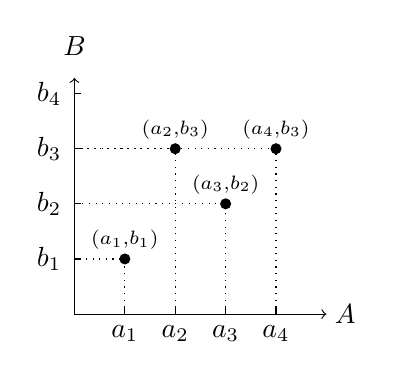
\begin{tikzpicture}[x=0.8cm]
  	\draw[->] (0,0) -- (4,0);
  	\draw[->] (0,0) -- (0,3.0);
  	\node at (4.3,0) {$A$};
  	\node at (0,3.4) {$B$};

      \draw (0.8,0) -- +(0,0.1) node [label=below:$a_1$]{};
      \draw (1.6,0) -- +(0,0.1) node [label=below:$a_2$]{};
      \draw (2.4,0) -- +(0,0.1) node [label=below:$a_3$]{};
      \draw (3.2,0) -- +(0,0.1) node [label=below:$a_4$]{};

      \draw (0,0.7) -- +(0.1,0) node [label=left:$b_1$]{};
      \draw (0,1.4) -- +(0.1,0) node [label=left:$b_2$]{};
      \draw (0,2.1) -- +(0.1,0) node [label=left:$b_3$]{};
      \draw (0,2.8) -- +(0.1,0) node [label=left:$b_4$]{};

  	\draw[dotted] (0.8,0) -- (0.8,0.7) -- (0,0.7);
  	\draw[dotted] (1.6,0) -- (1.6,2.1) -- (0,2.1);
  	\draw[dotted] (2.4,0) -- (2.4,1.4) -- (0,1.4);
  	\draw[dotted] (3.2,0) -- (3.2,2.1) -- (0,2.1);

  	\fill (0.8,0.7) circle (2pt) node[above] {$\scriptstyle (a_1,b_1)$};
  	\fill (1.6,2.1) circle (2pt) node[above] {$\scriptstyle (a_2,b_3)$};
  	\fill (2.4,1.4) circle (2pt) node[above] {$\scriptstyle (a_3,b_2)$};
  	\fill (3.2,2.1) circle (2pt) node[above] {$\scriptstyle (a_4,b_3)$};
  \end{tikzpicture}
\hfill
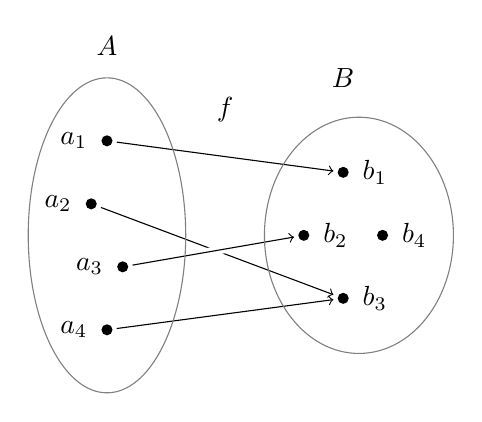
\begin{tikzpicture}[x=1cm,y=0.8cm]
\fill (1,4) circle (2pt) node (a1) [label=left:$a_1$]{};
\fill (0.8,3) circle (2pt) node (a2) [label=left:$a_2$]{};
\fill (1.2,2) circle (2pt) node (a3) [label=left:$a_3$]{};
\fill (1,1) circle (2pt) node (a4) [label=left:$a_4$]{};
\fill (4,3.5) circle (2pt) node (b1) [label=right:$b_1$] {};
\fill (3.5,2.5) circle (2pt) node (b2) [label=right:$b_2$] {};
\fill (4,1.5) circle (2pt) node (b3) [label=right:$b_3$] {};
\fill (4.5,2.5) circle (2pt) node (b4) [label=right:$b_4$] {};
\draw[->] (a1) edge (b1);
\draw[->] (a2) edge (b3);
\draw[line width=3pt,white] (a3) edge (b2);
\draw[->] (a3) edge (b2);
\draw[->] (a4) edge (b3);
\draw[draw=gray](1,2.5) ellipse (1cm and 2cm);
\draw[draw=gray](4.2,2.5) ellipse (1.2cm and 1.5cm);
\node at (1,5.5) {$A$};
\node at (4,5) {$B$};
\node at (2.5,4.5) {$f$};
\end{tikzpicture}
\hfill
\mbox{}
\caption[]{La funzione $f\colon A\to B$,
$f=\{a_1\mapsto b_1,$ $a_2 \mapsto b_3,$ $a_3 \mapsto b_2,$ $a_4 \mapsto b_3\}$
definita sull'insieme $A=\ENCLOSE{a_1, a_2, a_3, a_4}$
a valori nell'insieme $B=\ENCLOSE{b_1, b_2, b_3, b_4}$
rappresentata tramite grafico e
tramite diagrammi di Venn.}
\label{fig:funzione}
\end{figure}

L'insieme di partenza $A$ viene chiamato \emph{dominio}%
\mymargin{dominio}%
\index{dominio} 
della funzione $f\colon A\to B$,
mentre l'insieme di arrivo $B$ viene chiamato \emph{codominio}%
\mymargin{codominio}%
\index{codominio}.
La funzione $f$ rappresenta quindi un modo di assegnare in maniera univoca
ad ogni elemento del dominio un elemento del codominio.
Da un punto di vista informatico potremmo dire che $A$ è l'insieme
dei possibili \emph{input} e $B$ è l'insieme dei possibili \emph{output}
della funzione $f$.

Per come l'abbiamo definita, una funzione è dunque un insieme.
In generale le funzioni potrebbero essere definite in altri modi oppure 
potrebbero essere un concetto primitivo: dunque nei capitoli seguenti useremo le funzioni 
senza assumere che esse siano a loro volta degli insiemi.
Ad esempio invece di scrivere $(a,b)\in f$ scriveremo sempre $f(a)=b$ 
oppure $a\stackrel f \mapsto b$.
Sarà comunque molto importante
considerare l'insieme che rappresenta $f$ ma questo verrà chiamato
\emph{grafico}%
\mymargin{grafico}%
\index{grafico} di $f$, $G_f$ e potrà essere definito in questo modo:
\[
  G_f = \ENCLOSE{(x,y)\in A \times B\colon f(x)=y}.
\]
Nella nostra costruzione risulta effettivamente $G_f = f$ ma, come abbiamo detto,
in generale è opportuno distinguere la funzione dal suo grafico.
Uno degli argomenti principali di questo corso è lo studio 
del grafico delle funzioni reali, cioè le funzioni 
con dominio e codominio nell'insieme dei numeri reali.

\subsection{invertibilità}

Capita molto spesso che un fenomeno possa essere modellizzato matematicamente
tramite una funzione: si sa che ad un certo \emph{input} $a$ corrisponde
un \emph{output} $b=f(a)$. Molto spesso il problema da risolvere è
quello di determinare l'\emph{input} giusto $a$ per ottenere l'\emph{output}
voluto $b$. Questo problema corrisponde ad \emph{invertire} la funzione $f$:
dato $b\in B$ determinare $x\in A$ tale che $f(x) = b$.

Una funzione $f\colon A \to B$ si dice essere \emph{surgettiva}%
\mymargin{surgettiva}%
\index{surgettiva} (o \emph{suriettiva})
se per ogni $b\in B$ esiste almeno un $x\in A$ per cui $f(x)=b$. Questo
significa che il problema dell'inversione ha almeno una soluzione, qualunque
sia $b\in B$.
Una funzione $f\colon A \to B$ si dice essere \emph{iniettiva}%
\mymargin{iniettiva}%
\index{iniettiva}
se non esistono due punti distinti $a,a' \in A$, $a\neq a'$ tali
che $f(a) = f(a')$. Questo significa che il problema dell'inversione
$f(x)=b$ ha al più una soluzione (la soluzione, se esiste, è unica).
Una funzione $f\colon A \to B$ si dice essere \emph{bigettiva}%
\mymargin{bigettiva}%
\index{bigettiva}
(o \emph{biettiva})
\index{biettiva}%
\index{bigettiva}%
\index{funzione!bigettiva}%
\index{invertibile}%
\index{funzione!invertibile}%
\index{biettiva}%
o
\emph{invertibile}%
\mymargin{invertibile}%
\index{invertibile}%
\mynote{\textbf{Attenzione:} in alcuni testi (tra cui~\cite{Giusti}) si considerano
invertibili le funzioni iniettive, anche se non surgettive.}
se è sia iniettiva che surgettiva. Questo significa
che il problema dell'inversione $f(x)=b$ ha una unica soluzione $x\in A$
qualunque sia $b\in B$. In particolare, se $f$ è invertibile, per ogni $b\in B$ esiste
un unico $a\in A$ per cui $f(a)=b$.
Se $f$ è una funzione invertibile allora la relazione inversa $g$
cioè la relazione tale che $b\stackrel g \mapsto a$ quando $a \stackrel f \mapsto b$
risulta essere una funzione $g\colon B\to A$. 
Infatti $g$ è definita su tutto $B$ in quanto $f$ è surgettiva 
e $g$ è univoca in quanto $f$ è iniettiva.
Le proprietà caratteristiche della \emph{funzione inversa}%
\mymargin{funzione inversa}%
\index{funzione!inversa} $g$ sono:
\begin{equation}\label{eq:572098}
  \forall a\in A\colon g(f(a)) = a, \qquad
  \forall b\in B\colon f(g(b)) = b.
\end{equation}
La funzione $g$ inversa di $f$ viene usualmente denotata con il simbolo $f^{-1}$.

Se $f\colon A\to B$ è bigettiva diremo che $A$ 
e $B$ sono in \emph{corrispondenza biunivoca}%
\mymargin{corrispondenza biunivoca}%
\index{corrispondenza!biunivoca} tramite $f$.
In effetti $f$ è una corrispondenza \emph{univoca} da $A$ in $B$
(manda in modo univoco ogni punto di $A$ in un punto di $B$)
e $f^{-1}$ è una corrispondenza univoca da $B$ in $A$.

Introduciamo ora delle notazioni che sarà comodo utilizzare nel seguito.
Se $f\colon A \to B$ è una funzione e se $C\subset A$ definiamo
\[
  f(C) 
  = \ENCLOSE{f(a)\colon a \in C} 
  = \ENCLOSE{b\in B\colon \exists a\in C\colon b=f(a)}.
\]
L'insieme $f(C)\subset B$ si chiama \emph{immagine}%
\mymargin{insieme immagine}%
\index{immagine}
\index{immagine!insieme}%
di $C$ (tramite $f$) ed è formato
da tutti i punti che si ottengono applicando $f$ agli elementi di $C$.
L'immagine $f(A)$ dell'intero dominio $A$ si chiama immagine di $f$
e si denota a volte con il simbolo $\Im f$.
Si noti che $f$ è surgettiva se e solo se $f(A)=B$ (cioè se l'immagine coincide
col codominio).
Ad esempio la funzione definita in Figura~\ref{fig:funzione}
ha immagine $f(A) = \ENCLOSE{f(a_1),f(a_2),f(a_3),f(a_4)} 
 = \ENCLOSE{b_1, b_2, b_3}$.

Anche se $f\colon A \to B$ non fosse iniettiva,
per ogni $C\subset B$ possiamo definire
\[
  f^{-1}(C) = \ENCLOSE{a\in A\colon f(a) \in C}.
\]
L'insieme $f^{-1}(C)\subset A$ si chiama \emph{preimmagine}
o \emph{controimmagine}
\mymargin{preimmagine}%
\index{preimmagine}%
\index{preimmagine!insieme}%
\index{controimmagine!insieme}%
\index{insieme!controimmagine}%
di $C$ (tramite $f$)
ed è formato da tutti i punti di $A$ che applicando $f$ vanno in $C$.
Si noti che se $b\in B$ l'insieme $f^{-1}(\ENCLOSE{b})$ non è altro che
l'insieme delle soluzioni dell'equazione $f(x)=b$. Come abbiamo
già visto tale insieme contiene almeno un elemento se $f$ è suriettiva,
contiene al più un elemento se $f$ è iniettiva e contiene esattamente
un elemento $f^{-1}(\ENCLOSE{b}) = \ENCLOSE{f^{-1}(b)}$ se $f$ è bigettiva.
Ad esempio se $f$ è la funzione definita in figura~\ref{fig:funzione}
si ha $f^{-1}(\ENCLOSE{b_3,b_4}) = f^{-1}(\ENCLOSE{b_3}) = \ENCLOSE{a_2,a_4}$,
$f^{-1}(\ENCLOSE{b_4}) = \emptyset$.


La notazione $f(C)$ appena introdotta è formalmente ambigua in quanto
potrebbe non essere chiaro se $C$ è un elemento oppure un sottoinsieme
del dominio di $f$.
In pratica il contesto dovrebbe rendere chiaro cosa si intende.

Più in generale ci capiterà di estendere questo abuso di notazione non solo
alle funzioni, ma anche alle relazioni e alle operazioni.
Ad esempio se $A$ e $B$ sono insiemi di numeri ci capiterà di scrivere $A\le B$
per intendere che ogni elemento di $A$ è minore o uguale ad ogni elemento di $B$
oppure $A+B$ per intendere l'insieme di tutti i numeri che si ottengono sommando
ogni numero elemento di $A$ ad ogni numero elemento di $B$.

\begin{exercise}
  Sia $f\colon A \to B$ una funzione qualunque. 
  Si verifichi che se $C\subset A$ e $D\subset B$ si ha 
  \[
    f^{-1}(f(C))\supset C,
    \qquad 
    f(f^{-1}(D)) \subset D. 
  \]
  
  Che ipotesi possiamo fare su $f$ per avere l'uguaglianza
  $f(f^{-1}(C)) = C$?
  E per avere $f^{-1}(f(D)) = D$?
\end{exercise}

Si osservi che se $f\colon A \to B$ è una funzione e 
se $C\supset f(A)$ allora risulta anche $f\colon A \to C$ in quanto 
i valori di $f$ sono elementi di $C$. 
Dunque il \emph{codominio} di una 
funzione può essere esteso o ristretto con l'accortezza di mantenere 
tutti i valori dell'immagine. 
In particolare $f\colon A \to f(A)$ è certamente surgettiva.

Ad esempio vedremo che la funzione $\sin$ 
sarà definita con dominio l'insieme $\RR$ dei numeri reali 
ma può avere come codominio sia $\RR$ stesso
che solamente l'intervallo $[-1,1]$ dei numeri compresi 
tra $-1$ e $1$. 
Non ha quindi senso chiedersi se $\sin$ è suriettiva finché 
non dichiaro qual è il codominio considerato:
$\sin\colon \RR\to[-1,1]$ è suriettiva mentre 
$\sin\colon \RR\to\RR$ non lo è. 
Altri testi considerano il codominio parte della definizione 
della funzione e quindi considerano diverse due funzioni 
che hanno lo stesso grafico ma codominio diverso. 
E' una sottigliezza di poca rilevanza.

Per rendere iniettiva una funzione dobbiamo invece restringere il dominio.

\begin{definition}[restrizione]
  \label{def:restrizione}%
  Se $f\colon A\to B$ è una funzione e $C\subset A$, possiamo 
  \emph{restringere} il dominio di $f$ all'insieme $C$.
  \mynote{La notazione $f\llcorner C$ non è del tutto standard,
  probabilmente è più comune la notazione $f_{|C}$.}%
  Si ottiene una nuova funzione $f\llcorner C$ che coincide con $f$
  ma che è definita solo su $C$: $f\llcorner C\colon C\to B$:
  \[
  f\llcorner C(x) = f(x)\qquad 
  \forall x \in C.
  \]
\end{definition}


\subsection{funzione composta}
\index{composizione!di funzioni}%

Se $f\colon A\to B$ e $g\colon B\to C$ allora un punto $a\in A$ 
viene mandato tramite $f$ in un punto $b\in B$ e 
a sua volta il punto $b$ viene mandato da $g$ in un punto 
$c \in C$. 
La funzione che manda $a$ in $c$ viene chiamata 
\emph{funzione composta}%
\mymargin{funzione composta}%
\index{funzione!composta} si denota con $g\circ f$ 
e si può definire così:
\[
g\circ f \colon A \to C, \qquad 
(g\circ f)(x) = g(f(x)).  
\]

Se abbiamo tre funzioni 
$f\colon A\to B$, $g\colon B\to C$ e $h\colon C\to D$ 
allora è facile verificare che:
\[
   h \circ (g\circ f) = (h\circ g) \circ f
\]
in quanto per ogni $x\in A$ si ha
\[
(h \circ (g\circ f)) (x) =
h(g(f(x))) = (h\circ g)(f(x)) = ((h\circ g) \circ f) (x).  
\]
Significa che l'operatore di composizione $\circ$
soddisfa la proprietà associativa.

Se $f\colon A\to B$ è bigettiva allora 
per ogni $x\in A$ e per ogni $y\in B$ si ha,
grazie a~\eqref{eq:572098},
\[
  f^{-1} (f(x)) = x,
  \qquad f(f^{-1}(y)) = y.
\]
Significa che 
\[
  f^{-1}\circ f = \id_A, 
  \qquad
  f\circ f^{-1} = \id_B
\] 
dove $\id_X\colon X\to X$
è la funzione 
\emph{identità}%
\mymargin{identità}%
\index{identità} 
\index{funzione!identità}%
cioè la funzione 
che lascia fisso ogni punto di $X$:
\mymargin{$\id_X$}%
\index{$\id$}%
\[
\id_X(x) = x \qquad \text{per ogni $x\in X$}.
\]

\begin{theorem}
Se $f\colon A\to B$ e $g\colon B\to C$ sono entrambe invertibili
anche $g\circ f\colon A\to C$ è invertibile e si ha 
\begin{equation}\label{eq:inversa_composta}
  (g\circ f)^{-1} = f^{-1}\circ g^{-1}.
\end{equation}
\end{theorem}
\begin{proof}    
Per ogni $c\in C$ esiste un unico $b\in B$ tale che $g(b)=c$ 
ed un unico $a\in A$ tale che $f(a)=b$. 
Tale $a$ è l'unico punto per cui $g(f(a))=c$ e questo dimostra che 
$g\circ f$ è bigettiva. Inoltre $a=f^{-1}(b)$ e $b=g^{-1}(c)$ 
dunque $(g\circ f)^{-1}(c) = a = f^{-1}(g^{-1}(c))$ da cui si ottiene 
\eqref{eq:inversa_composta}.
\end{proof}

\begin{exercise}
  Si verifichi che la composizione di funzioni iniettive è iniettiva e la composizione 
  di funzione suriettive è suriettiva.
\end{exercise}

\section{strutture algebriche}

Andremo presto a definire strutture numeriche su cui sono definite le operazioni 
di addizione e moltiplicazione. 
In generale vogliamo definire cosa si intende con una \emph{operazione}.
\mymargin{operazione}%
\index{operazione}%

Una \emph{operazione} sull'insieme $A$ è una funzione 
$f\colon A\to(A\to A)$.
Dati $a,b\in A$ avremo dunque che $f(a)$ è una funzione $A\to A$
e quindi $f(a)(b)$ sarà un elemento di $A$. 
Tipicamente le operazioni si denotano con simboli come $+$, $\cdot$, $\div$, $\times$ etc...
Se $*$ è una operazione, invece di scrivere $*(a)(b)$ scriveremo 
$a*b$.

Si noti che una funzione $f\colon A\to (A\to A)$ è equivalente ad una funzione
$g\colon A\times A \to A$ ponendo $g(a,b) = f(a)(b)$. 
Si può dunque pensare equivalentemente ad una operazione 
come ad una funzione di due variabili.

\begin{example}
La usuale operazione di addizione $+$ definita sugli insiemi numerici è una operazione.
Se $\NN$ è l'insieme dei numeri naturali (lo definiremo tra poco)
possiamo pensare a $+\colon \NN\to (\NN\to \NN)$ come ad una funzione che ad un 
numero $n\in \NN$ associa la funzione $+n$ che incrementa di $n$ il suo argomento:
$(+3)(5)=3+5=8$.
\end{example}

Quando i simboli delle operazioni vengono utilizzati in una espressione si pone 
il problema di stabilire la precedenza delle operazioni.
Se ad esempio scriviamo $a*b*c$ dobbiamo decidere se intendiamo
$(a*b)*c$ (associatività a sinistra) oppure $a*(b*c)$ (associatività a destra).
Se $(a*b)*c=a*(b*c)$ diremo che l'operazione è associativa, in tal 
caso ovviamente non importa specificare se è associativa a sinistra o a destra.
Usualmente si intende che l'operazione è associativa a sinistra.
Ad esempio $5-4-3 = (5-4)-3$ e non $5-(4-3)$. 
In alcuni rari casi l'associatività è a destra, un esempio tipico è l'elevamento 
a potenza: $2^{3^2} = 2^{(3^2)} \neq (2^3)^2$.
Il motivo è che $(a^b)^c$ si scrive più facilmente $a^{b\cdot c}$.
Nei linguaggi di programmazione che implementano l'operazione di elevamento 
a potenza bisogna fare molta attenzione: in alcuni linguaggi (ad esempio Fortran) 
l'elevamento a potenza 
associa a sinistra come le altre operazioni, in altri linguaggi (ad esempio Python)
associa a destra.

Quando compaiono operazioni diverse nella stessa espressione, alcune operazioni 
hanno la precedenza su altre.
Ad esempio in $a+b\cdot c$ la moltiplicazione ha la precedenza sull'addizione
e quindi l'espressione va interpretata come $a+(b\cdot c)$ non come $(a+b)\cdot c$.
Addizione e sottrazione hanno la stessa precedenza e vanno quindi interpretate da sinistra a destra:
$a-b+c = (a-b)+c$. Per la divisione noi useremo, raramente, il simbolo $/$, 
in tal caso la divisione associa a sinistra ed ha la stessa precedenza della 
moltiplicazione: $a/b/c=(a/b)/c$, $a/b\cdot c=(a/b)\cdot c$.
Questa regola è a volte controintuitiva, per cui noi eviteremo di scrivere 
espressioni di questo tipo, soprattutto perché il puntino della moltiplicazione 
può essere omesso, come in $a/bc$ rendendo l'espressione ancora più ambigua.
Nel dubbio: usare le parentesi!
Per denotare la divisione utilizzeremo più spesso il simbolo di frazione $\frac a b$ che non richiede 
di specificare l'associatività e la precedenza in quanto la lunghezza della 
linea di frazione determina come vengono associati gli operandi: 
\[
  \frac{\,\frac a b\,}{c}=(a/b)/c, \qquad 
  \frac{a}{\,\frac bc\,}=a/(b/c).
\]  

Gli insiemi numerici che ci proponiamo di definire (naturali, interi, razionali, reali, complessi)
sono dotati tutti delle due operazioni di addizione e moltiplicazione
oltre che (salvo i numeri complessi) di una relazione di ordine.
In base alle proprietà che queste operazioni soddisfano potranno rientrare nelle 
seguenti strutture algebriche astratte. 

Per adesso facciamo un elenco delle strutture che incontreremo più avanti. 
Man mano che individueremo gli esempi di insiemi che rientrano in queste strutture
sarà più chiaro il significato di queste definizioni.

\begin{definition}[monoide]%
  \label{def:monoide}%
  Sia $A$ un insieme su cui è definita una operazione $*$.
  Se l'operazione è associativa: $x*(y*z) = (x*y)*z$ 
  ed ha elemento neutro $e\in A$ tale che $e*x = x*e = x$
  diremo che $A$ è un \emph{monoide}.
  Se inoltre l'operazione è commutativa, $x*y=y*x$ 
  diremo che $A$ è un \emph{monoide commutativo} (o abeliano).
  
  Quando per l'operazione $*$ viene utilizzato il simbolo di addizione $+$
  diremo che il monoide è additivo. In tal caso l'elemento neutro 
  si chiama \emph{zero} e si indica con $0$.
  Se utilizziamo invece il simbolo di moltiplicazione $x\cdot y$
  diremo che il monoide è moltiplicativo. In tal caso l'elemento 
  neutro si chiama \emph{unità} e si indica usualmente con $1$.
  \end{definition}
  
  \begin{example}
  L'insieme dei numeri naturali è un monoide commutativo sia con l'operazione di addizione $+$ 
  (monoide additivo) che con l'operazione di moltiplicazione 
  $\cdot$ (monoide moltiplicativo).
  \end{example}
  
  \begin{definition}[gruppo]
  \label{def:gruppo}%
  Un insieme $G$ su cui è definita una \emph{operazione} $*$ 
  si dice essere un \emph{gruppo}%
\mymargin{gruppo}%
\index{gruppo} se l'operazione
  ha le seguenti proprietà:
  \begin{enumerate}
    \item associativa: $\forall x,y,z\in G\colon (x*y)*z = x*(y*z)$;
    \index{proprietà!associativa}%
    \index{associatività}%
    \item esistenza elemento neutro: 
    \index{elemento!neutro}%
    \index{neutro}%
    $\exists e\in G\colon \forall x\in G \colon e*x=x*e = x$;
    \item esistenza inverso: 
    \index{elemento!inverso}%
    \index{inverso}%
    $\forall x\in G\colon \exists y\in G\colon x*y=y*x=e$.
  \end{enumerate}
  Inoltre il gruppo si dice essere \emph{abeliano}%
\mymargin{gruppo abeliano}%
\index{abeliano} o \emph{commutativo}
  se vale la proprietà:
  \begin{enumerate}
    \item[4.] commutativa: $\forall x,y\in G\colon x*y = y*x$.
    \index{proprietà!commutativa}%
    \index{commutatività}% 
  \end{enumerate}
  
  Quando l'operazione viene denotata con il simbolo $+$ (addizione)
  diremo che il gruppo è additivo, denoteremo con $0$ 
  \index{zero}%
  (zero) l'elemento neutro e l'inverso di $x$ verrà chiamato \emph{opposto}
  e si denota con $-x$.
  \index{opposto}%
  Se invece si usa il simbolo $\cdot$ (moltiplicazione)
  diremo che il gruppo è moltiplicativo, l'elemento neutro potrà 
  essere denotato con il simbolo $1$ (uno o unità) e 
  \index{uno}\index{unità}%
  l'inverso di $x$ potrà essere chiamato \emph{reciproco}
  e si denota usualmente con $x^{-1}$ o $\frac 1 x$.
  \index{reciproco}%
\end{definition}
  
L'elemento neutro di un gruppo è unico. 
Se infatti $x$ e $y$ fossero due elementi neutri 
si avrebbe $x = x*y = y$. 
Anche l'inverso è unico: infatti se $y$ e $z$ fossero 
due inversi di $x$ si avrebbe $y = y * x * z = z$.

\begin{example}
  L'insieme dei numeri interi $\ZZ$ con l'operazione di addizione 
  è un gruppo abeliano. 
  L'elemento neutro è lo zero, l'opposto di $x$ è $-x$.
  Su $\ZZ$ definiremo anche l'operazione di moltiplicazione,
  ma $\ZZ$ con l'operazione di moltiplicazione non è un gruppo 
  in quanto non tutti gli elementi hanno inverso moltiplicativo in $\ZZ$.
\end{example}

\begin{example}[gruppo simmetrico]
  Se $X$ è un insieme qualunque si può considerare l'insieme
  $X!$ delle funzioni bigettive su $X$:
  \[
    X! = \ENCLOSE{f\colon X\to X\colon f \text{ bigettiva}}.
  \]
  Quando $X$ è un insieme finito le funzioni bigettive su $X$ si chiamano 
  anche \emph{permutazioni} in quanto, appunto, permutano gli elementi di $X$.

  Per esercizio si può verificare che l'operazione $\circ$ di composizione 
  rende $X!$ un gruppo.
  Tale gruppo si chiama \emph{gruppo simmetrico} di $X$ 
  (viene anche usualmente denotato con $S_X$).
  Il gruppo simmetrico non è abeliano se $X$ ha più di due elementi.
\end{example}

\begin{definition}[anello e campo]
  \label{def:anello}%
  \label{def:campo}%
  Sia $A$ un insieme su cui sono definite due operazioni: 
  addizione e moltiplicazione.  
  Diremo che $A$ è un \emph{anello} se $A$ è un gruppo abeliano rispetto alla 
  addizione, 
  se la moltiplicazione è associativa $(x\cdot y)\cdot z = x\cdot (y\cdot z)$ 
  e se vale la proprietà distributiva $x\cdot(y+z) = x\cdot y + x\cdot z$,
  $(x+y)\cdot z = x\cdot z + y\cdot z$.

  Se inoltre esiste un elemento $1\in A$ neutro per la moltiplicazione 
  diremo che $A$ è un anello \emph{con unità}.

  Se la moltiplicazione è commutativa diremo che $A$ è un \emph{anello abeliano}.

  Se $A$ è un anello ed $A\setminus \ENCLOSE{0}$ risulta essere un gruppo abeliano
  per l'operazione di moltiplicazione 
  (dunque c'è una unità $1\neq 0$ e ogni elemento non nullo ha inverso moltiplicativo)
  diremo che $A$ è un \emph{campo}.
\end{definition}

\begin{example}
  L'insieme dei numeri interi $\ZZ$ (lo definiremo tra poco) è un anello abeliano con unità
  ma non è un campo.
  L'insieme dei numeri razionali $\QQ$ (lo definiremo tra poco) è un campo.
\end{example}

Un anello $A$ è un gruppo additivo, per cui negli anelli l'elemento neutro 
dell'addizione si indica con $0$. 
L'inverso additivo di $a\in A$ si chiama \emph{opposto} e si indica con $-a$.
E' quindi definita anche l'operazione di sottrazione: $a-b = a+(-b)$.

Lo stesso vale in un campo $R$ dove, inoltre, ogni elemento non nullo ha 
anche un inverso moltiplicativo. Se $x\in R\setminus\ENCLOSE{0}$ il suo
inverso moltiplicativo si chiama \emph{reciproco} e si indica con $1/x$ oppure $x^{-1}$.
Dunque è definita anche l'operazione di divisione: $a/b = a\cdot (1/b)$
se $b\neq 0$.

In generale se $A$ è un anello allora valgono
le familiari proprietà:
\[
  0\cdot x = x\cdot 0 = 0, \qquad
  (-1)\cdot x = x \cdot (-1) = -x.
\]
Per la prima abbiamo: 
\[
  0\cdot x = 0\cdot x + x + (-x) = (0+1)\cdot x + (-x) = x + (-x) = 0
\]
e scrivendo gli addendi in ordine opposto si ottiene anche $x\cdot 0 = 0$.
Diremo che $0$ è \emph{elemento assorbente}
\mymargin{elemento assorbente}%
\index{elemento!assorbente}%  
\index{assorbente}%
per la moltiplicazione.
Allora possiamo dimostrare anche la seconda proprietà:
\[
   (-1)\cdot x = (-1)\cdot x + x + (-x) = (-1 + 1)\cdot x + (-x) = 0 + (-x) = -x
\]
e anche in questo caso scrivendo gli addendi in ordine opposto si ottiene $x\cdot(-1)=-x$.

Se $A$ è un campo, vale la legge di \emph{annullamento del prodotto}:
\index{annullamento!prodotto}%
\mymargin{annullamento prodotto}%
\[
  x\cdot y = 0 \iff x=0 \lor y=0.
\]
L'implicazione verso sinistra è la proprietà assorbente, che abbiamo già 
verificato. 
Viceversa se $x\cdot y = 0$ e $x\neq 0$ allora possiamo moltiplicare
ambo i membri per $x^{-1}$ e ottenere $y=x^{-1}\cdot 0 = 0$.

\begin{definition}[gruppo totalmente ordinato]
  \label{def:gruppo_ordinato}%
  \label{def:campo_ordinato}%
  Diremo che $G$ è un \emph{gruppo totalmente ordinato}
\mymargin{gruppo totalmente ordinato}%
\index{gruppo!ordinato}% 
  se $G$ è un gruppo
  (con operazione $*$),
  se è anche un insieme totalmente ordinato (con relazione $\le$)
  e se l'operazione del gruppo mantiene 
  l'ordinamento ovvero vale la proprietà
  \begin{enumerate}
    \item[1.] monotonia:
    se $x\le y$ allora per ogni $z$ si ha:
      \[
      x*z \le y*z \qquad\text{e}\qquad z*x \le z*y.
      \] 
  \end{enumerate}
  Diremo che il gruppo totalmente ordinato, 
  è \emph{denso} o \emph{continuo} se la relazione 
  d'ordine ha anche tali proprietà.

  Diremo che $R$ è un \emph{campo ordinato}
\mymargin{campo ordinato}%
\index{campo!ordinato}%
  se è un campo, 
  se rispetto alla addizione 
  è un gruppo abeliano totalmente ordinato
  (dunque l'addizione preserva l'ordinamento 
  $x\le y \implies x+z\le y+z$)
  e se inoltre anche la moltiplicazione per un numero positivo 
  mantiene l'ordinamento:
  \begin{enumerate}
    \item[2.] monotonia: 
    se $x\le y$ e $0\le z$ allora $x\cdot z \le y\cdot z$. 
  \end{enumerate} 

  Diremo che il campo ordinato è \emph{continuo} 
  se l'ordinamento è continuo.
\end{definition}

\begin{example}
Vedremo che $\ZZ$ (l'insieme dei numeri interi) è un esempio di gruppo additivo totalmente ordinato 
ma non denso.
\end{example}

\begin{example}
Vedremo che $\QQ$ (i numeri razionali) è un esempio di campo ordinato denso ma non continuo 
mentre $\RR$ (i numeri reali) è un (in un certo senso l'unico) esempio di campo ordinato continuo.
\end{example}

\begin{example}
Un esempio banale di gruppo totalmente ordinato denso e continuo è $X=\ENCLOSE{0}$.
\end{example}

Se $G$ è un gruppo additivo totalmente ordinato con elemento neutro $0$ si ha:
\[
  x\le y  \iff 0 \le y-x.
\]
Significa che l'ordinamento è univocamente determinato 
dal confronto con l'elemento neutro, ovvero dal sapere 
quali sono gli elementi positivi.

Se $G$ è un gruppo additivo totalmente ordinato, possiamo esprimere una proprietà di monotonia 
per le disuguaglianze strette: se $x<y$ allora $x+z<y+z$ e $z+x<z+y$.
Si tratta di osservare che se vale l'uguaglianza $x+z=y+z$,
sommando $-z$ ad ambo i membri si ottiene $x=y$.

Se $R$ è un campo ordinato e prendiamo $x\in R$, 
Possiamo osservare che $x\ge 0$ se e solo se $-x\le 0$. 
Infatti basta sommare alla prima disequazione $-x$
per ottenere la seconda e viceversa sommare $x$ alla seconda per 
ottenere la prima (monotonia dell'addizione).

Verifichiamo ora la validità della regola dei segni per il prodotto:
se $x\ge 0$ e $y\ge 0$ allora $x\cdot y \ge 0$,
$(-x)\cdot (-y) \ge 0$, $(-x)\cdot y = x \cdot (-y) \le 0$.
La prima proprietà, $x\cdot y\ge 0$ è data per ipotesi (proprietà di monotonia 
del prodotto applicata a $y\ge 0$ moltiplicando ambo i membri per $x\ge 0$).
Di conseguenza $-(x\cdot y)\le 0$, ovvero $(-x)\cdot y \le 0$ 
e $x\cdot (-y) \le 0$. 
Cambiando ancora segno a quest'ultima disuguaglianza si ottiene $(-x)\cdot(-y)\ge 0$.

Dunque possiamo dedurre che per ogni $x\in R$ si ha $x^2=x\cdot x\ge 0$
perché sia che $x\ge 0$ sia che $x\le 0$ il prodotto sarà sempre $\ge 0$.

In particolare possiamo dedurre che $1=1\cdot 1\ge 0$. 
E visto che per ipotesi di campo, $1\neq 0$ si deve avere $1>0$.

\begin{exercise}
Sia $R$ un campo ordinato, $m\in R$, $m>0$.
Allora $m^{-1}>0$.
Inoltre (se $m>0$) per ogni $x,y\in R$ si ha:
\[
  x<y \iff m\cdot x < m\cdot y.
\]
\end{exercise}

\begin{exercise}
Dimostrare che ogni campo ordinato è denso.
\end{exercise}
\begin{proof}[Svolgimento.]
Dati $x,y\in R$ con $x<y$ dobbiamo trovare $z\in R$ tale che $x<z<y$.
Se $x<y$ si ha, $x+x<y+x<y+y$, 
\end{proof}


\section{i numeri naturali}
\label{sec:naturali}

Sebbene le proprietà dei numeri naturali dovrebbero essere intuitivamente già ben note,
la loro formalizzazione non è banale.
In particolare alcune dimostrazioni risultano complicate perché quando dobbiamo dimostrare 
molti fatti ovvi, bisogna fare attenzione a non utilizzare proprietà che ci risultano ovvie 
ma che ancora non sono state dimostrate.
Per questo motivo è perfettamente legittimo se in prima lettura saltiamo le dimostrazioni 
per capire il senso generale del discorso e poi, se necessario, torniamo indietro per
approfondire i dettagli.

I numeri naturali $0,1,2,\dots$ sono i numeri che utilizziamo per contare o per 
fare le iterazioni. C'è un primo numero naturale, che per noi sarà $0$, e poi
per ogni numero naturale $n$ ce n'è uno successivo che chiameremo $\sigma(n)$. 
Partendo da $0$ e passando al successivo si raggiungono tutti i numeri naturali.

\begin{definition}[assiomi di Peano]
  \label{def:assiomi_peano}%
  \label{def:naturali}%
  \mynote{Giuseppe Peano (1858--1932) vedi note storiche a pag.~\pageref{nota:Peano}} 
  \index{numeri!naturali}%
  \index{$\NN$}%
  \index{Peano}%
  \index{assiomi!di Peano}%
  \index{insieme!induttivo}%
  \index{induttivo}%
Dato un insieme $\NN$, 
un elemento $0\in \NN$ 
e una funzione $\sigma\colon \NN\to\NN$ 
diremo che $(\NN,0,\sigma)$
soddisfa gli assiomi di Peano,
o più semplicemente che $\NN$ è un insieme di numeri naturali,
se valgono le seguenti proprietà: 
\mynote{La funzione $\sigma$ ci dà il successore di ogni numero. 
Definiremo $1=\sigma(0)$, $2=\sigma(2)$, $3=\sigma(2)$, \dots
Il primo assioma di Peano dice che numeri diversi hanno 
numeri successori diversi. 
Il secondo assioma ci dice che il primo 
numero naturale, per noi lo $0$, 
non è il successore di nessun'altro mentre ogni altro numero 
ne ha uno precedente. Il terzo assioma, il principio di induzione, 
ci dice che ogni numero naturale può essere raggiunto dallo $0$ 
facendo un numero finito di passaggi al successore.}
\begin{enumerate}
  \item $\sigma$ è iniettiva;
  \item $\sigma(\NN) = \NN \setminus\ENCLOSE{0}$;
  \item se $A\subset \NN$ e 
  \begin{enumerate} 
    \item[(i)] $0\in A$ 
    \item[(ii)] $n\in A \implies \sigma(n)\in A$
  \end{enumerate}
  allora $A=\NN$.
\end{enumerate}
\end{definition}

Nel seguito supporremo sempre che $\NN$ sia un insieme che soddisfa la precedente definizione.
Vedremo nel Teorema~\ref{th:unicitaN} che due diversi insiemi che soddisfano gli assiomi di Peano 
sono isomorfi, cioè possono essere messi in corrispondenza biunivoca mantenendo la stessa struttura.
In questo senso possiamo dire che gli assiomi di Peano caratterizzano univocamente 
l'insieme dei numeri naturali. 
Diremo quindi che $\NN$ è \emph{l}'insieme dei numeri naturali piuttosto 
che \emph{un} insieme di numeri naturali.

Dato $n\in \NN$ il numero $\sigma(n)$ si chiama il \emph{successore}%
\mymargin{successore}%
\index{successore} di $n$. 
Il numero $0\in \NN$, che per assioma non è il successore di nessun'altro 
numero naturale, si chiama \emph{zero}%
\mymargin{zero}%
\index{zero}. 
Per comodità diamo un nome amche alle altre \emph{cifre decimali}%
\mymargin{cifre decimali}%
\index{cifre!decimali}%
ovvero ai primi numeri naturali
(più avanti introdurremo la notazione posizionale per poter rappresentare ogni numero naturale 
con una sequenza di cifre decimali):
\begin{equation}\label{eq:cifre}
\begin{gathered}
 1 \defeq \sigma(0),\quad  
 2 \defeq \sigma(1),\quad
 3 \defeq \sigma(2),\quad 
 4 \defeq \sigma(3),\quad
 5 \defeq \sigma(4),\\ 
 6 \defeq \sigma(5),\quad 
 7 \defeq \sigma(6),\quad 
 8 \defeq \sigma(7),\quad 
 9 \defeq \sigma(8)
\end{gathered}
\end{equation}
e osserviamo che $\sigma$ è l'usuale operazione del contare:
 \[
 0 \stackrel\sigma\mapsto 1 \stackrel\sigma\mapsto 2 \stackrel\sigma\mapsto 
 3 \stackrel\sigma\mapsto 4 \stackrel\sigma\mapsto 5 \stackrel\sigma\mapsto 
 6 \stackrel\sigma\mapsto \dots  n \stackrel\sigma\mapsto \sigma(n) \dots
 \]

I primi due assiomi di Peano (definizione~\ref{def:assiomi_peano}) 
servono a garantire che in questo processo del \emph{contare}%
\mymargin{contare}%
\index{contare}
troviamo sempre numeri diversi (non si torna mai indietro) in quanto nessun numero 
può avere come successore $0$ o un numero già incontrato in precedenza (che 
se non è zero è il successore di un altro numero).
Questa proprietà è per certi versi paradossale
(paradosso di Galileo, o paradosso dell'hotel Hilbert)
\index{paradosso!di Galileo}%
\index{paradosso!degli insiemi infiniti}%
\index{hotel Hilbert}%
\index{Hilbert!hotel}%
ed per Dedekind è la definizione di insieme infinito (tra poco la andremo a introdurre).%
\mynote{Galileo Galilei (1564--1642) vedi note storiche a pag.~\pageref{nota:Galileo}}%

Gli assiomi che abbiamo visto finora non garantiscono l'esistenza di insiemi infiniti, e dunque se 
vogliamo garantire che l'insieme dei numeri naturali effettivamente esiste, 
dobbiamo aggiungere un ulteriore assioma. 

Potremmo semplicemente richiedere per assioma che esiste un insieme $\NN$ che soddisfa gli assiomi
di Peano~\ref{def:assiomi_peano}.
Ad esempio potremmo richiedere 
che esista l'insieme degli ordinali di Von Neumann \eqref{eq:vonNeumann}. 
\mynote{
Se denotiamo con $P(\alpha)$ il predicato 
$(\emptyset\in \alpha \land \forall n\colon n\in \alpha) \implies n\cup\ENCLOSE{n}\in \alpha$
allora l'assioma che garantisce l'esistenza dell'insieme $\omega$ degli ordinali finiti 
può essere scritto nella forma:
  $\exists \omega\colon (P(\omega) \land \forall \alpha\colon P(\alpha)\implies \omega\subset \alpha)$.
  La funzione $\sigma\omega\colon\omega$ sarebbe quindi $\sigma(n) = n\cup\ENCLOSE n$.
}

Ma sembra più naturale richiedere più semplicemente che esista almeno un insieme infinito,
vedremo infatti che questo è sufficiente a garantire l'esistenza dell'insieme dei numeri naturali
(teorema~\ref{th:esistenza_naturali}, dove si dimostra che ogni insieme infinito contiene un insieme 
che soddisfa gli assiomi di Peano).

Investighiamo quindi per un attimo cosa significa che un insieme sia infinito.
Per dare una definizione indipendente dall'esistenza dei numeri naturali possiamo usare 
una idea dovuta a Dedekind:
un insieme $X$ è infinito se può essere messo in corrispondenza 
biunivoca con un suo sottoinsieme proprio: 
esiste $f\colon X\to X$ tale che $f$ è iniettiva ma non suriettiva. 
Intuitivamente questo non può succedere su un insieme finito: 
se $X$ è finito ci aspettiamo che ogni suo sottoinsieme sia strettamente più piccolo di $X$
e quindi non possa essere messo in corrispondenza con tutto $X$.

\begin{definition}[insieme infinito]
  \label{def:infinito}%
  Diremo che un insieme $X$ è \emph{finito}
  \index{insieme!finito}%
  \index{finito!insieme}%
  \index{Dedekind!finito}%
  (più precisamente: Dedekind-finito)
  se ogni funzione iniettiva $f\colon X\to X$ è anche suriettiva.
  \mymargin{insieme finito}%
\index{insieme finito}%

  Diremo che un insieme $X$ è \emph{infinito} 
  (più precisamente Dedekind-infinito)
  \index{insieme!infinito}%
  \index{infinito!insieme}%
  \index{Dedekind!infinito}%
  se non è finito ovvero
  se esiste $f\colon X\to X$ iniettiva ma non suriettiva.
  \mymargin{insieme infinito}%
\index{insieme infinito}%
\end{definition}

Come abbiamo già osservato gli assiomi di Peano (definizione~\ref{def:assiomi_peano}) 
richiedono che la funzione $\sigma\colon \NN\to\NN$ sia iniettiva ma non suriettiva.
Risulta quindi che $\NN$ deve essere un insieme infinito.

Ma non si può escludere che tutti gli insiemi siano finiti (e che quindi $\NN$ non esista) 
se non introduciamo il seguente assioma.

\begin{axiom}[infinito]
  \label{axiom:infinito}%
  Esiste un insieme infinito. 
\end{axiom}

Grazie al precedente assioma il teorema seguente garantisce
l'esistenza di un insieme $\NN$ che soddisfa gli assiomi di Peano.

\begin{theorem}[esistenza dei numeri naturali]
  \label{th:esistenza_naturali}%
Se $X$ è un qualunque insieme infinito (definizione~\ref{def:infinito})
esistono $\NN\subset X$, $0\in \NN$ e $\sigma\colon \NN\to\NN$ 
che soddisfano gli assiomi di Peano (definizione~\ref{def:assiomi_peano}).
\end{theorem}
%
\begin{proof}
Se $X$ è infinito esiste $f\colon X\to X$ iniettiva ma non suriettiva. 
Scegliamo arbitrariamente $0\in X\setminus f(X)$. 
Preso un sottoinsieme $I\subset X$ diremo che $I$ è \emph{induttivo}
\mymargin{induttivo}%
\index{induttivo}%
se $0\in I$ e $n\in I\implies f(n)\in I$. 
Possiamo quindi definire:
\[
  \NN = \bigcap \ENCLOSE{I\subset X\colon \text{$I$ induttivo}}.
\]
Si verifica facilmente che $\NN$ è anch'esso un sottoinsieme induttivo di $X$.
\mynote{Nella definizione~\ref{def:restrizione} viene introdotto il simbolo
$\llcorner$ per la restrizione di funzione.}
Dunque per ogni $n\in \NN$ si ha $f(n)\in \NN$ e quindi possiamo 
definire $\sigma\colon \NN\to \NN$ come la restrizione di $f$ 
ad $\NN$: $\sigma=f\llcorner \NN$.

Osserviamo quindi che $\sigma$ soddisfa gli assiomi di Peano.
Il primo assioma è conseguenza dell'iniettività di $f$.
Il secondo è verificato per come abbiamo scelto $0$.
Per verificare il terzo assioma consideriamo un qualunque insieme 
$A\subset \NN$ tale che $0\in A$ e tale che se $n\in A$ anche $n+1\in A$.
Per definizione $A$ è induttivo e quindi certamente 
$\NN\subset A$ visto che $\NN$, per come è definito,
è sottoinsieme di ogni insieme induttivo.
\end{proof}

La costruzione precedente ci dice che l'insieme $\NN$ è il più piccolo insieme infinito
nel senso che: se $X$ è infinito allora $X$ contiene una copia isomorfa di $\NN$. 
\mynote{
Grazie al teorema~\ref{th:cantor_bernstein}, potremmo dire che se abbiamo due insiemi 
che soddisfano gli assiomi di Peano, essendoci una immersione iniettiva di ognuno
nell'altro (teorema~\ref{th:esistenza_naturali}), 
allora esiste una corrispondenza biunivoca tra i due insiemi.
Nel teorema~\ref{th:unicitaN} vedremo che non solo esiste una corrispondenza biunivoca 
ma anche che esiste una tale corrispondenza che preserva la struttura 
(cioè l'operazione $\sigma$ e l'elemento $0$). 
}

\subsection{principio di induzione}

L'ultimo degli assiomi di Peano 
ci dice che se un sottoinsieme dei numeri naturali contiene lo 
zero e contiene il successore di ogni suo elemento, allora contiene tutti i 
numeri naturali.
Serve a garantire che il processo del contare esaurisca tutti 
i numeri naturali, e che quindi non ci siano dei naturali \emph{irraggiungibili}
partendo da zero.
Questa proprietà viene usualmente utilizzata mediante il seguente.

\mynote{%
Formalmente dovremmo dire che $P$ è una funzione da $\NN$ in $\{V,F\}$
dove $V$,$F$ sono due valori distinti che interpretiamo come vero e falso.
Infatti il concetto di \emph{predicato} non è definito all'interno del 
sistema formale, ma è un concetto esterno.
Ma è ovvio che ad ogni predicato $P$ corrisponde 
una funzione $P\colon \NN\to \{V,F\}$ e viceversa.
}

\index{principio!di induzione}%
\index{induzione matematica}%
\begin{theorem}[principio di induzione]
  Sia $P(n)$ un predicato.
  Se 
  \begin{enumerate}
    \item vale $P(0)$
    \item $\forall n\in \NN\colon P(n)\implies P(n+1)$
  \end{enumerate} 
  allora $\forall n\in \NN\colon P(n)$.
\end{theorem}
%
\begin{proof}
  Consideriamo l'insieme $A=\{n\in \NN\colon P(n)\}$.
  Grazie alle ipotesi del teorema possiamo applicare la terza
  proprietà dei numeri naturali per dedurre che $A=\NN$.
  Dunque $P(n)$ è soddisfatta per ogni $n\in\NN$.
\end{proof}

Tramite il principio di induzione è anche possibile 
definire funzioni (o operazioni) per induzione.
Grazie al seguente teorema~\ref{th:induzione}, 
se vogliamo definire una funzione $f\colon\NN\to X$
basterà dichiarare il valore di $f(0)$ e definire $f(n+1)$ 
(cioè $f(\sigma(n)))$ in funzione di $f(n)$.
Questo metodo per definire una funzione si chiama 
\emph{definizione ricorsiva} (o per ricorrenza) in quanto definisce 
il valore della funzione sul termine $n$-esimo ricorrendo
al valore assegnato sui termini precedenti.

\begin{theorem}[definizione per induzione]
  \label{th:induzione}%
  Sia $X$ un insieme, sia $\alpha\in X$ e sia $g\colon X\to X$ una funzione.
  Allora esiste una unica funzione $f\colon \NN \to X$ tale che
  \begin{equation}\label{eq:4835628}
    \begin{cases}
      f(0) = \alpha, \\
      f(\sigma(n)) = g(f(n)).
    \end{cases}
  \end{equation}
  Si avrà dunque
  \[
    f(0) = \alpha,\quad
    f(1) = g(\alpha),\quad
    f(2) = g(g(\alpha)),\quad
    f(3) = g(g(g(\alpha)))\dots
  \]
  Più in generale se abbiamo $\alpha\in X$ e una funzione $g\colon \NN \times X \to X$
  esisterà una unica funzione $f\colon \NN \to X$ tale che
  %
  \begin{equation}
    \begin{cases}
      f(0) = \alpha, \\
      f(\sigma(n)) = g(n, f(n)).
    \end{cases}
  \end{equation}
\end{theorem}
%
\begin{proof}
Dobbiamo ricordarci che le funzioni $f\colon \NN \to X$ non sono altro che relazioni 
e cioè sottoinsiemi del prodotto $\NN\times X$.
Le proprietà~\eqref{eq:4835628} si scrivono dunque nella forma 
$(0,\alpha)\in f$ e $(n,x) \in f \implies (\sigma(0),g(x))\in f$
(se $f(n)=x$ allora $f(\sigma(n))=g(x)$).
L'idea è quindi di prendere il più piccolo sottoinsieme di $\NN\times X$ 
che possa rappresentare una funzione con le proprietà richieste.
Consideriamo dunque la famiglia di insiemi:
\[
\mathcal F = \ENCLOSE{F\in \mathcal P(\NN\times X)\colon 
  (0,\alpha)\in F,\quad (n,x)\in F \Rightarrow (\sigma(n),g(x))\in F}.
\]
Chiaramente $\mathcal F$ non è vuota in quanto $\NN\times X \in \mathcal F$.
Possiamo dunque farne l'intersezione e definire un insieme $f$:
\[
  f = \bigcap_{F\in \mathcal F} F.
\]
L'insieme $f$ che abbiamo definito rappresenta una relazione tra $\NN$ e $X$.
Visto che $(0,\alpha)\in F$ per ogni $F\in \mathcal F$ dovrà essere 
$(0,\alpha)\in f$.
Inoltre se $(n,x)\in f$ allora $(n,x)\in F$ per ogni $F\in \mathcal F$ 
e quindi $(\sigma(n),g(x))\in F$ per ogni $F\in \mathcal F$
da cui $(\sigma(n),g(x))\in f$. Significa che $f\in \mathcal F$.

Vogliamo ora dimostrare che $f$ è una funzione, cioè che è univocamente definita 
su tutto $\NN$.
Per prima cosa consideriamo l'insieme su cui $f$ è definita 
e cioè $A=\ENCLOSE{n\in \NN\colon \exists x\in X\colon (n,x)\in f}$
e dimostriamo, per induzione, che $A=\NN$.
In effetti $(0,\alpha)\in f$ quindi $0\in A$. 
E se $n\in A$ sappiamo che esiste $x\in X$ tale che $(n,x)\in f$ 
e dunque, essendo $f\in \mathcal F$, anche $(\sigma(n),g(x))\in f$
da cui $\sigma(n)\in A$. 
Abbiamo dimostrato che $f$ è definita su tutto $\NN$.

Dimostriamo ora che $f$ è univoca. Consideriamo 
l'insieme su cui $f$ è univocamente definita: 
$B=\ENCLOSE{n\in \NN\colon \exists! x\in X\colon (n,x)\in f}$.
Di nuovo vogliamo dimostrare per induzione che $B=\NN$. 
Per dimostrare che $0\in B$, visto che già sappiamo che $(0,\alpha)\in f$, 
dobbiamo dimostrare che se $x\neq \alpha$ si ha $(0,x)\not\in f$.
Sia dunque $x\neq \alpha$ e consideriamo 
l'insieme $F=f\setminus\ENCLOSE{(0,x)}$.
Chiaramente $F\in \mathcal F$ in quanto $(0,\alpha)\in F$
visto che $(0,\alpha)\in f$ e $(0,\alpha)\neq (0,x)$
inoltre se $(n,y)\in F$ allora $(n,y)\in f$ 
e quindi $(\sigma(n),g(y)) \in f$.
Ma certamente $(\sigma(n),g(y))\neq (0,x)$ in quanto $\sigma(n)\neq 0$ 
dunque $(\sigma(n),g(y))\in F$.
Visto che $F\in \mathcal F$ si deve avere $f\subset F$ e dunque 
$(0,x)\not \in f$. Dunque $f$ è univocamente definita in $0$.

Dobbiamo ora mostrare che se $n\in B$ anche $\sigma(n)\in B$.
Se $n\in B$ significa che c'è un unico $x\in X$ tale che $(n,x)\in f$
e certamente anche $(\sigma(n),g(x))\in f$.
Prendiamo allora $y\neq g(x)$, vorremo dimostrare che $(\sigma(n),y)\not \in f$.
Consideriamo, similmente a prima, l'insieme $F=f\setminus\ENCLOSE{(\sigma(n),y)}$
e cerchiamo di dimostrare che $F\in \mathcal F$.
Chiaramente $(0,\alpha)\in F$ perché $(0,\alpha)\in f$ 
e non può essere $(0,\alpha)=(\sigma(n),y)$ in quanto $\sigma(n)\neq 0$.
Se ora supponiamo che sia $(m,z)\in F$ certamente sarà $(m,z)\in f$ 
e dunque $(\sigma(m),g(z))\in f$: 
dobbiamo mostrare che $(\sigma(m),g(z))\in F$. 
D'altra parte se fosse $(\sigma(m), g(z))=(\sigma(n),y)$ 
dovrebbe essere $m=n$ in quanto $\sigma$ è iniettiva. 
Ma visto che $f$ è univocamente definita su $n$ dovrà allora essere 
anche $(n,z) = (n,x)$ e quindi $g(z)=g(x) \neq y$. 
Dunque $(\sigma(m),g(z))\in F$ e $F\in \mathcal F$.
Ma allora $f\subset F$ e quindi $(\sigma(n),y)\not \in f$.
Significa che $f$ è univocamente definita anche in $\sigma(n)$.
Per induzione $B=\NN$ ed $f$ è una funzione $f\colon \NN\to X$.

Ovviamente visto che $f\in \mathcal F$ sappiamo che $f$ 
soddisfa le proprietà richieste dal teorema.

Nella seconda parte del teorema, dove $g\colon \NN\times X \to X$,
possiamo considerare l'insieme $Y=\NN\times X$ e la funzione 
$G\colon Y\to Y$ definita da $G(n,x) = (\sigma(n), g(n,x))$.
Allora applicando la prima parte possiamo trovare $F\colon \NN\to Y$
tale che $F(0) = (0,\alpha)$ e $F(\sigma(n)) = G(F(n))$.
Basterà prendere come $f(n)$ la seconda componente di $G(n)$.
\end{proof}

\begin{theorem}[addizione su $\NN$]
  \label{th:addizione_naturali}%
  \index{addizione!su $\NN$}%
  \mymargin{addizione}%
Su $\NN$ è definita in modo unico una operazione di addizione 
che soddisfa le seguenti proprietà:
\begin{equation}\label{eq:3408923}
  \begin{cases}
    n + 0 = n,\\
    n + \sigma(m) = \sigma(n+m).
  \end{cases}
\end{equation}

Questa operazione rende $\NN$ un monoide additivo commutativo 
con elemento neutro $0$.
\end{theorem}
\begin{proof}
L'operazione di addizione è univocamente definita 
grazie al teorema~\ref{th:induzione}.

Per dimostrare che $\NN$ è un monoide commutativo dobbiamo verificare
che $0$ è elemento neutro e che valgono la proprietà associativa 
e commutativa.

Chiaramento $n+0=n$ per la definizione~\eqref{eq:3408923}. 
Verifichiamo ora che anche $0+m=m$ e lo facciamo per induzione su $m$.
Se $m=0$ risulta vero per la definizione.
Per quanto riguarda $0+\sigma(m)$ abbiamo per definizione:
$0+\sigma(m)=\sigma(0+m)$ e per ipotesi induttiva $0+m=m$.
Dunque $0+\sigma(m)=\sigma(m)$, che è quanto volevamo dimostrare.

Verifichiamo la proprietà associativa: $n+(m+k) = (n+m)+k$, lo 
facciamo per induzione su $k$. 
Se $k=0$ allora $n+(m+0)=n+m=(n+m)+0$, per le proprietà precedenti.
Per il passo induttivo valutiamo (usando sempre la definizione~\eqref{eq:3408923}):
$n+(m+\sigma(k)) = n+\sigma(m+k) =\sigma(n+(m+k))$.
L'ipotesi induttiva garantisce che $n+(m+k)=(n+m)+k$ e quindi:
$n+(m+\sigma(k)) = \sigma((n+m)+k) = (n+m)+\sigma(k)$
che è quanto volevamo dimostrare.

Verifichiamo infine la proprietà commutativa: $n+m=m+n$.
Lo facciamo per induzione su $m$. 
Se $m=0$ è banale per le proprietà dell'elemento neutro.
Il passo induttivo risulta immediatamente 
grazie alla definizione~\ref{eq:3408923} 
e all'ipotesi induttiva: 
$n+\sigma(m) = \sigma(n+m) = \sigma(m+n) = m+\sigma(n)$.
\end{proof}

\begin{example}\label{ex235}
  Dimostrare che $2+3=5$.
\end{example}  
%
\begin{proof}[Svolgimento]
Ricordiamo che, per definizione \eqref{eq:cifre}, 
$1=\sigma(0)$, $2=\sigma(1)$, $3=\sigma(2)$, $4=\sigma(3)$ e $5=\sigma(4)$.
Dobbiamo usare le proprietà $n+\sigma(m) = \sigma(n+m)$ 
e $n+0=n$:
\begin{align*}
2+3 &= 2 + \sigma(2) = \sigma(2+2) = \sigma(2+\sigma(1))
=\sigma(\sigma(2+1)) = \sigma(\sigma(2+\sigma(0)))\\
&=\sigma(\sigma(\sigma(2+0)))
=\sigma(\sigma(\sigma(2)))
=\sigma(\sigma(3))
=\sigma(4)=5.
\end{align*}
\end{proof}

\mymargin{$\sigma(n)=n+1$}%
Visto che $\sigma(n) = \sigma(n+0) = n+\sigma(0) = n+1$, 
potremo in futuro evitare di utilizzare la funzione \emph{successore} 
e scrivere direttamente $n+1$ per indicare il successore di $n$.

Abbiamo definito l'addizione $n+m$ 
come l'iterazione della funzione successore.
In generale è possibile definire la moltiplicazione per un numero naturale 
come una somma ripetuta, e l'elevamento a potenza (con esponente naturale)
come una moltiplicazione ripetute. 
Questo può essere fatto su $\NN$ come su ogni monoide.

\begin{theorem}[operazioni iterate]
\label{th:operazioni_iterate}%
\label{th:operazione_ripetuta}%
Se $M$ è un monoide additivo (definizione~\ref{def:monoide})
possiamo definire per induzione la moltiplicazione $n\cdot x$ tra un numero 
naturale $n\in \NN$ e un elemento $x$ del monoide:
\[
\begin{cases}
  0\cdot x = 0 \in M \\
  (n+1)\cdot x = n\cdot x + x.
\end{cases}
\]

Valgono inoltre le seguenti proprietà
(valide per ogni $n,m\in \NN$ e ogni $x,y\in M$):
\begin{enumerate}
  \item elemento assorbente: $0\cdot x = 0$ e $n\cdot 0 = 0$;
  \item proprietà distributive: 
    $n\cdot (x+y)=n\cdot x + n\cdot y$
    e $(n+m)\cdot x = n\cdot x + m\cdot x$;
  \item proprietà associativa: $n\cdot (m\cdot x)= (n\cdot m)\cdot x$.
\end{enumerate}

Lo stesso ovviamente si può fare nei monoidi moltiplicativi
se definiamo la potenza $x^n$ come prodotto ripetuto:
\[
  x^0 = 1 \in M \\
  x^{n+1} = x^n \cdot x,
\]
le proprietà sono analoghe:
\begin{enumerate}
  \item potenze banali: $x^0=1$, $1^n=1$;
  \item potenza del prodotto: $(x\cdot y)^n = x^n\cdot y^n$;
  \item prodotto di potenze: $x^{n+m}=x^n\cdot x^m$;
  \item potenza di potenza: $(x^m)^n = x^{m\cdot n}$.
\end{enumerate}
\end{theorem}
\begin{proof}
Le proprietà andranno dimostrate per induzione.
Facciamo il caso che $M$ sia un monoide additivo.
La proprietà assorbente $0\cdot x = 0$ è data per definizione,
mentre $n\cdot 0 = 0$ si dimostra immediatamente 
per induzione, infatti per $n=0$ si ha $0\cdot 0 = 0$ 
e il passo induttivo è $(n+1)\cdot 0 = n\cdot 0 + 0 = 0 + 0 = 0$.

Per la prima proprietà distributiva: $n\cdot (x+y)=n\cdot x + n\cdot y$
è verificato il caso base: $0\cdot(x+y) = 0 = 0 + 0 = 0\cdot x + 0\cdot y$.
Il passo induttivo diventa: 
$(n+1)\cdot(x+y)
=n\cdot(x+y)+x+y
=n\cdot x + x + n\cdot y + y 
=(n+1)\cdot x + (n+1)\cdot y$.
La seconda $(n+m)\cdot x = n\cdot x + m\cdot x$
per $n=0$ è banale: $(0+m)\cdot x = m\cdot x = 0\cdot x + m\cdot x$.
Il passo induttivo:
$(n+1+m)\cdot x = (n+m)\cdot x + x 
= n\cdot x + x + m\cdot x
= (n+1)\cdot x + m\cdot x$.

La proprietà associativa: $(n\cdot m)\cdot x = n\cdot (m\cdot x)$
è ovvia per $n=0$: $(0\cdot m)\cdot x = 0 = 0\cdot x = 0\cdot (m\cdot x)$.
Per il passo induttivo usiamo anche la proprietà distributiva:
$((n+1)\cdot m)\cdot x 
= (n\cdot m+m)\cdot x 
= (n\cdot m)\cdot x + m\cdot x
= n\cdot (m\cdot x)+m\cdot x
= (n+1)\cdot (m\cdot x)$.

Per quanto riguarda il monoide moltiplicativo le proprietà sono esattamente 
le stesse, cambia solamente la notazione con cui le scriviamo:
al posto della somma su $M$ scriviamo un prodotto, e al posto del prodotto 
scriviamo una potenza. 
\end{proof}

\begin{exercise}
  Dimostrare che $2\cdot 3 = 6$ e che $2^3 = 8$.
\end{exercise}
  
Definiamo l'ordinamento di $\NN$ 
con l'idea che un numero $m$ è \emph{più grande} di $n$ 
se si ottiene aggiungendo qualcosa ad $n$.
\index{relazione!d'ordine su $\NN$}%
\mymargin{ordinamento di $\NN$}%
\[
    n\le m \iff \exists k\in \NN \colon n+k = m.
\]

\begin{theorem}[proprietà delle operazioni su $\NN$]
\label{th:operazioni_naturali}%
\index{moltiplicazione!su $\NN$}%
\index{elevamento a potenza!su $\NN$}%
Le operazioni di addizione, moltiplicazione, elevamento a potenza 
e l'ordinamento definiti su $\NN$
soddisfano le seguenti proprietà.
Proprietà di addizione e moltiplicazione:
\begin{enumerate}
    \item elemento neutro:
      $n + 0 = 0 + n = n$,
      $n\cdot 1 = 1\cdot n = n$;
    \item elemento assorbente:
      $n\cdot 0 = 0$;
    \item proprietà associativa: 
      $(n+m)+k = n+(m+k)$, $(n\cdot m)\cdot k = n \cdot (m\cdot k)$
    \item proprietà commutativa: 
      $n+m = m+n$, $n\cdot m = m\cdot n$;
    \item proprietà distributiva:
     $k\cdot (n+m) = k\cdot n + k\cdot m$;
    \item proprietà invariantiva:
     se $m+k = n+k$ allora $m=n$;
    \item annullamento del prodotto: se $m\cdot n=0$ allora $m=0$ o $n=0$;
\end{enumerate}
proprietà dell'elevamento a potenza:
\begin{enumerate}
  \item $n^0 = 1$;
  \item $n^1 = n$;
  \item $n^{m+k} = n^m \cdot n^k$;
  \item $(n^m)^k = n^{m\cdot k}$;
  \item $(n\cdot m)^k = n^k \cdot m^k$;
\end{enumerate}
proprietà di ordinamento:
\begin{enumerate}
  \item $n\le n$ (proprietà riflessiva);
  \item se $n\le m$ e $m\le k$ allora $n\le k$ (proprietà transitiva);
  \item se $n\le m$ e $m\le n$ allora $n=m$ (proprietà antisimmetrica);
  \item o $n\le m$ oppure $m\le n$ (dicotomia);
  \item monotonia:
   se $m\le n$ allora 
   $m+k\le n+k$, $m\cdot k \le n\cdot k$,
   $k^m \le k^n$ e $m^k \le n^k$. 
\end{enumerate}
\end{theorem}
%
\begin{proof}
Molte di queste proprietà sono valide in qualunque monoide, e sono già 
state dimostrate nel teorema~\ref{th:operazioni_iterate}:
elemento neutro, elemento assorbente, proprietà associativa, 
distributiva e tutte le proprietà delle potenze.
Che l'addizione sia commutativa e associativa è già stato dimostrato 
nel teorema~\ref{th:addizione_naturali}.
Dimostriamo le proprietà rimanenti.

Dimostrare la proprietà invariantiva $n+k=m+k \implies n=m$ 
per induzione su $k$.
Per $k=0$ la proprietà è banale.  
Per il passo induttivo osserviamo che se vale $m+k+1=n+k+1$
allora, grazie all'iniettività di $\sigma$, 
dovrà essere $m+k = n+k$
e per ipotesi induttiva concludiamo $m=n$ come dovevamo dimostrare.
  
La proprietà $1\cdot n=n$ è conseguenza 
della definizione: $(0+1)\cdot n = 0\cdot n + n = 0 + n = n$. 
La proprietà $n\cdot 1=n$ si può dimostrare per induzione.
Se $n=0$ è data per definizione. 
Per il passo induttivo abbiamo $(n+1)\cdot 1 = n\cdot 1 + 1$
ed essendo $n\cdot 1=n$ per ipotesi induttiva 
si conclude $(n+1)\cdot 1 = n+1$, che è quanto dovevamo dimostrare.

La proprietà commutativa $n\cdot m=m\cdot n$ si può dimostrare 
facilmente per induzione su $n$. 
Per $n=0$ è banale, grazie alla proprietà assorbente.
Per il passo induttivo osserviamo che $(n+1)\cdot m = n\cdot m + m$
e suppendo per ipotesi induttiva che $n\cdot m=m\cdot n$ 
e usando la proprietà distributiva otteniamo:
si ottiene $(n+1)\cdot m = m\cdot n + m\cdot 1 = m\cdot (n+1)$
che è quanto dovevamo dimostrare.

Per dimostrare l'annullamento del prodotto supponiamo per assurdo che 
il prodotto di due numeri diversi da $0$ possa essere nullo.
Un numero naturale diverso da zero è il successore di un altro numero naturale, 
quindi potremmo scrivere $(n+1)\cdot(m+1)=0$. 
Ma $(n+1)\cdot(m+1) = n\cdot m + n + m + 1$ è il successore di un numero naturale  
quindi non può essere zero.

vediamo infinite le proprietà dell'ordinamento.
Il fatto che $n+0=n$ dimostra la proprietà riflessiva: $n\ge n$.
  
Per la proprietà transitiva è sufficiente osservare
che se $n=m+j$ e $m=k+l$ allora $n=k+l+j$.

Per la proprietà antisimmetrica supponiamo di avere $n=m+k$ 
e $m=n+j$. 
Deduciamo che $ m = m+k+j$ da cui $k+j=0$.
Se fosse $k\neq 0$ o $j\neq 0$ il lato sinistro sarebbe il successore 
di un numero naturale, ma $0$ non è il successore di nessun numero naturale.
Questo significa che $k=j=0$ e quindi $n=m$, come volevamo dimostrare.

Per mostrare che l'ordinamento è totale dobbiamo invece 
procedere con una dimostrazione per induzione. 
Per induzione su $n\in \NN$ vogliamo mostrare 
che per ogni $m\in \NN$ si ha $n\le m$ oppure $m\le n$. 
Se $n=0$ il fatto è ovvio in quanto $m=m+0$ e quindi $m\ge 0$
per ogni $m\in \NN$.
Fissati $m$ ed $n$, supponiamo ora di sapere che $n\le m$ oppure $m\le n$
e dimostriamo che allora $n+1\le m$ oppure $m\le n+1$.
Se $m\le n$ significa che $n = m + k$ per un qualche 
$k\in \NN$. Ma allora $n+1 = m + k + 1$ e quindi 
vale anche $m\le n+1$. 
Se invece $n\le m$ significa che esiste $k\in \NN$ 
per cui $m=n+k$. Se $k\neq 0$ allora $k=1+j$ con $j\in \NN$
da cui $m=n+1+j$ e dunque anche $n+1\le m$.
Se $k=0$ allora $n=m$ e dunque $n+1=m+1$ che ci porta 
alla disuguaglianza inversa $m \le n+1$.
In ogni caso il passo induttivo è dimostrato.

Dimostriamo ora la monotonia della somma e del prodotto.
Sia $m\le n$ e sia $k$ qualunque.
Visto che $m\le n$ si ha $n=m+j$. 
Dunque
\[
n+k = m + j + k \ge m+k   
\] 
e
\[
m\cdot k = (n+j)\cdot k = n\cdot k + j\cdot k \ge n\cdot k.  
\]

Per verificare la monotonia delle potenze procediamo per induzione.
Basterà dimostrare che $m^k\le(m+1)^k$ e $k^m\le k^{m+1}$.
Lo facciamo, a loro volta, per induzione:
\[
(m+1)^{k+1} = (m+1)\cdot (m+1)^k \ge m\cdot m^k
\]
e (supponendo $k\ge 1$)
\[
k^{m+1} = k\cdot k^m \ge 1\cdot k^m = k^m. 
\]
\end{proof}

\begin{exercise}[prodotti notevoli]
Usando la proprietà distributiva dimostrare che, per $a,b\in \NN$ si ha:
\[
(a+b)^2 = a^2+2ab+b^2,
\qquad
(a+b)^3 = a^3 + 3a^2b + 3ab^2 + b^3.
\]
\end{exercise}

La proprietà invariantiva ci dice 
che se esiste $k\in \NN$ tale che $n+k=m$
allora tale $k$ è unico. 
\index{differenza}%
\index{sottrazione}%
\mymargin{differenza}
Dunque se $m\ge n$ si può definire la differenza $k=m-n$
come quell'unico $k$ tale che $n+k=m$.

In maniera analoga se esiste $k\in \NN$ tale che $m=k\cdot n$
diremo che $m$ è un \emph{multiplo} di $n$ 
\index{multiplo}%
\mymargin{multipli e divisori}%
ovvero che $n$ \emph{divide} $m$ (si può scrivere $n\vert m$).
Diremo che $n$ è \emph{pari} se $n$ è divisibile per due,
altrimenti diremo che $n$ è \emph{dispari}.
Se $n\neq 0$ e $m=k\cdot n$ allora $k$ è unico 
(lo si verifichi utilizzando la proprietà di annullamento del prodotto)
e si chiama \emph{quoziente} di $m$ diviso $n$, 
\index{quoziente}%
scriveremo: $k=\frac m n$.

Si osservi che abbiamo definito $n^0=1$ per ogni $n\in \NN$,
compreso $n=0$. 
Dunque abbiamo consapevolmente definito $0^0=1$:
questa definizione (controversa) risulterà essere utile.
Si noti invece che $0^n=0$ solo se $n\neq 0$.
Infatti qualunque numero moltiplicato per $0$ dà zero, 
quindi una moltiplicazione ripetuta dà zero 
se c'è almeno un fattore nullo. 
Ma nel prodotto $0^0$ ci sono $0$ fattori $0$ quindi non c'è in effetti nessuna 
moltiplicazione per $0$. 
E' dunque naturale che il risultato sia $1$, 
l'elemento neutro della moltiplicazione.

\begin{exercise}
  Dimostrare che per ogni $n\in \NN$ si ha:
  \[
    n \text{ dispari} \implies \exists k\in \NN\colon n=2k+1.
  \]
\end{exercise}
  
\begin{exercise}
  Dimostrare per induzione che per ogni $n\in \NN$, $n\ge 4$ si ha 
  \[  
    2^n \ge n^2.
  \]
  Ovvero, dimostrare che per ogni $n\in \NN$ si ha 
  \[
    2^{n+4} \ge (n+4)^2.  
  \]
  \end{exercise}
  
\subsection{esercizi sul principio di induzione}

\subsection{sequenze finite o ennuple}
\index{ennuple}%
\index{sequenza!finita}%

Abbiamo già visto che se $A$ è un insieme possiamo definire l'insieme 
delle coppie di elementi di $A$ con il prodotto cartesiano tra insiemi: 
$A\times A$. 
Cosa rappresenta un prodotto ripetuto?
Gli insiemi $(A\times A)\times A$ e $A\times(A\times A)$ non sono 
uguali, in quanto il primo è un insieme di coppie il cui primo elemento 
è a sua volta una coppia, il secondo insieme invece è un insieme di coppie 
il cui secondo elemento è una coppia:
\begin{gather*}
  (A\times A)\times A = \ENCLOSE{((a_0,a_1),a_2)\colon a_0,a_1,a_2\in A},
  \\
  A \times (A\times A) = \ENCLOSE{(a_0,(a_1,a_2))\colon a_0,a_1,a_2\in A}.
\end{gather*}
Questi insiemi sono molto simili tra loro e potrebbero essere identificati.
Un'altro insieme molto simile è l'insieme $A^{3}$.  
Usando la definizione di Von Neumann, $3 = \ENCLOSE{0,1,2}$, l'insieme 
$A^{3}$ rappresenta l'insieme di tutte le funzioni 
$\vec a\colon \ENCLOSE{0,1,2}\to A$.
La funzione $\vec a$ è univocamente determinata dal suo valore nei 
tre punti del dominio: $a_0 = \vec a(0)$, $a_1=\vec a(1)$, $a_2=\vec a(2)$
in quanto $\vec a = \ENCLOSE{0\mapsto a_0, 1\mapsto a_1, 2\mapsto a_2}$.
Possiamo quindi identificare $\vec a$ con la tripla (o vettore) di valori:
\[
  \vec a = (a_0, a_1, a_2), \qquad a_0,a_1,a_2 \in A.  
\]
I valori $a_0$, $a_1$ e $a_2$ vengono anche chiamate \emph{coordinate}
o \emph{componenti} del \emph{vettore} $\vec a$.
\mymargin{coordinate, componenti, vettore}%
\index{coordinate, componenti, vettore}%
\index{coordinate!vettore}%
\index{componenti!vettore}%
\index{vettore}%
In effetti l'insieme $A^{2}$ può essere identificato con $A\times A$, l'insieme 
$A^{3}$ sarà l'insieme delle triple di elementi di $A$ e in generale se $n\in\NN$ 
identifichiamo con $A^{n}$ l'insieme delle $n$-uple (leggi: ennuple) di elementi 
\index{ennuple}%
di $A$:%
\mynote{
  Stiamo qui identificando $n\in \NN$ con l'insieme $\ENCLOSE{0,1,\dots, n-1}$.}%
\[
   \vec a \in A^{n} \iff 
   \vec a = (a_0, a_1, \dots, a_{n-1}).  
\]

Storicamente ci siamo abituati a contare partendo da $1$ invece che da $0$.
Per questo motivo è usuale numerare gli elementi di una $n$-upla con gli indici 
che vanno da $1$ a $n$ invece che da $0$ a $n-1$.
Dunque se $\vec a \in A^{3}$ sarà usuale scrivere 
$\vec a = (a_1, a_2, a_3)$ invece che $\vec a = (a_0, a_1, a_2)$.

\subsection{somme e prodotti con un numero variabile di addendi}
\index{sommatoria}%
\index{produttoria}%

Introduciamo ora su $\NN$ il concetto di somma (e prodotto) iterato.
Quello che ora facciamo su $\NN$ vale allo stesso modo sugli insiemi 
numerici che andremo a definire più avanti, in particolare lo useremo 
molto sull'insieme $\RR$ dei numeri reali. 

In generale se $A$ è un monoide (definizione~\ref{def:monoide}) additivo 
(o moltiplicativo) possiamo fare somme (o prodotti) di un numero 
arbitrario (ma finito) di addendi (o fattori) di $A$.
Più precisamente se $\vec a \in A^n$ 
è una $n$-upla di elementi di $A$, 
vogliamo definirne la somma e il prodotto:
\mynote{In questo ambito è usuale numerare gli elementi della 
$n$-upla a partire dall'indice $1$ invece che dall'indice $0$.}
\begin{equation}\label{eq:6122112}
\sum_{k=1}^n a_k = a_1 + a_2 + \dots + a_n,
\qquad 
\prod_{k=1}^n a_k = a_1 \cdot a_2 \dots a_n.
\end{equation}
Formalmente bisogna dare una definizione per induzione. 
Basterà dire che la somma (o il prodotto)
di zero addendi (o fattori) vale l'elemento neutro 
dell'operazione cioè $0$ per la somma (e $1$ per il prodotto).
La somma di $n+1$ addendi (o $n+1$ fattori) è la somma dei primi $n$ 
a cui aggiungiamo l'ultimo addendo (o moltiplichiamo per l'ultimo fattore).
Formalmente:
\[
  \begin{cases}
    \displaystyle\sum_{k=1}^{0} a_k = 0, \\
    \displaystyle\sum_{k=1}^{n+1} a_k = \enclose{\sum_{k=1}^{n} a_k} + a_{n+1};
  \end{cases}  \qquad
  \begin{cases}
    \displaystyle\prod_{k=1}^{0} a_k = 1, \\
    \displaystyle\prod_{k=1}^{n+1} a_k = \enclose{\prod_{k=1}^{n} a_k} \cdot a_{n+1}.
  \end{cases}
\]
La variabile $k$ che si trova nelle formule~\eqref{eq:6122112} è \emph{muta}: 
al suo posto si può utilizzare qualunque altra variabile che non
compaia altrove.

E' naturalmente possibile anche fare una somma a partire da un indice 
diverso da $0$:
\[
  \sum_{k=m+1}^{m+n} a_k = \sum_{j=1}^{n} a_{m+j}.
\]
Dal punto di vista mnemonico abbiamo fatto 
un \emph{cambio di variabile} $k=m+j$:
per $j=1$ si trova $k=m+1$ e per $j=n$ si trova $k=m+n$.

Si osservi che risulta:
\[
  x^n = \prod_{k=1}^n x, \qquad 
  n! = \prod_{k=1}^n k.  
\]
in quanto le definizioni ricorsive di potenze e fattoriale
coincidono con le definizioni ricorsive del prodotto sul lato destro.

\begin{theorem}
In un monoide commutativo, si ha:
  \[
  \sum_{k=1}^n  \enclose{a_k + b_k} 
  = \sum_{k=1}^n a_k + \sum_{k=1}^n b_k.
  \]

Sia $f\colon A\to A$ una funzione \emph{additiva}
cioè $f(0) = 0$ e $f(x+y)=f(x)+f(y)$.
Allora 
  \[
    \sum_{k=1}^n  f(a_k) = f\enclose{\sum_{k=1}^n a_k}.
  \]

Infine risulta 
  \[
  \sum_{k=1}^{m+n} a_k = \sum_{k=1}^m a_k + \sum_{k=1}^n a_{k+m}
  \]
ovvero 
  \[
  \sum_{k=1}^{m+n} a_k = \sum_{k=1}^m a_k + \sum_{k=m+1}^{m+n} a_k.  
  \]
\end{theorem}
\begin{proof}
  Le dimostrazioni possono essere svolte 
  per induzione.
\end{proof}

\begin{exercise}
  \label{ex:somma_lineare}%
  Dimostrare che 
  \[
    \sum_{k=1}^n k = \frac{n\cdot (n+1)}{2}, \qquad
    \sum_{k=1}^n k^2 = \frac{n\cdot (n+1)\cdot (2n+1)}{6}.
  \]
\end{exercise}
Il risultato della somma può essere ricordato nel modo seguente:
la media di una progressione aritmetica $\frac{1+2+ \dots + n}{n}$ 
è uguale alla media tra il primo 
e l'ultimo termine della progressione: $\frac{1+n}{2}$.
\begin{proof}[Svolgimento]
Lo dimostriamo per induzione.
Per $n=0$ la somma è pari a $0$ per definizione.
Se la formula è vera per un certo $n$, si ha 
\[
  \sum_{k=1}^{n+1} k = \enclose{\sum_{k=1}^n k} + (n+1)
   = \frac{n\cdot(n+1)}{2} + (n+1) 
   = \frac{(n+2)(n+1)}{2}
\]
che è quanto volevamo dimostrare.
\end{proof}

\begin{exercise}
Dimostrare che 
\[
  \sum_{k=1}^n k^3 = \frac{n^2\cdot (n+1)^2}{4}.
\]
\end{exercise}

\begin{exercise}
  Trovare una formula per calcolare esplicitamente:
  \[
    \sum_{k=1}^n k^2.
  \]
\end{exercise}
\begin{proof}[Svolgimento.]
Vogliamo una formula simile a quelle dimostrate negli esercizi 
precedenti. 
Questa volta, però, la formula la dobbiamo trovare noi.
Presentiamo un metodo che permette, in generale, 
di trovare la formula per calcolare $\sum_{k=1}^n k^{m+1}$
se conosciamo la formula per $\sum_{k=1}^n k^m$.

Osserviamo che la differenza 
di due termini cubici consecutivi risulta essere quadratico:
\[
(k+1)^3 - k^3 = 3 k^2 + 3k + 1.  
\]
Sommando ambo i lati della precedente equazione si ottiene:
\begin{equation}\label{eq:309838}
\sum_{k=1}^n (k+1)^3 - \sum_{k=1}^n k^3 
= 3\sum_{k=1}^n k^2+3\sum_{k=1}^n k+\sum_{k=1}^n 1.
\end{equation}
Al lato destro compare la somma di cui vogliamo calcolare il valore 
(moltiplicata per $3$)
insieme ad altre due somme di cui sappiamo già il valore. 
Basterà allora determinare il valore del lato sinistro dove 
osserviamo che i termini delle due somme si cancellano 
a vicenda,
\mynote{%
si chiama \emph{somma telescopica}
\index{somma!telescopica}%
\index{telescopico}%
in quanto i termini delle due sommatorie si chiudono uno nell'altro 
come i tubi di un cannocchiale.} %
tranne l'ultimo della prima somma 
e il primo della seconda: 
\[
  \sum_{k=1}^n(k+1)^3 - \sum_{k=1}^n k^3 = (n+1)^3 - 1^3.
\]
Moltiplichiamo per $2$ l'equazione~\eqref{eq:309838},
mettiamo in evidenza la somma dei quadrati e 
utilizzando la formula $2\sum_{k=1}^n k = n(n+1)$
per ottenere:
\begin{align*}
  6 \sum_{k=1}^n k^2 
  &=  2(n+1)^3 - 3 n(n+1) - 2n - 2
  = (n+1) \cdot \Enclose{2(n+1)^2 - 3n} - 2(n+1)\\
  &= (n+1)\cdot \Enclose{2n^2+4n+2 -3n - 2}
   = (n+1)\cdot \Enclose{2n^2+n} 
   = n \cdot (n+1)(2n+1)
\end{align*}
che è quanto volevamo dimostrare.
\end{proof}

\begin{exercise}
  Si trovi una formula per esprimere
  \[
  \sum_{k=1}^n k^3.
  \]
\end{exercise}

\begin{exercise}
Si noti che se prendiamo una progressione geometrica 
(potenze successive con la stessa base) 
ad esempio:
\[
  x = 3^3 + 3^4 + 3^5 + 3^6
\]
ogni addendo è uguale al precedente moltiplicato per $3$.
Dunque se moltiplichiamo per la base l'intera somma
\[
  3x = 3^4 + 3^5 + 3^6 + 3^7
\]
si ottiene la somma iniziale con un termine in più alla fine 
e un termine in meno all'inizio. 
\mynote{Anche questa è una somma \emph{telescopica}}
Facendo la differenza tutti i termini si cancellano tranne 
il primo e l'ultimo
\[
 3x - x = 3^7 - 3^3  
\]
e possiamo ricavare $x$.

Si formalizzi il ragionamento precedente per dimostrare che 
fissato $a\neq 1$ si ha per ogni naturale $n$:
  \[
    \sum_{k=0}^n a^k = \frac{a^{n+1}-1}{a-1}.
  \] 
\end{exercise}

Denotiamo con $\Enclose{n} = \ENCLOSE{0,1,2, \dots, n-1}$.
Se $\sigma\colon \Enclose{n} \to \Enclose{n}$
è bigettiva (una tale funzione si chiama \emph{permutazione}%
\mymargin{permutazione}%
\index{permutazione})
allora si può fare il cambio di variabile $k=g(j)$:
\[
    \sum_{k=0}^{n-1} a_k = \sum_{j=0}^{n-1} a_{\sigma(j)}.
\]
Questa uguaglianza può essere dimostrata facilmente nel caso 
in cui $\sigma$ scambi due soli indici lasciando fissi tutti gli altri 
(trasposizione) e poi può essere estesa a tutte le permutazioni
osservando che ogni permutazione si può scrivere come composizione 
di trasposizioni.

Questa proprietà è sostanzialmente la proprietà commutativa della somma 
estesa ad un numero qualunque di addendi.
Grazie a questa proprietà possiamo definire la somma di una funzione 
definita su qualunque insieme finito. 
Se $f\colon X \to M$
dove $M$ è un monoide, 
e $\sigma\colon \Enclose{n} \to X$ è una bigezione
allora si può definire 
\[
  \sum_{x\in X} f(x) = \sum_{j=0}^{n-1} f(\sigma(j))  
\]
in quanto la somma sul lato destro non dipende dalla bigezione $\sigma$ che 
abbiamo scelto.

%%%%%%%%%%%%%%%%%%%%%%%%%%%%%%%%%

\subsection{buon ordinamento e unicità dei numeri naturali}

Si faccia riferimento alle definizioni~\ref{def:minimo}
per il concetto di minimo, maggiorante e minorante.
%
\begin{theorem}[principio del buon ordinamento]
  \label{th:buon_ordinamento}
  Sia $A\subset \NN$, $A\neq \emptyset$. 
  Allora $A$ ha minimo.
\end{theorem}
%
\begin{proof}
  Osserviamo che se $n\in \NN$ è un minorante di $A\subset \NN$ 
  allora o $n\in A$ e quindi $n$ è il minimo di $A$
  oppure anche $n+1$ è un minorante di $A$ in quanto 
  non ci sono numeri naturali strettamente compresi tra $n$ e $n+1$.
  \mynote{Se ci fosse un numero naturale tra $n$ e $n+1$ 
  sottraendo $n$ avremmo un numero naturale tra $0$ e $1$. 
  Ma non esiste $x\in \NN$ tale che $0<x<1$.
  Infatti se $x\in \NN$, $x>0$ allora $x\neq 0$ e quindi 
  esiste $m\in \NN$ tale che $x=m+1$. 
  Ma allora $x\ge 1$.}
  Dunque se $A$ non avesse minimo, per il principio di induzione 
  ogni $n\in\NN$ sarebbe un minorante di $A$.
  In tal caso $A$ dovrebbe essere vuoto perché se esistesse $a\in A$ 
  certamente $a+1$ non sarebbe un minorante di $A$.
\end{proof}

Vogliamo ora dimostrare che l'insieme dei numeri naturali è sostanzialmente 
unico nel senso che se ci sono due insiemi che soddisfano gli assiomi di 
Peano allora è possibile mettere in corrispondenza gli elementi dei due insiemi 
in modo che lo zero vada in zero e numeri corrispondenti abbiano successori 
corrispondenti.

\begin{theorem}[unicità dei numeri naturali]
  \label{th:unicitaN}%
  Se $\NN$ e $\NN'$ sono due insiemi che soddisfano gli assiomi di Peano 
  con zero $0\in \NN$ e $0'\in \NN'$ e funzioni 
  successore $\sigma$ su $\NN$ e $\sigma'$ su $\NN'$ allora
  esiste una funzione bigettiva $f\colon \NN\to \NN'$ tale che 
  $f(0) = 0'$ e $f(\sigma(n)) = \sigma'(f(n))$.
\end{theorem}
%
\begin{proof}
Possiamo definire $f$ per induzione:
\[
\begin{cases}
  f(0) = 0' \\ 
  f(\sigma(n)) = \sigma'(f(n))
\end{cases}  
\]
così rimane solo da dimostrare che $f$ è una bigezione.

Per dimostrare che $f$ è iniettiva consideriamo l'insieme 
\[
  A=\ENCLOSE{a\in \NN\colon \exists b\in \NN\colon b\neq a, f(a)=f(b)}.
\]
Se tale insieme è vuoto allora $f$ è effettivamente iniettiva.
Supponiamo allora per assurdo che $A$ non sia vuoto.
In tal caso possiamo considerare il minimo $a=\min A$ 
(grazie al teorema~\ref{th:buon_ordinamento}).
Dovrà quindi esistere $b\in \NN$ tale che $b\neq a$ e $f(b)=f(a)$.
Ovviamente anche $b\in A$ e quindi dovrà essere $b>a$ in quanto
$a$ è il minimo. Dunque $b>0$ e $f(b) = f(\sigma(b-1))
=\sigma'(f(b-1))$. Se $a=0$ abbiamo $f(a)=0'$ e quindi da $f(a)=f(b)$ 
otteniamo che $0'$ è nell'immagine di $\sigma'$ che è contrario 
agli assiomi di Peano. 
Se invece $a>0$ si avrà, come per $b$,
$f(a)=\sigma'(f(a-1))$ e dunque $\sigma'(f(a-1)) = \sigma'(f(b-1))$.
Per l'iniettività di $\sigma'$ si deduce $f(a-1)=f(b-1)$ da cui 
$a-1 \in A$. Ma questo è assurdo in quanto $a$ era il minimo di $A$.

Per dimostrare che $f$ è surgettiva consideriamo l'immagine 
$B'=f(\NN)$ e usiamo il principio di induzione su $\NN'$ 
per dimostrare che $B'=\NN'$.
Per prima cosa $0'\in B'$ in quanto $0'=f(0)$.
Se poi $n'\in B'$ allora esiste $n\in \NN$ tale che $f(n)=n'$.
Ma allora $f(\sigma(n))=\sigma'(f(n))=\sigma'(n')$ 
e dunque anche $\sigma'(n')\in B$. 
\end{proof}

\subsection{rappresentazione decimale dei numeri naturali}

Per rappresentare in modo efficiente qualunque numero naturale utilizziamo la 
\emph{notazione posizionale decimale}%
\mymargin{notazione posizionale decimale}%
\index{notazione!posizionale decimale}.
Ricordiamo che le cifre decimali $0,1,2,\dots, 9$ sono state definite in~\eqref{eq:cifre}
a pag~\pageref{eq:cifre}.
Il numero rappresentato da una sequenza finita di cifre decimali può essere 
definito ricorsivamente: una sequenza di una sola cifra rappresenta il numero 
corrispondente alla cifra stessa, una sequenza di $n+1$ cifre rappresenta il 
numero rappresentato dalle prime $n$ cifre, moltiplicato per $d=9+1$ (cioè dieci),
e sommato alla ultima cifra. 
Ad esempio la sequenza di cifre $4701$ (leggi: quattromilasettecentouno)
è definita così:
\[ 
  4701 = ((4\cdot d+7)\cdot d+0)\cdot d+1, \qquad d=9+1.
\]
Osservando che $10 = 1\cdot d + 0 = d$ si scriverà:
\begin{align*}
  4701 
  & = ((4\cdot 10 + 7)\cdot 10 +0)\cdot 10 + 1 \\
  & = \mathbf 4\cdot 10^3 + \mathbf 7\cdot 10^2 + \mathbf 0\cdot 10^1 + \mathbf 1 \cdot 10^0. 
\end{align*}

\begin{table}
  \begin{center}
    \def\tabcolsep{3pt}
    \begin{tabular}{>{\small}r|>{\small}r>{\small}r>{\small}r>{\small}r>{\small}r>{\small}r>{\small}r>{\small}r>{\small}r}
      $+$       & 1 & 2 & 3 & 4 & 5 & 6 & 7 & 8 & 9 \\ \hline
      1         & 2 & 3 & 4 & 5 & 6 & 7 & 8 & 9 & 10 \\
      2         & 3 & 4 & 5 & 6 & 7 & 8 & 9 & 10 & 11 \\
      3         & 4 & 5 & 6 & 7 & 8 & 9 & 10 & 11 & 12 \\
      4         & 5 & 6 & 7 & 8 & 9 & 10 & 11 & 12 & 13 \\
      5         & 6 & 7 & 8 & 9 & 10 & 11 & 12 & 13 & 14 \\
      6         & 7 & 8 & 9 & 10 & 11 & 12 & 13 & 14 & 15 \\
      7         & 8 & 9 & 10 & 11 & 12 & 13 & 14 & 15 & 16 \\
      8         & 9 & 10 & 11 & 12 & 13 & 14 & 15 & 16 & 17 \\
      9         & 10 & 11 & 12 & 13 & 14 & 15 & 16 & 17 & 18
      \end{tabular}
      \qquad
      \begin{tabular}{>{\small}r|r>{\small}r>{\small}r>{\small}r>{\small}r>{\small}r>{\small}r>{\small}r>{\small}r}
        $\cdot$       & 2 & 3 & 4 & 5 & 6 & 7 & 8 & 9 \\ \hline
        2         & 4 & 6 & 8 & 10 & 12 & 14 & 16 & 18 \\
        3         & 6 & 9 & 12 & 15 & 18 & 21 & 24 & 27 \\
        4         & 8 & 12 & 16 & 20 & 24 & 28 & 32 & 36 \\
        5         & 10 & 15 & 20 & 25 & 30 & 35 & 40 & 45 \\
        6         & 12 & 18 & 24 & 30 & 36 & 42 & 48 & 54 \\
        7         & 14 & 21 & 28 & 35 & 42 & 49 & 56 & 63 \\
        8         & 16 & 24 & 32 & 40 & 48 & 56 & 64 & 72 \\
        9         & 18 & 27 & 36 & 45 & 54 & 63 & 72 & 81
      \end{tabular}
    \end{center}
    \caption{Le \emph{tabelline} dell'addizione e della moltiplicazione.}
    \label{tab:tabelline}
\end{table}

Procedendo come nell'esempio~\ref{ex235} si può costruire la \emph{tabellina}
della somma, dove sono riportate le somme di tutte le coppie di cifre decimali
(tabella~\ref{tab:tabelline}).
Sfruttando la definizione e la proprietà distributiva del prodotto 
(teorema~\ref{th:operazioni_naturali})
non sarà difficile 
costruire anche la \emph{tabellina} della moltiplicazione, dove sono riportati i prodotti delle 
coppie di cifre decimali. 
Ad esempio una volta dimostrato che $7\cdot 7 = 49$ si può procedere 
a dimostrare che $7\cdot 8 = 56$ come segue:
\begin{align*}
  7\cdot 8 &= 7\cdot (7+1) = 7\cdot 7 + 7 = 49+7 
  = (4\cdot 10 + 9) + 7 = 4\cdot 10 + 16 \\
  &= 4\cdot 10 + 10\cdot 1 + 6 = 5\cdot 10 + 6 = 56.
\end{align*}

Una volta imparate a memoria le \emph{tabelline} è possibile svolgere le operazioni di addizione 
e moltiplicazione su qualunque coppia di numeri naturali espressi in forma decimale. 
L'algoritmo è quello della somma e della moltiplicazione in colonna che abbiamo imparato alla 
scuola elementare. Si può capire la correttezza di questi algoritmi con un esempio.
Proviamo a dimostrare che $34\cdot 56 = 1904$:
\begin{align*}
\mathbf{34}\cdot \mathbf{56} 
  &= \mathbf{34}\cdot (\mathbf 5\cdot 10+ \mathbf 6) 
   = \mathbf{34}\cdot \mathbf 6 + (\mathbf{34}\cdot \mathbf 5) \cdot 10 \\
  &= (\mathbf 3\cdot 10 + \mathbf 4)\cdot \mathbf 6 + (\mathbf 3\cdot 10 + \mathbf 4)\cdot \mathbf 5 \cdot 10 \\
  &= \mathbf{18}\cdot 10 + \mathbf{24} + (\mathbf{15}\cdot 10 + \mathbf{20})\cdot 10 \\
  &= \mathbf{1}\cdot 10^2+(\mathbf 8+\mathbf 2)\cdot 10 + \mathbf 4 + (\mathbf 1\cdot 10^2 + (\mathbf 5+\mathbf 2)\cdot 10 + \mathbf 0)\cdot 10 \\
  &= (\mathbf 1+\mathbf 1)\cdot 10^2 +\mathbf 0\cdot 10 + \mathbf 4 + (\mathbf 1\cdot 10^2 + \mathbf 7\cdot 10 + \mathbf 0)\cdot 10 \\
  &= \mathbf 2\cdot 10^2 + \mathbf 0\cdot 10 + \mathbf 4 + \mathbf 1\cdot 10^3+\mathbf 7\cdot 10^2 + \mathbf 0 \cdot 10\\
  &= \mathbf 1\cdot 10^3 + \mathbf 9\cdot 10^2 + \mathbf 0\cdot 10 + \mathbf 4
  = \mathbf{1904}.
\end{align*}

\subsection{fattoriale e semi-fattoriale}

Definiamo il 
\emph{fattoriale}%
\mymargin{fattoriale}%
\index{fattoriale} 
\index{"!}%
\index{$n$"!}%
di un numero naturale $n$
denotato con $n!$ (leggi: $n$ fattoriale) 
tramite la seguente definizione ricorsiva
\[
  \begin{cases}
    0! = 1 \\
    (n+1)! = (n+1) \cdot n!
  \end{cases}
\]
in tal modo risulta che $n!$ è il prodotto dei primi $n$ numeri naturali positivi:
\[
  n! = 1 \cdot 2 \cdot 3 \cdots n.  
\]

\begin{exercise}
  \label{ex:6734098}%
  Utilizzando il principio di induzione
  si dimostri che per ogni $n\in \NN$:
  \[
    2^{n+1} \ge n+1, \qquad
    (n+1)! \ge 2^n, \qquad
    n^n \ge n!
  \]
\end{exercise}

\begin{table}
  \begin{center}
  \begin{tabular}{r|>{\small}r>{\small}r>{\small}r>{\small}r>{\small}r}
  $n$       & 0 & 1 & 2 & 3 & 4 \\
  \footnotesize $n+5$     & 5 & 6 & 7 & 8 & 9 \\ \hline
  $2^n$     & 1 & 2 & 4 & 8 & 16 \\
  \footnotesize $2^{5+n}$ & 32 & 64 & 128 & 256 & 512 \\
  \footnotesize $2^{10+n}$ & 1024 & 2048 & 4096 & 8192 & 16384 \\
  \footnotesize $2^{15+n}$ & 32768 & 65536 & 131072 & 262144 & 524288 \\
  \footnotesize $2^{20+n}$ & 1048576 & 2097152 & 4194304 & 8388608 & 16777216 \\  \hline
  $3^n$                    & 1 & 3 & 9 & 27 & 81 \\
  \footnotesize $3^{5+n}$  & 243 & 729 & 2187 & 6561 & 19683 \\  \hline
  $n!$      & 1 & 1 & 2 & 6 & 24 \\
  \footnotesize $(5+n)!$  & 120 & 720 & 5040 & 40320 & 362880 \\
  \footnotesize $(10+n)!$  & 3628800 & 39916800 & 479001600 & 6227020800 & 87178291200 \\ \hline
  \footnotesize $10^{3n}$  &  & K (chilo) & M (mega) & G (giga) & T (tera) \\ 
  \footnotesize $10^{3(n+5)}$  & P (peta) & E (exa) & Z (zetta) & Y (yotta) \\ \hline
  \footnotesize $2^{10n}$  &  & Ki (chibi) & Mi (mebi) & Gi (gibi) & Ti (tebi) \\
  \footnotesize $2^{10(n+5)}$ & Pi (pebi)& Ei (exbi) & Zi (zebi) & Yi (yobi)
  \end{tabular}
  \end{center}
  \caption{I primi valori (e nomi) di alcune delle sequenze che abbiamo definito.
  Sarà utile in particolare ricordare che  $2^{10}=1024$ 
  è molto vicino a $10^3=1000$: questo giustifica i nomi simili utilizzati
  per le potenze di $2^{10}$ e per le potenze di $10^3$.
  }
  \end{table}
  
  A volte sarà utile considerare anche i prodotti di solamente i numeri
  pari o i numeri dispari fino ad un certo numero $n$. Questo
  si chiama \emph{semi-fattoriale}%
\mymargin{semi-fattoriale}%
\index{semi-fattoriale} e si indica con $n!!$
  Lo possiamo definire separatamente sui numeri pari (cioè 
  i numeri che si possono scrivere nella forma $2n$ con $n\in \NN$)
  e i numeri dispari (che scriviamo nella forma $2n+1$):
  \index{"!"!}
  \index{$n$"!"!}
  \index{doppio fattoriale}%
  \index{fattoriale!doppio}%
  \index{fattoriale!semi-fattoriale}%
  \index{semi-fattoriale}%
  \begin{align*}
    (2n)!! &= 2 \cdot 4 \cdot 6 \cdots (2n) \\
    (2n+1)!! &= 1 \cdot 3 \cdot 5 \cdots (2n+1).
  \end{align*}
  
  \begin{remark}
  \label{rem:doppio_fattoriale}%
  Si osservi che risulta
  \[
    (2n)!! = (2\cdot 1) \cdot (2\cdot 2) \cdot (2\cdot 3) \cdots (2\cdot n)
          = 2^n \cdot n!
  \]
  mentre
  \[
    (2n+1)!! = \frac{(2n+1)!}{2n!!} = \frac{(2n+1)!}{2^n\cdot n!}.
  \]
  Queste formule permettono di esprimere il semi-fattoriale utilizzando
  il fattoriale intero e le potenze.
  \end{remark}
  
\begin{exercise}
  Si dia una definizione per induzione del semi-fattoriale
  (separatamente per i pari e per i dispari)
  e si dimostrino, per induzione, le formule nell'osservazione precedente.
\end{exercise}

\subsection{cardinalità finite}

Denotiamo con $[n] = \ENCLOSE{k\in \NN\colon k<n}$
l'insieme dei primi $n$ numeri naturali.
Si avrà $[n]=\ENCLOSE{0,1,\dots, n-1}$.
\mynote{
  Si noti che se $\NN$ è l'insieme 
  degli ordinali di Von Neumann \eqref{eq:vonNeumann} allora $[n]=n$.
}

\begin{definition}[cardinalità finite]
Se $A$ è un insieme e $n\in \NN$ diremo che 
$A$ ha $n$ elementi (o ha cardinalità $n$) e scriveremo 
\mymargin{numero di elementi}%
\[
  \#A = n
\]
se esiste una funzione bigettiva $f\colon [n]\to A$.
\end{definition}

Intuitivamente se $f\colon [n]\to A$ è una qualunque funzione, 
posto $a_1=f(0)$, $a_2=f(1)$, \dots, $a_{n}=f(n-1)$ 
avremo che l'immagine di $f$ è $f([n]) = \ENCLOSE{a_1,a_2,\dots,a_n}$.
Se $f$ è surgettiva $A=f([n])$ e se $f$ è iniettiva 
tutti gli elementi $a_1$, \dots, $a_n$ saranno distinti
e quindi effettivamente l'insieme $A=\ENCLOSE{a_1,a_2,\dots,a_n}$
ha $n$ elementi.

\begin{theorem}[cardinalità finite]
  \label{th:cardinali_finiti}%
Un insieme $A$ è finito
(nel senso di Dedekind, definizione~\ref{def:infinito})
se e solo se esiste $n\in \NN$ tale che $\#A = n$.
Inoltre tale $n$, se esiste, è unico.
\end{theorem}
\begin{proof}
\emph{Passo 1.} Dimostriamo innanzitutto che $[n]$ è finito.
Si tratta di dimostrare che se $f\colon [n]\to [n]$ è iniettiva allora è anche surgettiva.
Lo facciamo per induzione. 
Per $n=0$ notiamo che $[0]=\emptyset$ e c'è una unica funzione $f\colon \emptyset \to \emptyset$
(la funzione vuota: $\emptyset^\emptyset = \ENCLOSE{\emptyset}$)
che in effetti è bigettiva.
Supponiamo ora che $[n]$ sia finito e che $f\colon [n+1]\to [n+1]$ sia iniettiva.
Possiamo allora definire $g\colon[n]\to[n]$ ponendo:
\[
  g(k) = \begin{cases}
    f(k) & \text{se $f(k)\neq n$,}\\
    f(n) & \text{se $f(k)=n$.}
  \end{cases}
\]
Con un poco di attenzione si verifica facilmente che se $f$ è iniettiva allora anche $g$ è iniettiva
(l'idea è che $g$ utilizza gli stessi valori di $f$ scartando il valore $n$, visto che $n\not \in [n]$, 
e utilizzando al suo posto il valore $f(n)$).
Ma allora, per ipotesi induttiva, $g$ è bigettiva.
Dunque anche $f$ è bigettiva perché assume tutti i valori assunti da $g$  
e, avendo un punto più ed essendo iniettiva deve assumere un ulteriore valore che non può 
che essere $n$.

\emph{Passo 2.}
Dimostriamo che se $\#A=n$ allora $A$ è finito.
Data $f\colon A\to A$ iniettiva dobbiamo dimostrare che $f$ è surgettiva.
Per ipotesi $\#A=n$ dunque esiste una funzione bigettiva $g\colon A\to [n]$.
La funzione $h=g\circ f\circ g^{-1}\colon [n]\to [n]$ è iniettiva, in quanto composizione di funzioni iniettiva.
Dunque, essendo $[n]$ finito per il passo 1, la funzione $h$ è anche surgettiva.
Ma allora anche $f$ è surgettiva in quanto $f=g^{-1}\circ h\circ g$.

\emph{Passo 3.} Dimostriamo che se $f\colon[n]\to A$ è iniettiva
ed esiste $g\colon[n+1]\to A$ iniettiva allora $f$ non può 
essere surgettiva.
Infatti se $f$ fosse bigettiva allora la funzione
$h\colon [n+1]\to [n]$ definita da $h=f^{-1}\circ g$ 
sarebbe iniettiva.
Ma la sua restrizione $h'=h \llcorner [n]$ sarebbe una funzione
iniettiva $h'\colon[n]\to[n]$ ma non assumerebbe mai il valore 
$h(n)$ dunque non sarebbe suriettiva.
Per definizione questo significa che $[n]$ è infinito, 
cosa che abbiamo già escluso al passo 1.

\emph{Passo 4.}
Dimostriamo che se $A$ è finito allora esiste $n\in \NN$ tale che $\#A=n$.
Passiamo alla contronomiale e supponiamo che non esista $n\in \NN$ tale che $\#A=n$:
dobbiamo dimostrare che in tal caso $A$ è infinito.
Per fare questo consideriamo le famiglie di funzioni:
\[
  J_n(A) = \ENCLOSE{f\colon [n]\to A\colon f \text{ iniettiva}}.
\]

Ovviamente se $f\in J_{n+1}(A)$ allora $f$ ristretta a $[n]$ è elemento di $J_n(A)$.
Dunque se $J_n(A)=\emptyset$ allora anche $J_{n+1}(A)=\emptyset$.
 
Se $J_n(A)\neq \emptyset$ e $J_{n+1}(A)=\emptyset$ allora possiamo affermare che $\#A=n$ 
perché presa una funzione iniettiva $f\in J_n(A)$ se questa non fosse surgettiva potremmo 
estenderla ad una funzione iniettiva $f'\in J_{n+1}(A)$.

Dunque dovrà essere $J_n(A)\neq \emptyset$ per ogni $n\in \NN$.

Per il passo 3 sappiamo che data 
$f\in J_n(A)$ esiste $g\in J_{n+1}(A)$
tale che $g$ coincide con $f$ su $[n]$. 
Deve dunque esistere una successione di funzioni
$f_n\colon [n]\to A$ tali che $f_{n+1}$ coincide con $f_n$ su $[n]$.
I grafici di queste funzioni sono dunque una successione crescente di insiemi e la loro 
unione è il grafico di una funzione $f\colon \NN \to A$ che anch'essa 
coincide con $f_n$ su $[n]$. 
Dunque $f$ è iniettiva perché se fosse $f(n)=f(m)$
con $m<n$ si avrebbe anche $f_n(n)=f_n(m)$ che non può essere visto che ogni $f_n$ è iniettiva.
Sull'immagine di $f$ ho quindi una struttura isomorfa a $\NN$ che posso sfruttare per 
costruire una funzione iniettiva ma non suriettiva su $A$.
Definisco $h\colon A\to A$ ponendo:
\[
  h(x) = \begin{cases}
    f(f^{-1}(x)+1) &\text{se $x$ è nell'immagine di $f$},\\
    x &\text{altrimenti}
  \end{cases}
\]
ovviamente $h$ è iniettiva (in quanto $f$ lo è) 
ma non è suriettiva (in quanto $f(0)$ non è nell'immagine di $h$).

Abbiamo quindi mostrato che $A$ è infinito, come volevamo.

\emph{Passo 5.}
Dimostriamo che se $A\subset B$, $\#A=m$, $\#B=n$ allora $m\le n$.
Se per assurdo fosse $\#A=n$ e $\#A=m$ con $m>n$ allora 
avremmo una contraddizione con quanto affermato al passo 3
in quanto dovrebbe esistere una funzione bigettiva $f\colon[n]\to A$ 
(in quanto $\#A=n$) e dovrebbe esistere una funzione iniettiva 
$g\colon[n+1]\to A$ in quanto essendo $\#A=m$ c'è una funzione iniettiva 
$[m]\to A$ che posso restringere a $[n+1]$.
\end{proof}

\begin{theorem}[operazioni con le cardinalità finite]
  Se $A$ e $B$ sono insiemi finiti risulta:
  \begin{align}
    \#(A\cup B) &= \#A + \#B \quad \text{se $A\cap B=\emptyset$},\\
    \#(A\setminus B) &= \#A - \#B \quad \text{se $B\subset A$},\\
    \#(A\times B) &= \#A \cdot \#B, \\
    \#(B^A) &= \#B^{\#A}, \\
    \#(A!) &= (\#A)!, \\
    \#(\P(A)) &= 2^{\#A}.
  \end{align}
\end{theorem}
\begin{proof}
Per quanto riguarda l'unione disgiunta, se $f\colon [n]\to A$ e $g\colon [m]\to B$
sono bigettive, una funzione bigettiva $h\colon [n+m] \to A\cup B$ si può
definire così:
\[
  h(k) = \begin{cases}
    f(k) & \text{se } k<n,\\
    g(k-n) & \text{se } k\ge n.
  \end{cases}
\] 
Si verifica facilmente che $h$ è bigettiva.
Per quanto riguarda la differenza $A\setminus B$ basta osservare che se $B\subset A$
allora $A = (A\setminus B) \cup B$ e dunque $\#A = \#(A\setminus B) + \#B$ per il punto precedente.

Nei casi rimanenti, senza perdità di generalità, 
possiamo supporre che sia $A=[n]$. E procediamo per induzione su $n$.

Per il prodotto cartesiano il caso $n=0$ corrisponde a $\emptyset\times B = \emptyset$.
Il passo induttivo si dimostra osservando che $[n+1]\times B = [n]\times B \cup \ENCLOSE{n} \times B$
da cui, passando alle cardinalità diventa $(n+1)\cdot m = n\cdot m + m$.

Gli elementi di $B^{[n+1]}$ sono le funzioni $[n+1]\to B$ 
e si possono identificare
univocamente prendendo una funzione $f\colon [n]\to B$ e un valore $b\in B$ da assegnare 
al punto $n$. 
Dunque $B^{[n+1]}$ è in corrispondenza biunivoca con $B^{[n]}\times B$
e passando alle cardinalità si ottiene appunto $m^{n+1} = m^n\cdot m$.

L'insieme $A!$ è l'insieme delle funzioni bigettive $A\to A$. 
Visto che $A$ è finito l'insieme delle funzioni bigettive coincide 
con l'insieme delle funzioni iniettive. 
Supponiamo $A=[n]$ e procediamo per induzione su $n$.
Se $n=0$ si ha $\emptyset!=\ENCLOSE{\emptyset}$ che, passando alle cardinalità, diventa $0!=1$.
Per il passo induttivo osserviamo che una funzione iniettiva $[n+1]\to B$ 
si identifica univocamente scegliendo il valore $b\in B$ da assegnare al punto $n$ 
e poi prendendo una funzione $f\colon [n]\to B\setminus\ENCLOSE{b}$ iniettiva. 
Dunque $[n+1]!$ si identifica con $B\times [n]!$ e, passando alle cardinalità, questo diventa 
la definizione ricorsiva del fattoriale: $(n+1)! = (n+1)\cdot n!$.

Per l'insieme delle parti osserviamo che $\P(A)$ è in corrispondenza biunivoca con
l'insieme delle funzioni $A\to \ENCLOSE{0,1}$: basta associare ad ogni sottoinsieme $X$ di $A$ 
la funzione che vale $1$ su $X$ e $0$ altrimenti. 
Dunque $\#(\P(A)) = \#([2]^A) = 2^{\#A}$.
\end{proof}

\begin{theorem}[principio dei cassetti (o dei piccioni)]
  \index{principio!dei cassetti}%
  \index{cassetti, principio dei}%
  \index{piccioni, principio dei}%
Se $A$ e $B$ sono insiemi finiti e $\#A > n\cdot \#B$ allora 
per ogni $f\colon A \to B$ esiste $b\in B$ tale che 
\[
 \# f^{-1}(\ENCLOSE{b}) \ge n+1.
\]
\end{theorem}
\begin{proof}
Dimostriamo l'implicazione contronominale: se per ogni $b\in B$ si ha $\# f^{-1}(b) < n+1$
allora $\#A \le n\cdot \#B$.
Senza perdere di generalità supponiamo inoltre $A=[m]$.
Data la funzione $f\colon A\to B$ possiamo definire una nuova funzione $g\colon A\to B\times[n]$ 
ponendo:
\[
  g(a) = \left(f(a),\# \ENCLOSE{x\in [a]\colon f(x)=f(a)}\right).
\]
Abbiamo in pratica appiccicato una diversa etichetta ad ogni valore di $f$. 
In questo modo è facile convincersi che $g$ risulta essere iniettiva.
Dunque $\#A \le \#(B\times [n]) = n\cdot \# B$ che è la tesi contronominale.
\end{proof}

\begin{example}
In un gruppo di 1000 persone ci sono almeno tre persone che compiono gli anni lo stesso giorno.
Si applica il principio dei cassetti con $A$ insieme delle persone, 
$B$ insieme dei giorni dell'anno $f\colon A\to B$ che associa ad ogni persona il giorno
del suo compleanno. Visto che $1000 > 366 \cdot 2$ il teorema si applica con $n=2$.
\end{example}

\section{i numeri interi}

L'insieme $\NN$ dei numeri naturali con l'operazione di addizione 
non è un gruppo in quanto gli elementi non hanno opposto in $\NN$.
Per ovviare a questo vogliamo definire un insieme più grande 
che contenga anche gli opposti dei numeri naturali e su cui si possa 
quindi definire l'operazione di sottrazione. 

In questo caso ha senso rappresentare la coppia $(m,n)$ 
tramite la freccia $m\mapsto n$ perché la differenza $n-m$ 
rappresenta la quantità che aggiunta ad $m$ dà $n$
e lo si può pensare come ad una freccia (o vettore) che parte da $m$ 
ed arriva ad $n$ sull'insieme dei numeri naturali.
Dobbiamo però identificare le coppie che rappresentano la stessa differenza,
dunque poniamo (si veda la definizione~\ref{def:insieme_quoziente}  
di insieme quoziente)
\[
  \ZZ \defeq (\NN \times \NN)/\sim
  \qquad\text{dove}\qquad
  (m\mapsto n)\sim (m' \mapsto n')\iff n+m' = n'+m.
\]
Un numero intero $k\in \ZZ$ sarà quindi una classe di equivalenza:
$k = \Enclose{m \mapsto n}_\sim$. 
\mynote{Se $n\ge m$ la classe di equivalenza $[m\mapsto n]_\sim$
coincide con il grafico della funzione $\NN\colon \NN$ che trasla 
i numeri naturali di $n-m$ unità verso destra. 
Dunque coincide con la funzione che aggiunge $n-m$ ad ogni numero
naturale. 
Per come abbiamo definito l'operazione di addizione risulta quindi, 
$[m\mapsto n]_\sim = +(n-m)$.
Se invece $n<m$ la classe di equivalenza $[m\mapsto n]_\sim$
coincide con il grafico della funzione che trasla i numeri naturali
di $m-n$ unità verso sinistra ed è definita solo sui naturali 
maggiori o uguali ad $m-n$. 
Questa funzione è proprio l'operazione di sottrazione, dunque formalmente 
$[m\mapsto n]_\sim = -(m-n)$. Formalmente possiamo quindi scrivere 
\[
 \ZZ = \ENCLOSE{+n\colon n\in \NN} \cup \ENCLOSE{-n\colon n\in \NN}
\]
che risulta essere perfettamente aderente alla nostra intuizione.
}
D'ora in poi scriviamo semplicemente $k=\Enclose{m\mapsto n}$
tralasciando il simbolo $\sim$ che indica l'equivalenza.
Intuitivamente il numero intero $\Enclose{m\mapsto n}$ con $n,m\in \NN$ 
rappresenta il numero $n-m\in \ZZ$.
L'addizione su $\ZZ$ si definisce facilmente:
\[
 \Enclose{m \mapsto n}+\Enclose{M\mapsto N} = \Enclose{m+M \mapsto n+N}.
\]
\mynote{Se i numeri interi vengono interpretati come \emph{traslazioni}
sui numeri naturali, la somma di due numeri interi coincide, dove è definita,
con la composizione delle due traslazioni.}
%
Si verifica facilmente che la definizione precedente è \emph{ben posta}
ovvero non dipende dalla scelta di $(n,m)$ e $(N,M)$ all'interno 
della loro classe di equivalenza: se $n+m' = n'+m$ e $N+M'=N'+M$ 
allora $(n+N)+(m'+M')=(n'+N')+(m+M)$.

L'addizione che abbiamo definito su $\ZZ$ è commutativa e associativa, 
il numero $\Enclose{0 \mapsto 0}$
è elemento neutro e ogni elemento ha opposto, infatti 
$\Enclose{m \mapsto n} + \Enclose{n \mapsto n} 
= \Enclose{m+n \mapsto n+m} = \Enclose{0\mapsto 0}$
cioè $-\Enclose{m \mapsto n}=\Enclose{n\mapsto m}$.
Dunque $\ZZ$ è un gruppo additivo.

Possiamo definire facilmente un ordinamento su $\ZZ$:
$\Enclose{m\mapsto n} \ge \Enclose{M\mapsto N}$ se 
$n+M\ge N+m$.
E' molto facile verificare che l'ordinamento è compatibile 
con l'addizione e quindi $\ZZ$ risulta essere un 
gruppo abeliano totalmente ordinato (definizione~\ref{def:gruppo_ordinato}).

Osserviamo che possiamo identificare un numero naturale $n\in \NN$ 
con la classe di equivalenza $\phi(n) = \Enclose{0\mapsto n}\in \ZZ$.
La corrispondenza $\phi\colon \NN\to\ZZ$ è iniettiva e rispetta sia l'addizione:
$\phi(n+m) = \phi(n)+\phi(m)$ che l'ordinamento: $n\ge m \iff \phi(n)\ge \phi(m)$.
Dunque l'insieme $\phi(\NN)\subset \ZZ$ è una copia isomorfa dei 
numeri naturali e soddisfa quindi gli assiomi di Peano, come $\NN$.
\mynote{
Se $n,m\in \NN$, $n\ge m$ risulta 
$\Enclose{m \mapsto n} = \Enclose{n\mapsto 0}-\Enclose{m\mapsto 0} 
= \phi(n)-\phi(m)$.
}%
Sarà quindi comodo rinominare $\NN$ identificandolo con $\phi(\NN)$ così 
ottenendo che $\NN\subset \ZZ$.
Preso qualunque $n\in \ZZ$ si avrà che $n\in \NN$ se $n\ge 0\in \ZZ$ 
altrimenti  si avrà $-n\in \NN$. 
Dunque $\ZZ = \NN \cup (-\NN)$ e $0\in \NN\subset \ZZ$ 
è l'unico numero intero che è l'opposto di se stesso.

L'operazione di moltiplicazione che abbiamo definito su $\NN$ può essere 
estesa in modo naturale a tutto $\ZZ$. 
Se vogliamo mantenere la proprietà distributiva dovremo avere, 
per $n,m\in\NN$
\[
  0 = 0 \cdot n = (m+(-m))\cdot n = m\cdot n + (-m)\cdot n
\]
per cui poniamo, per definizione, per ogni $n,m\in \NN$:
\[
  (-m) \cdot n = -(m\cdot n), \qquad  m \cdot (-n) = -(m\cdot n).
\]
In questo modo la moltiplicazione $x\cdot y$ 
è ben definita per ogni $x,y\in \ZZ$ e soddisfa la proprietà distributiva.

Con le definizioni date è noioso ma facile dimostrare 
che valgono le usuali proprietà della
moltiplicazione su $\ZZ$.

\begin{theorem}[proprietà moltiplicazione]
  La moltiplicazione su $\ZZ$ soddisfa le seguenti proprietà.
  \begin{enumerate}
    \item[1.] elemento neutro e assorbente: $n\cdot 1 = n$, $n\cdot 0 = 0$,
    \item[2.] proprietà associativa: $(n\cdot m)\cdot k = n \cdot (m\cdot k)$,
    \item[3.] proprietà commutativa: $n\cdot m = m\cdot n$,
    \item[4.] proprietà distributiva: $k\cdot(m+n) = k\cdot m + k\cdot n$. 
  \end{enumerate}
\end{theorem}

In effetti scopriamo che $\ZZ$ è un anello abeliano con unità
(definizione~\ref{def:anello}).

Se $n,m\in\ZZ$ con $m\neq 0$ e 
\mymargin{multiplo}%
se esiste $k\in\ZZ$ tale 
che $n=km$ diremo che $n$ è un \emph{multiplo}
di $m$ oppure che $m$ è un \emph{divisore}%
\mymargin{divisore}%
\index{divisore} di $n$
e scriveremo:
\[
  \frac{n}{m} = k.  
\]

I multipli di $2$ si chiamano numeri \emph{pari}%
\mymargin{pari}%
\index{pari},
gli interi non pari si dicono \emph{dispari}%
\mymargin{dispari}%
\index{dispari}. 


\subsection{frazioni e numeri razionali}

Così come abbiamo esteso i numeri naturali affinché l'operazione di addizione abbia 
una operazione inversa (la sottrazione) in modo simile possiamo estendere l'insieme 
dei numeri interi in modo che anche la moltiplicazione abbia una operazione inversa 
(la divisione). 
La frazione $\frac p q$ può essere definita come coppia 
di numeri interi $p\in \ZZ$ e $q\in \NN\setminus \ENCLOSE 0$. 
E l'insieme dei numeri razionali si ottiene identificando 
frazioni equivalenti, ovvero: 
\[
  \QQ = ((\NN \setminus\ENCLOSE 0)\times \ZZ)/\sim  
\]
dove la relazione di equivalenza $\sim$ è definita ponendo 
$(q,p) \sim (q',p')$ quando $p\cdot q' = p'\cdot q$.
La coppia $(q,p)$ rappresenta la frazione $\frac p q$ e, 
per maggiore chiarezza, nel seguito scriveremo $\frac p q$ 
al posto di $(q,p)$.

\mynote{La coppia $(q,p)$ può essere anche denotata tramite 
la freccia $q\mapsto p$ 
e rappresenta la dilatazione di $\ZZ$ che manda il numero $q$ nel numero $p$.
Frazioni equivalenti rappresentano la stessa dilatazione:
ad esempio se dilato $\ZZ$ di un fattore $\frac 3 2$, 
il numero $2$ andrà nel 
numero $3$ e il numero $8$ andrà nel numero $12$.
In questo senso la frazione $\frac 3 2$ viene posta equivalente
alla frazione $\frac{12} 8$.
La moltiplicazione tra frazioni corrisponde alla composizione 
dei riscalamenti: se compongo la dilatazione $2\mapsto 3$ 
con la dilatazione $3\mapsto 5$ ottengo la dilatazione 
$2\mapsto 5$. Infatti $\frac{3}{2}\cdot \frac{5}{3} = \frac{5}{2}$.
}%
La moltiplicazione e la addizione tra numeri razionali viene definita
sulle classi di equivalenza:
\[
 \Enclose{\frac p q} \cdot \Enclose{\frac{p'}{q'}} 
 = \Enclose{\frac{p\cdot p'}{q\cdot q'}} 
 \qquad 
 \Enclose{\frac{p}{q}} + \Enclose{\frac{p'}{q'}} 
 = \Enclose{\frac{p\cdot q' + p'\cdot q}{q\cdot q'}}.
\]
Possiamo inoltre definire un ordinamento ponendo
\[
 \Enclose{\frac p q} \le \Enclose{\frac{p'}{q'}}
 \quad\iff  \quad p \cdot q' \le p' \cdot q.
\]
Si verifica facilmente che queste definizioni \emph{passano al quoziente} 
nel senso che il prodotto di frazioni equivalenti è equivalente al prodotto 
delle frazioni. 
Dunque la moltiplicazione e l'addizioni 
e la relazione d'ordine sono ben definite su $\QQ$.

Le frazioni del tipo $\frac{q}{q}$ sono tutte equivalenti tra loro e rappresentano 
l'elemento neutro della moltiplicazione in $\QQ$.
Le frazioni del tipo $\frac{p}{1}$ rappresentano 
i numeri interi $\ZZ$ all'interno di $\QQ$.

Con le operazioni appena definite si può verificare che $\QQ$ 
risulta essere un campo ordinato e denso.
Inoltre identificando il numero razionale $\Enclose{\frac p 1}_\sim$
con il numero intero $p\in \ZZ$ si può pensare, ridefinendo opportunamente 
$\ZZ$, che sia $\ZZ \subset \QQ$.

Una operazione che non può essere definita su $\QQ$ è, ad esempio, 
l'estrazione della radice quadrata. 
Il seguente teorema ci dice, ad esempio, che non possiamo definire in 
$\QQ$ la radice quadrata di $2$.

\begin{theorem}[Pitagora, irrazionalità di $\sqrt 2$]
  \mymark{**}%
  \label{th:pitagora}%
  L'equazione $x^2=2$ non ha soluzioni in $\QQ$.
  \end{theorem}
  %
  \begin{proof}
  \mymark{*}%
  Supponiamo $x\in \QQ$ sia una soluzione di $x^2=2$.
  Allora si potrà scrivere $x=p/q$ con $p\in \ZZ$ e $q\in \NN$, $q\neq 0$.
  Possiamo anche supporre che la frazione $p/q$ sia ridotta ai minimi
  termini cioè che $p$ e $q$ non abbiano fattori in comune.
  Moltiplicando l'equazione
  $(p/q)^2=2$ per $q^2$ si ottiene $p^2 = 2 q^2$.
  Risulta quindi che $p^2$ è pari.
  Ma allora anche $p$ è pari (perché il quadrato di un dispari è dispari).
  Ma se $p$ è pari allora $p^2$ è multiplo di quattro.
  Ma allora anche $2q^2$ è multiplo di quattro e quindi $q^2$ è pari.
  Dunque anche $q$ è pari. Ma avevamo supposto che $p$ e $q$ non avessero
  fattori in comune quindi questo non può accadere.
\end{proof}

Il fatto che $x^2=2$ non ha soluzione in $\QQ$ ci permette di 
asserire che l'ordinamento di $\QQ$ non è continuo.
\mymargin{$\QQ$ non è continuo}%
Infatti possiamo considerare i seguenti sottoinsiemi di $\QQ$:
\[
 A = \ENCLOSE{x\in \QQ\colon x^2\le 2, x\ge 0}, \qquad
 B = \ENCLOSE{x\in \QQ\colon x^2\ge 2, x\ge 0}. 
\]
Chiaramente se $a\in A$ e $b\in B$ si ha $a\le b$ perché se 
invece fosse $a>b$ avremmo, per monotonia, $a^2>b^2$ 
e quindi non potrebbe essere $a^2 \le 2$ e $b^2\ge 2$.
Ovviamente $0^2 \le 2$ mentre $2^2\ge 2$ dunque né $A$ né $B$ 
è vuoto.
Se $\QQ$ fosse continuo ci dovrebbe allora essere un elemento di 
separazione $c$ cioè $c\in \QQ$ tale che $a\le c\le b$ per ogni 
$a\in A$ e $b\in B$.
Ci chiediamo allora se $c^2$ è minore o maggiore di $2$.
Se $c^2<2$ possiamo porre $\eps = 2-c^2 > 0$. 
Esiste allora 
un numero razionale $\delta>0$ tale che $\delta<1$ 
e $\delta < \frac{\eps}{2c+1}$.
Allora si avrebbe:
\[
 (c+\delta)^2 
  = c^2+2c\delta + \delta^2 
  < c^2 + 2c\delta + \delta 
  = c^2 + \delta\cdot(2c+1) 
  < c^2 + \eps = 2.
\]
Ma questo significa che $c+\delta \in A$ e quindi $c$ non può essere 
un maggiorante di $A$.
Se invece fosse $c^2>2$ 
essendo $1\in A$ dovrà anche essere $c\ge 1>0$.
Dunque si può prendere $\delta = \frac{c^2-2}{2c}>0$
e si avrebbe 
\[
 (c-\delta)^2 
 = c^2 - 2c\delta + \delta^2
 > c^2 - 2c\delta = 2
\]
da cui risulta che $c-\delta \in B$ e quindi $c$ non può essere
un minorante di $B$.
Dobbiamo quindi concludere che deve essere $c^2=2$.
Ma, per il teorema~\ref{th:pitagora}, questo non è possibile.
Significa che $A$ e $B$ non hanno elemento di separazione in $\QQ$.

\section{i numeri reali}
\subsection{costruzione dei numeri reali}
\label{sec:costruzione_reali}

La proprietà che manca al campo $\QQ$ dei numeri razionali 
è la \emph{continuità}. 
Non è sufficiente aggiungere una nuova operazione, ma bisogna 
fare in modo che ogni coppia di insiemi separati 
abbia elemento di separazione 
(si veda la definizione~\ref{def:ordinamento_continuo})
ovvero bisogna che ogni insieme non vuoto e superiormente 
limitato abbia estremo superiore.

Possiamo allora definire l'insieme dei \emph{numeri reali}
così:
\index{reali!insieme dei}%
\index{numero!reale}%
\index{insieme!numeri reali}%
\[
\RR = \ENCLOSE{A \in \mathcal P(\QQ)\colon A\neq \emptyset, \text{ $A$ superiormente 
limitato}}/\sim
\]
dove poniamo $A\sim B$ 
se $A$ e $B$ hanno gli stessi maggioranti, ovvero
se per ogni $q\in \QQ$ si ha $q\ge A \iff q\ge B$.
L'idea di questa definizione è che i numeri reali 
possono essere identificati dalle loro approssimazioni 
per difetto tramite numeri razionali. 
Diverse approssimazioni, però, possono rappresentare 
lo stesso numero reale.

\begin{exercise}
  Si mostri che si ha $A \sim B \sim C$
  per i seguenti insiemi:
  \[
  A = \ENCLOSE{1}, \qquad 
  B = \ENCLOSE{x\in \QQ\colon x<1}, \qquad
  C = \ENCLOSE{\frac{n}{n+1}\colon n\in \NN}.
  \]
\end{exercise}

\begin{exercise}
  Si mostri che si ha $A\sim B$ se
  \[
  A = \ENCLOSE{x\in \QQ\colon x^2<2}, \qquad
  B = \ENCLOSE{\frac{n}{10^k}\colon n\in \NN, k\in \NN, n^2 \le 2\cdot 100^k < (n+1)^2}.  
  \]
  Verificare che 
  \[
    B \supset \ENCLOSE{
      1,\frac{14}{10},\frac{141}{100},\frac{1414}{1000},
      \frac{14142}{10000}}.
  \]
\end{exercise}

Vogliamo ora definire su $\RR$ una struttura di gruppo ordinato.

L'ordinamento di $\QQ$ può essere facilmente esteso a $\RR$
definendo $\Enclose{A}_\sim \le \Enclose{B}_\sim$ se ogni maggiorante di $B$ 
è anche maggiorante di $A$. Questa definizione non dipende dalla scelta 
di $A$ e $B$ nella loro classe di equivalenza perché all'interno della classe di 
equivalenza l'insieme dei maggioranti 
non cambia.

Per l'addizione, dati $A,B$ sottoinsiemi non vuoti e superiormente limitati di $\QQ$, 
definiamo 
\[
  \Enclose{A}_\sim+\Enclose{B}_\sim
  = \Enclose{A+B}_\sim
  \qquad\text{dove $A+B = \ENCLOSE{a+b\colon a \in A, b \in B}$.}
\]
Chiaramente $A+B$ è non vuoto e superiormente limitato
inoltre non è difficile dimostarare che 
se $A\sim A'$ e $B\sim B'$ si ha $A+B\sim A'+B'$.

\begin{theorem}
  \label{th:reali_gruppo_continuo}%
Con l'addizione e l'ordinamento appena definiti, 
$\RR$ risulta essere un gruppo additivo totalmente ordinato, denso e continuo.
(definizioni~\ref{def:ordinamento_denso}, \ref{def:gruppo_ordinato}, \ref{def:ordinamento_continuo}).
\end{theorem}
\begin{proof}
  Chiaramente $x\le x$, se $x\le y$ e $y\le x$ si ha $x=y$ 
  e se $x\le y$, $y\le z$ si ha $x\le z$: dunque $\le$ è un ordinamento su $\RR$.
  E' inoltre un ordinamento totale perché dati $x=\Enclose{A}_\sim$ e 
  $y=\Enclose{B}_\sim$ se $x\neq y$ significa che l'insieme dei maggioranti 
  di $A$ è diverso dall'insieme dei maggioranti di $B$. 
  Supponiamo allora che esista $q$ che è maggiorante di $A$ 
  ma non maggiorante di $B$ (se succede il viceversa basta scambiare $A$ e $B$).
  In tal caso $B\ge A$ in quanto ogni maggiorante di $B$ deve essere maggiore 
  di $q$ e quindi deve essere anche un maggiorante di $A$ da cui $x\le y$. 
  
  Ovviamente l'addizione su $\RR$ è associativa e commutativa in quanto 
  queste proprietà valgono su $\QQ$ e di conseguenza sui suoi sottoinsiemi:
  $(A+B)+C = \{ a+b+c\colon a\in A, b\in B, c\in C\} = A + (B+C)$ e 
  $A+B = \{a+b\colon a\in A, b\in B\} = B+A$.
  Visto che $A+\ENCLOSE{0} = A$ notiamo anche che $\Enclose{\ENCLOSE{0}}_\sim$ 
  è elemento neutro dell'addizione.
  
  Dato $A\in \mathcal R$ denotiamo con $A'$ l'insieme dei maggioranti di $A$.
  Vogliamo dimostrare che $A$ e $A'$ contengono punti arbitrariamente vicini:
  \begin{equation}\label{eq:48023775}
  \forall \eps\in\QQ\colon (\eps >0 \implies \exists a \in A\colon \exists b\in A'\colon
  b-a < \eps).
  \end{equation}
  Per fare ciò prendiamo qualunque $c\in A$ 
  e prendiamo qualunque $q\in A'$ 
  ($A\neq \emptyset$ e visto che $A$ è superiormente limitato, 
  $A'\neq \emptyset$).
  L'insieme $I=\ENCLOSE{n\in \NN \colon c+n\eps\in A'}$
  non è vuoto in quanto se $n>\frac{q-c}\eps$ si ha $c+n\eps>q$ ed essendo $q$ 
  un maggiorante di $A$ anche $c+n\eps$ lo è.
  Dunque per il buon ordinamento di $\NN$ (teorema~\ref{th:buon_ordinamento})
  l'insieme $I$ ha minimo, che chiamiamo $k$.
  Se $k=0$ significa che $c\in A'$ e posto $a=b=c$ si ottiene 
  che \eqref{eq:48023775} è banalmente verificata.
  Altrimenti prendiamo $b=c+k\eps$.
  Per la scelta di $k$ sappiamo che $b\in A'$ e $c+(k-1)\eps$ non è un maggiorante di 
  $A$. 
  Ma allora esiste $a\in A$ tale che $a>c+(k-1)\eps$ da cui 
  $b-a < \eps$ e \eqref{eq:48023775} è ancora verificata.
  
  Possiamo ora osservare che posto $B=-A' = \{-x\in \QQ \colon x$ maggiorante di $A\}$
  si ha $(A+B)\sim\ENCLOSE{0}$. 
  I maggioranti di $\ENCLOSE{0}$ sono i $q\in \QQ$ con $q\ge 0$, 
  vogliamo dimostrare che anche $A+B$ ha gli stessi maggioranti.
  Ma se $a\in A$ e $b\in B$ risulta che $-b\ge a$ ovvero $a+b\le 0$ 
  dunque $0$ è un maggiorante di $A+B$ e qualunque $q\ge 0$ lo è a maggior ragione.
  Se invece $q<0$ per la proprietà \eqref{eq:48023775} esistono $a\in A$ 
  e $-b\in A'$ (cioè $b\in B$) tali che $(-b)-a<-q$ cioè $a+b>q$. Dunque 
  $q<0$ non è un maggiorante di $A+B$ e concludiamo che $A+B\sim\ENCLOSE{0}$.
  
  Questo dimostra che dato qualunque $x\in \RR$ se $x=\Enclose{A}_\sim$
  posto $y=\Enclose{-A'}$ si ha $x+y=\Enclose{0}_\sim$.
  Dunque ogni $x\in \RR$ ha opposto $y$ che denoteremo 
  con $y=-x$.

  L'ordinamento è compatibile con l'addizione perché se $\Enclose{A}_\sim 
  \le \Enclose{B}_\sim$ e $A,B,C\in \mathcal R$ 
  allora se $q$ è maggiorante di $B+C$ per ogni $c\in C$ si ha che $q-c$ 
  è maggiorante di $B$ e dunque $q-c$ è anche maggiorante di $A$.
  Ma allora $q$ è maggiorante di $A+C$. Dunque se $x\le y$ e $x,y,z\in \RR$ 
  si ha $x+z\le y+z$ e $\RR$ è un gruppo ordinato.
  
  L'ordinamento di $\RR$ è denso (definizione~\ref{def:ordinamento_denso}). 
  Infatti se $x<y$ posto $y-x=\Enclose{A}_\sim$ 
  sappiamo che ogni maggiorante di $A$ è maggiore o uguale a $0$.
  Ma se ogni numero positivo fosse maggiorante di $A$ avremmo $A\sim\ENCLOSE 0$
  che non è possibile in quanto $x\neq y$. Dunque esiste $q>0$ 
  che non è maggiorante di $A$. 
  Ma allora $y-x \ge \Enclose{\ENCLOSE q}_\sim > \Enclose{\ENCLOSE{\frac q 2}}_\sim = \eps > 0$
  da cui $x<x+\eps<y$.
  
  Dimostriamo ora che l'ordinamento è continuo.
  Siano dati $\mathcal A$ e $\mathcal B$ sottoinsiemi non vuoti di $\RR$ 
  con $\mathcal A\le \mathcal B$. 
  Possiamo definire
  \begin{align*}
    C & = \bigcup\ENCLOSE{A\in \mathcal P(\QQ)\colon \Enclose{A}_\sim \in \mathcal A} \\
      &= \ENCLOSE{q\in \QQ\colon \exists A\colon 
      (\Enclose{A}_\sim \in \mathcal A) \land (q\in A)}.
  \end{align*}
  Preso qualunque $a=\Enclose{A}_\sim \in \mathcal A$ risulta 
  ovviamente $A\subset C$. In particolare $C$ non è vuoto.
  Mentre se $b=\Enclose{B}_\sim \in \mathcal B$ 
  preso qualunque $q\in C$ si ha $q\in A$ per un qualche $A$ tale che 
  $\Enclose{A}_\sim = a\in \mathcal A$.
  Ma visto che $a\le b$, ogni maggiorante di $B$ è anche maggiorante di $A$.
  In particolare preso un qualunque $r$ maggiorante di $B$
  risulta che $r$ è un maggiorante di $C$.
  Allora $C$ è non vuoto e superiormente limitato 
  e posto $c=\Enclose{C}_\sim$ 
  risulta che ogni maggiorante di $C$ è maggiorante di 
  ogni $A$ con $\Enclose{A}_\sim \in \mathcal A$ mentre 
  ogni maggiorante di un qualunque $B$ con $\Enclose{B}_\sim\in \mathcal B$ 
  è anche un maggiorante di $C$.
  Questo significa che $c\ge a$ per ogni $a\in A$ 
  e $b\ge c$ per ogni $b\in B$: la dimostrazione è conclusa.
\end{proof}

Ad ogni $q\in \QQ$ si può associare l'elemento $\Enclose{\ENCLOSE q}_\sim$ 
di $\RR$. Ovviamente se $q\neq s$ in $\QQ$ allora $\ENCLOSE{q}$ 
ed $\ENCLOSE{s}$ non hanno gli stessi maggioranti e quindi si ottengono 
elementi distinti di $\RR$. 
Non solo, dati $x<y$ in $\RR$ possiamo sempre trovare $q\in \QQ$ tale che 
$x < \Enclose{\ENCLOSE q}_\sim < y$. 
Se $x=\Enclose{A}_\sim$ e $y=\Enclose{B}_\sim$
basta infatti prendere un maggiorante $m\in \QQ$ di $A$ che non sia maggiorante di $B$
e un elemento $M>m$ di $B$ e scegliere $q$ tale che $m<q<M$.

Identificando $q$ con $\Enclose{\ENCLOSE q}_\sim$ 
possiamo quindi pensare che sia $\QQ \subset \RR$ e risulta così che $\QQ$ è denso in 
$\RR$ e, di conseguenza, $\RR$ è esso stesso denso.

Così come abbiamo esteso l'addizione da $\QQ$ a $\RR$ possiamo
si potrebbe facilmente estendere anche l'operazione di moltiplicazione.
% Dovremo solo fare attenzione che la moltiplicazione per un numero negativo 
% inverte l'ordinamento e quindi scambia i maggioranti con i minoranti.
% 
% Dato $x\in \RR$ e $y\in \RR$, $y \ge 0$, si avrà $x=[A]_\sim$ e $y=[B]_\sim$
% per qualche $A,B$ sottoinsiemi non vuoti e superiormente limitati di $\QQ$.
% Potremo allora definire:
% \[
%   y\cdot x = [A\cdot B]_\sim
% \]  
% dove $A\cdot B$ è l'insieme di tutti i prodotti $a\cdot b$ con $a\in A$ 
% e $b\in B$.
Non ci servirà però definire ora la moltiplicazione, la potremo ottenere 
più avanti grazie ad una costruzione più generale (teorema~\ref{th:moltiplicazione_reali})

\subsection{unicità dei numeri reali}

Nel capitolo precedente abbiamo costruito un insieme $\RR$ 
che risulta essere un gruppo additivo totalmente ordinato 
denso e continuo. 
In questo capitolo vogliamo dimostrare (teorema~\ref{th:isomorfismo})
che $\RR$ è sostanzialmente l'unico gruppo che soddisfa 
tali proprietà, nel senso che ogni gruppo additivo totalmente ordinato 
denso continuo e non banale, è isomorfo a $\RR$.

% Esistono dei gruppi additivi che estendono $\RR$, ma nessuna 
% estensione mantiene tutte le proprietà dell'ordinamento di $\RR$.
% I numeri \emph{complessi} (li vedremo tra poco), 
% e i \emph{quaternioni}, ad esempio, non sono totalmente ordinati.
% I numeri \emph{iperreali} di Robinson, alla base dell'analisi non standard, 
% non soddisfano la proprietà di continuità dell'ordinamento. 
% Lo stesso vale per i numeri \emph{surreali} introdotto da Conway.

Vogliamo quindi considerare un generico gruppo additivo 
denso e continuo $R$. 
Supporremo anche che $R$ non sia banale, cioè che il gruppo non
consista solamente dell'elemento neutro: $R\neq \ENCLOSE{0}$.

In effetti le proprietà di $R$ corrispondono esattamente 
alle proprietà che ci aspettiamo debba avere una retta geometrica:
l'ordinamento corrisponde alla proprietà che ogni punto 
della retta divide la retta in due parti e che fissati due punti 
si possono identificare i punti intermedi.
L'operazione di addizione corrisponde alla possibilità 
di effettuare traslazioni lungo la retta.

% Intuitivamente si può ottenere l'insieme $\RR$ dei numeri reali
% a partire da una retta geometrica 
% con lo stesso procedimento con cui si costruisce un righello.
% Iniziamo col segnare
% sulla retta un punto di riferimento che chiamiamo $0$, 
% dopodiché osserviamo che
% il punto $0$ (come ogni altro punto) divide la retta in due parti. In modo arbitrario
% chiamiamo positivi i punti che si trovano da una parte e negativi i punti che
% si trovano dall'altra parte. Sulla semiretta dei numeri positivi scegliamo, arbitrariamente,
% un punto $1$. Il segmento compreso tra i punti $0$ e $1$ sarà la nostra unità di
% misura.
% L'addizione potrebbe essere definita utilizzando i movimenti rigidi.
% Traslando il punto $1$ di una unità alla volta si ottengono, per iterazione, tutti i numeri naturali.
% Traslando all'indietro si ottengono i numeri interi negativi. 
% Assumendo che tra due punti qualunque esistano sempre punti intermedi (divisibilità) e
% assumendo che suddividendo la retta in due parti esista sempre un punto di 
% suddivisione (continuità) mostreremo come si può suddividere 
% ogni segmento in $n$ parti uguali per ogni numero naturale $n$. 
% In tal modo potremo ritrovare i numeri razionali e la moltiplicazione per un numero razionale.
% Con una estensione crescente riusciremo quindi a definire la moltiplicazione 
% tra numeri reali. 
% Osserveremo poi che la struttura moltiplicativa dei numeri reali positivi soddisfa 
% gli stessi assiomi della struttura additiva dei reali e che quindi la costruzione fatta 
% per costruire la moltiplicazione si potrà ripetere identica per costruire l'elevamento a potenza.

\begin{theorem}[proprietà archimedea]
  \label{th:archimede}%
  \mymark{**}%
  \mymargin{proprietà archimedea}%
  \index{proprietà!archimedea}%
  \mynote{Questo teorema ci dice che il gruppo $R$ 
  non contiene né elementi \emph{infiniti} (cioè più grandi di qualunque 
  multiplo di un numero positivo $x$) 
  né elementi \emph{infinitesimi} (cioè più piccoli 
  di qualunque frazione $\frac{x}{n}$ con $x>0$ e $n\in \NN$).
  Dunque le quantità infinitesime
  utilizzate da Newton e Leibniz per definire derivate e 
  integrali, non sono giustificabili all'interno 
  di un gruppo totalmente ordinato denso e continuo.
  E' però possibile definire un gruppo totalmente ordinato 
  denso ma non continuo in cui esistono quantità infinite e infinitesime:
  è quello che viene fatto nella \emph{analisi non-standard}.
  \index{analisi non standard}%
  }
    Sia $R$ un gruppo totalmente ordinato, denso e continuo.
  Allora per ogni $x,y\in R$, $x>0$, $y>0$ 
  esiste $n\in \NN$ tale che $n\cdot x > y$.
\end{theorem}
%
\begin{proof}
\mymark{*}%
Fissato $x>0$ consideriamo gli insiemi:
\[
A = \NN\cdot x = \ENCLOSE{n\cdot x\colon n\in \NN},
B = \ENCLOSE{b\in R\colon \forall n\in\NN\colon n \cdot x \le b }.
\]
Per definizione $A\le B$ e $A$ è diverso dal vuoto.
Se per assurdo il teorema fosse falso, si avrebbe $y\in B$ 
e quindi anche $B$ sarebbe non vuoto.
Dunque per la continuità dell'ordinamento dovrebbe esistere 
un elemento di separazione $s\in R$ tale che $A\le s\le B$.
Visto che $s-x<s$ e $s\le B$,
sappiamo che $s-x \not \in B$.
Dunque esiste $n\in \NN$ tale che $n\cdot x > s-x$
ma allora $(n+1)\cdot x > s-x+x=s$. 
Ma questo è assurdo perché $(n+1)\cdot x\in A$ e $s\ge A$.
%
%%% dimostrazione col SUP
%  Fissati $x,y\in R$, $x,y>0$ consideriamo l'insieme 
%  \[
%     A = \NN \cdot y = \ENCLOSE{n\cdot y\colon n\in \NN}.
%  \]
%  Basta dimostrare che $A$ non è superiormente limitato perché 
%  in tal caso dato $x\in \RR$ esisterebbe $n\in \NN$ per cui $n\cdot y> x$.
%
%  Chiaramente $A$ non è vuoto in quanto $0\in A$ dunque se $A$ 
%  per assurdo fosse superiormente limitato esisterebbe 
%  $m=\sup A$, $m\in R$. 
%  Siccome $m$ è il minimo dei maggioranti di $A$
%  e $m-y$ è più piccolo di $m$, allora $m-y$ non è un maggiorante. 
%  Dunque deve esistere $n\in \NN$ tale che $ny>m-y$.
%  Ma allora $(n+1)y = ny + y > m$ ed essendo $n+1\in \NN$ troviamo che $m$
%  non poteva essere un maggiorante di $A$: assurdo.
\end{proof}

Se $n\cdot x = y$ e $n\neq 0$ scriveremo $x=\frac y n$. 
Affinché questa definizione sia univoca bisogna però verificare che 
se $n\cdot x = n\cdot x'$ allora $x=x'$.
Infatti si ha 
\[
  0 = n\cdot x - n\cdot x' = n\cdot (x-x')
\]
e se $n\neq 0$ si conclude $x-x'=0$ ovvero $x=x'$.

Il seguente teorema ci permette di dimostrare che la divisione per $n\neq 0$ 
si può sempre fare.
Si faccia presente che se interpretiamo questo teorema su un 
gruppo moltiplicativo, invece che additivo, il risultato
appare meno banale perché 
stiamo dimostrando l'esistenza della radice $n$-esima.

\begin{theorem}[divisibilità]
\label{th:divisibile}%
Se $R$ è un gruppo additivo totalmente ordinato, denso e continuo
allora per ogni $y\in R$, e per ogni $n\in \NN$, $n\neq 0$ 
esiste $x\in R$ tale che $n\cdot x = y$.
\end{theorem}
%
Per dimostrare il teorema ci servirà il seguente.
%
\begin{lemma}[esistenza di numeri piccoli]
  \label{lm:numeri_piccoli}%
Sia $R$ un gruppo additivo totalmente ordinato e denso.
Per ogni $y\in R$, $y>0$ ed ogni $n\in \NN$ esiste $x\in R$, 
$x>0$ tale che $nx\le y$.
\end{lemma}
%
\begin{proof}
Vogliamo innanzitutto dimostrare che 
\begin{equation}\label{eq:41095633}
  \forall y>0 \colon \exists x>0 \colon x+x \le y.
\end{equation}
Per la proprietà di densità sappiamo che esiste $z$ tale che 
$0<z<y$. 
Prendiamo $w=y-z$. Se $w\le z$ allora $w+w\le w+z=y$ e possiamo prendere $x=w$.
Altrimenti $z+z < w+z = y$ e possiamo prendere $x=z$.
%% Attenzione: la dimostrazione è delicata se il gruppo non è commutativo: bisogna 
%% fare attenzione all'ordine degli addendi! 

Consideriamo ora l'insieme $M$ dei numeri naturali che 
soddisfano il teorema:
\[
  M \defeq \ENCLOSE{m\in \NN\colon \exists x>0\colon mx\le y}.
\]
Basterà dimostrare che $M=\NN$, lo possiamo fare per induzione.
Ovviamente $0\in M$ e $1\in M$ perché basta scegliere $x=y$.
Supponendo ora che $m\in M$, $m\ge 1$, basterà dimostrare che anche $m+1\in M$.
Se $m\in \NN$ esiste $z>0$ tale che $m\cdot z\le y$.
Per la proprietà~\eqref{eq:41095633} esiste $x>0$ tale che $2\cdot x\le z$.
Allora 
\[
  (m+1)\cdot x 
  \le (m+m)\cdot x 
  = m\cdot(2\cdot x)
  \le m\cdot z \le y
\]
e dunque $m+1\in M$ come volevamo dimostrare.
\end{proof}
%
\begin{proof}[Dimostrazione del teorema~\ref{th:divisibile}]
  Dobbiamo dimostrare che per ogni $y\in R$ e per ogni $n\in \NN$, $n\neq 0$
  esiste $x\in R$ tale che $n\cdot x=y$.
  Per fissare le idee supponiamo che sia $y>0$: il caso $y=0$ è banale 
  e se $y<0$ basterà applicare il risultato all'opposto $-y$.
  
  Fissati $n\in \NN$, $n\neq 0$ e $y\in R$, $y>0$ 
  consideriamo allora gli insiemi:
  \begin{align*}
    A &= \ENCLOSE{a\in R\colon n\cdot a\le y},\\
    B &= \ENCLOSE{b\in R\colon n\cdot b\ge y}.
  \end{align*}
  Chiaramente $0\in A$ e $y\in B$ quindi $A$ e $B$ non sono vuoti.
  Inoltre si ha $a\le b$ per ogni $a\in A$ e $b\in B$ 
  perché se fosse $b < a$ si avrebbe $nb < na$ 
  (necessariamente $b>0$) che 
  è assurdo essendo $na \le y \le nb$.
  
  Dunque $A\le B$ sono separati e non vuoti e per l'ipotesi di continuità di $R$ 
  possiamo dedurre che esiste $x$ elemento di separazione: $A\le x \le B$.
  Il nostro obiettivo è dimostrare che $n\cdot x=y$.

  Se fosse $n\cdot x > y$ per il lemma~\ref{lm:numeri_piccoli} dovrebbe 
  esistere $\eps>0$ tale che $n\cdot \eps < n\cdot x - y$.
  Per $k$ abbastanza grande si avrà $(k+1)\eps > x$ e quindi prendendo 
  il minimo $k\in \NN$ con tale proprietà si avrà
  \mynote{Il teorema~\ref{th:buon_ordinamento} garantisce 
  che ogni insieme non vuoto di numeri naturali ha minimo} 
  $k\cdot \eps < x \le (k+1)\cdot \eps$.
  Ma allora 
  \mynote{Non abbiamo supposto che l'addizione sia commutativa,
  ma sfruttiamo il fatto che i multipli di uno stesso numero 
  $\eps$ commutano tra loro.}
  \[
    n\cdot \eps + n\cdot k\cdot \eps
    = n(k+1)\cdot \eps 
    \ge n\cdot x 
    > n\cdot \eps + y 
  \]
  cioè $n\cdot k\cdot \eps > y$ da cui
  $k\cdot \eps \in B$. 
  Ma $k\cdot\eps < x \le B$ e quindi abbiamo un assurdo.

  D'altra parte se fosse $n\cdot x < y$ per il lemma~\ref{lm:numeri_piccoli}
  dovrebbe esistere $\eps>0$ tale che $n\cdot \eps < y-n\cdot x$.
  Allora, analogamente a prima, esiste $k\in\NN$ tale che 
  $k\cdot \eps \le x < (k+1)\cdot \eps$ e quindi
  \[
    n\cdot (k+1) \cdot \eps 
    = n\cdot \eps + n \cdot k \cdot \eps 
    < y - n\cdot x + n\cdot x 
    =y.  
  \]
  Dunque $(k+1)\cdot \eps \in A$ e questo è assurdo perché 
  $(k+1)\cdot \eps > x \ge A$.

  Possiamo quindi concludere che $n\cdot x = y$, come volevamo dimostrare.
\end{proof}
%

\subsection{teorema di isomorfismo}
\label{sec:isomorfismo}

\begin{definition}[funzioni monotòne]
  \label{def:monotonia}%
  Siano $R$ e $S$ insiemi ordinati 
  e sia $f\colon R\to S$.
  Diremo che $f$ è:
  \begin{enumerate}
    \item \emph{crescente} quando mantiene l'ordinamento: 
    per ogni $x,y\in R$ se $x\le y$ allora $f(x) \le f(y)$
    \item \emph{decrescente} quando inverte l'ordinamento: 
    per ogni $x,y\in R$ se $x\le y$ allora $f(y) \le f(x)$
    \item \emph{strettamente crescente} quando mantiene l'ordinamento stretto: 
    per ogni $x,y\in R$ se $x < y$ allora $f(x) < f(y)$
    \item \emph{strettamente decrescente} quando inverte l'ordinamento stretto: 
    per ogni $x,y\in R$ se $x < y$ allora $f(y) > f(x)$
    \item \emph{monotòna} se è crescente o decrescente
    \item \emph{strettamente monotòna} se è strettamente crescente 
    o strettamente decrescente
  \end{enumerate}
\end{definition}

\begin{theorem}[estensione monotòna]
  \label{th:estensione_monotona}
Siano $I$ e $J$ insiemi totalmente ordinati e supponiamo che l'ordinamento 
di $I$ sia continuo. 
Sia $D\subset I$ un sottoinsieme tale che 
per ogni $x \in I$ esistano $a,b\in D$ tali che $a\le x\le b$.
Sia $f\colon D\to J$ una funzione crescente (o decrescente).
Se $f(D)$ è denso in $J$ allora esiste 
una unica funzione crescente (o decrescente) $\tilde f\colon I\to J$
tale che $\tilde f(x) = f(x)$ per $x\in D$.
\end{theorem}
\begin{proof}
Facciamo la dimostrazione nel caso in cui $f$ è crescente.
Fissato $x\in I$ definiamo i seguenti sottoinsiemi di $J$:
\[
  A_x = \ENCLOSE{f(t)\colon t\in D, t\le x},
  \qquad
  B_x = \ENCLOSE{f(t)\colon t\in D, t\ge x}.
\]
l'ipotesi su $D$ garantisce che esistano $a,b\in D$ con $a\le x \le b$ 
e dunque $A_x$ e $B_x$ non sono vuoti in quanto
$f(a)\in A_x$ e $f(b)\in B_x$.
Inoltre $A_x \le B_x$ (sono separati ovvero per ogni $a\in A_x$ e $b\in B_x$
si ha $a\le b$) grazie alla monotonia crescente di $f$.
Affinché $\tilde f$ sia crescente 
e coincida con $f$ su $D$ si deve necessariamente avere 
$A_x \le \tilde f(x) \le B_x$ 
(ovvero $\tilde f(x)$ deve essere un elemento di separazione).
Visto che l'ordinamento di $J$ è continuo 
un elemento di separazione esiste certamente, 
vogliamo però dimostrare che tale elemento è unico.

Se per assurdo esistessero $y,z\in J$ tali che $A_x\le y<z\le B_x$
per l'ipotesi di densità di $f(D)$ in $J$ dovrebbe esistere $w\in D$ 
tale che $y<f(w)<z$. Ma si deve avere $w\le x$ oppure $w\ge x$ 
e dunque $f(w)$ sta in $A_x$ oppure in $B_x$. 
Questo è assurdo perché se $f(w)\in A_x$ allora non si 
avrebbe $A_x\le y$ se invece $f(w)\in B_x$ non si 
avrebbe $z\le B_x$.
\end{proof}

% \begin{definition}[omomorfismo]
% Siano $R$ ed $S$ due gruppi 
% e sia $f\colon R\to S$.
% 
% Diremo che $f$ è \emph{additiva} se mantiene l'operazione 
% di gurppo cioè per ogni $x,y\in R$ si ha:
% \begin{equation}\label{eq:additivita}
%    f(x+y) = f(x) + f(y).
% \end{equation}
% In generale l'operazione su $R$ si potrebbe denotare 
% con un simbolo diverso, ad esempio $*$ (asterisco)
% e su $S$ potremmo avere $\circ$ (circoletto) come operazione.
% In tal caso\eqref{eq:additivita} diventa 
% \[
%   f(x * y) = f(x) \circ f(y)
% \]
% e si dirà che $f$ è un \emph{omomorfismo}.
% \end{definition}
% 
Il seguente teorema dovrebbe risultare intuitivamente chiaro 
se lo interpretiamo geometricamente. 
Se $R$ ed $S$ sono gruppi ordinati, densi e continui li possiamo 
entrambi pensare come due diverse rette geometriche con una origine fissata
(l'elemento neutro $0$ del gruppo).

Se fissiamo una unità $u>0$ su $R$ ed un punto qualunque $v$ su $S$ 
esiste un unico modo per far corrispondere i punti delle due rette 
in modo che $u$ vada in $v$ e che i punti intermedi vadano in punti 
intermedi con le stesse proporzioni (cioè rispettando l'operazione
di gruppo).


\begin{theorem}[isomorfismi di gruppi ordinati]%
  \label{th:isomorfismo}%  
  Supponiamo che $R$ e $S$ siano gruppi totalmente ordinati, densi e continui.
  Denotiamo con $\stackrel R*$ l'operazione di gruppo su $R$ 
  e con $\stackrel S*$ quella su $S$, con $e_R$ ed $e_S$ denotiamo i corrispondenti 
  elementi neutri e con $\stackrel R\le$ e $\stackrel S\le$ 
  denotiamo le relazioni d'ordine.

  Fissato $u\in R$ con $u > e_R$ e fissato qualunque $v \in S$,
  $v \ge e_S$ esiste una unica funzione $\phi\colon R\to S$
  tale che:
  \begin{enumerate}
    \item $\phi(u)=v$
    \item proprietà di omomorfismo: 
    $\phi(x \stackrel R* y) = \phi(x) \stackrel S* \phi(y)$,
    \item positività:
    se $x\ge e_R$ allora $\phi(x) \ge e_S$. 
  \end{enumerate}
  Inoltre risulta che 
  \begin{enumerate}
    \item $\phi(e_R)=e_S$;
    \item monotonia: 
    $x\stackrel R\le y \implies \phi(x) \stackrel S\le \phi(y)$;
    \item se $v\neq e_S$ allora $\phi\colon R\to S$ è bigettiva;
    \item $\phi(x) \stackrel S* \phi(y) = \phi(y)\stackrel S*\phi(x)$ 
    per ogni $x,y\in R$.
  \end{enumerate}

  Se si sceglie $v\le e_S$ (invece che $v\ge e_S$) 
  valgono gli stessi risultati salvo 
  che le disuguaglianze di positività e monotonia si invertono:
  $x\stackrel R\le y \implies \phi(y) \stackrel S\le \phi(x)$.
\end{theorem}
    
\begin{proof}
Per rendere la notazione più semplice denotiamo con $0$, $+$ e $\le$ 
rispettivamente gli elementi neutri, le operazioni di gruppo 
e le relazioni d'ordine di entrambi i gruppi. 
Sarà il contesto a rendere chiaro se stiamo operando sul gruppo $R$ 
o sul gruppo $S$.

Osserviamo innanzitutto che se vale la proprietà di omomorfismo
si deve avere
$\phi(0) = \phi(0+0) = \phi(0)+\phi(0)$
e quindi deve essere $\phi(0)=0$.
Di conseguenza $0=\phi(x-x) = \phi(x)+\phi(-x)$
da cui $\phi(-x) = -\phi(x)$.
Dunque basterà definire $\phi(x)$ per $x>0$.

\emph{Passo 1: definizione sugli interi.}
Per induzione si osserva che per garantire la proprietà 
di omomorfismo per ogni $n\in \NN$ e per ogni $x\in R$ 
dovrà essere $\phi(n\cdot x) = n\cdot \phi(x)$. 
Il passo induttivo è il seguente:
\[
  \phi((n+1)\cdot x) 
  = \phi(n\cdot x + x)
  = \phi(n\cdot x) + \phi(x)
  = n\cdot \phi(x) + \phi(x)
  = (n+1)\cdot \phi(x).
\]
In particolare avendo imposto $\phi(u)=v$ deduciamo che deve essere 
necessariamente $\phi(n\cdot u) = n\cdot v$.

\emph{Passo 2: definizione sulle frazioni.}
Per il teorema~\ref{th:divisibile} (divisibilità), per ogni $n\in \NN$, $n\neq 0$ 
ed ogni $x\in R$ esiste $y=\frac{x}{n}$ tale che $n\cdot y=x$.
Allora $\phi(x) = \phi(ny)=n\cdot \phi(y)$ da cui 
si scopre che deve essere $\phi(\frac x n) = \frac{\phi(x)}{n}$.
Dunque per ogni $k\in \NN$ ed ogni $n\in \NN\setminus\ENCLOSE{0}$
si deve avere 
\begin{equation}\label{eq:610954}
  \phi\enclose{k\cdot \frac u n} = k \cdot \frac v n.
\end{equation}
Effettivamente \eqref{eq:610954} definisce univocamente 
$\phi$ sui numeri della forma $k\cdot \frac u n$ perché 
se $k\cdot \frac u n = k'\cdot \frac u {n'}$ allora 
$k \cdot n'\cdot  u = k' \cdot n\cdot u$
e $k\cdot n' = k'\cdot n$ dunque risulta anche 
$k\cdot \frac v n = k'\cdot \frac v {n'}$.

Analogamente si può (e si deve) definire $\phi$ sulle frazioni negative
in questo modo:
\[
\phi\enclose{-k\cdot \frac u n} = -k\cdot \frac v n.
\]

\emph{Passo 3: estensione a tutto $R$.}
Dobbiamo ora estendere $\phi$ a tutto $R$.
L'idea è di utilizzare il teorema~\ref{th:estensione_monotona} di 
estensione. 

Innanzitutto dobbiamo verificare che $\phi$, già definita sull'insieme 
$D$ delle frazioni della forma $k\cdot \frac u n$ con $k\in \ZZ$ e $n\in \NN$, $n\neq 0$,
sia crescente. Questo discende dalla positività, 
infatti se $y\le x$ si ha $x-y\ge 0$
e dunque essendo $\phi(x-y) = \phi(x) - \phi(y)$
se $\phi(x-y)\ge 0$ allora risulta $\phi(x)\ge \phi(y)$. 

Dobbiamo poi dimostrare che $\phi(D)$ è denso in $S$.
Prendiamo $y_1< y_2$ in $S$.
Per la proprietà archimedea (teorema~\ref{th:archimede})
esiste $n\in \NN$ tale che $\frac v n < y_2-y_1$
e allora, prendendo i multipli di $\frac v n$ si troverebbe un $k\in\NN$ 
tale che $y_1 < k\cdot \frac v n < y_2$. 
Ma $k\cdot \frac v n = \phi(k\cdot \frac u n)$ e quindi abbiamo dimostrato 
che $\phi(D)$ è denso in $S$.

Abbiamo quindi verificato che $\phi$ può essere estesa ad una funzione 
crescente definita su tutto $R$.
Dobbiamo ora verificare che effettivamente $\phi$ 
verifica le proprietà richieste.

%\emph{Passo 4: monotonia.}
%Per prima cosa dimostriamo che $\phi$ risulta essere crescente. 
%Prendiamo $x,y\in R$ con $0<x<y$.
%Per la proprietà archimedea (teorema~\ref{th:archimede})
%esiste $n\in \NN$ tale che $n\cdot(y-x) < \frac u 2$ 
%e quindi esisterà un $k\in \NN$ 
%tale che $x \le k \cdot \frac u n < (k+1)\cdot \frac u n \le y$.
%Per definizione sappiamo che $\phi(x)$ è minore o uguale ad ogni 
%elemento dell'insieme $B$ e quindi $\phi(x) \le k\cdot \frac v n$.
%Analogamente $\phi(y) \ge (k+1)\cdot \frac v n$. 
%Ma $(k+1)\cdot \frac v n \ge k\cdot \frac v n$ in quanto $\frac v n\ge 0$ 
%e quindi possiamo concludere che $\phi(x) \le \phi(y)$.
%Se inoltre $v>0$ si ha $(k+1)\cdot \frac v n > k\cdot \frac v n$
%e quindi $\phi(x) < \phi(y)$.
%Passando agli opposti la verifica si estende facilmente al caso in cui $x<y<0$.
%Il caso $x= 0$ o $y=0$ è infine banale.

\emph{Passo 4: additività.}
Dimostriamo ora che $\phi(x+y)=\phi(x)+\phi(y)$.
Al solito lo facciamo nel caso $x>0$ e $y>0$, 
gli altri casi verranno di conseguenza.
Per ogni $n\in \NN$ possiamo trovare $k,j\in \NN$ tali che 
\[
  k\cdot \frac u n \le x \le (k+1)\cdot \frac u n, \qquad 
  j\cdot \frac u n \le y \le (j+1)\cdot \frac u n
\]
e per come è stata definita $\phi$ dovrà essere 
\[
  k\cdot \frac v n \le \phi(x) \le (k+1)\cdot\frac v n, \qquad  
  j\cdot \frac v n \le \phi(y) \le (j+1)\cdot\frac v n.
\]
Allora sommando le disuguaglianze troviamo 
\[
  (k+j) \cdot \frac u n \le x + y \le (k+j+2) \cdot \frac u n  
\]
e per come è stata definita $\phi(x+y)$ dovrà essere 
\[
  (k+j)\cdot \frac v n \le \phi(x+y) \le (k+j+2)\cdot \frac v n.
\]
Per differenza si ottiene:
\[
 -2\cdot \frac v n \le \phi(x+y) - \phi(x) - \phi(y) \le 2\cdot \frac v n
\]
ma anche 
\[
 -2\cdot \frac v n \le \phi(x+y) - \phi(y) - \phi(x) \le 2\cdot \frac v n
\]
e questo è vero per ogni $n\in \NN$.
Ma la proprietà archimedea (teorema~\ref{th:archimede}) 
ci dice che nessun numero positivo 
può essere minore di $2\frac v n$ per ogni $n\in \NN$ ed, equivalentemente,
nessun numero negativo può essere maggiore $-2\frac v n$ per ogni $n\in \NN$.
Se ne deduce che $\phi(x+y)-\phi(x)-\phi(y)=0$ 
(ma anche $\phi(x+y) - \phi(y)-\phi(x)=0$)
ovvero vale la proprietà di omomorfismo $\phi(x+y)=\phi(x) + \phi(y)$
e anche $\phi(x+y) = \phi(y) + \phi(x)$.

\emph{Passo 5: isomorfismo.}
L'ultima proprietà che ci resta da dimostrare è che 
se $v > 0$ allora $\phi\colon R\to S$ 
risulta essere iniettiva e suriettiva. 
Per l'iniettività supponiamo per assurdo che esistano 
$x \neq y$ tali che $\phi(x) = \phi(y)$.
Supponiamo $x<y$ (altrimenti basta scambiare $x$ e $y$).
Allora posto $\eps = y - x$ si avrebbe $\eps>0$ e $\phi(\eps)=0$.
Ma per la proprietà archimedea esiste $n\in \NN$ tale che 
$\frac u n < \eps$ ma sappiamo che $\phi\enclose{\frac u n} = \frac v n >0$
che è assurdo perché per la monotonia dovrebbe essere 
$\phi\enclose{\frac u n} \le \phi(\eps) = 0$.

Dimostriamo infine che $\phi$ è suriettiva. 
Posto $T=\phi(R)$ osserviamo che per le proprietà di $\phi$ 
anche $T\subset S$ dev'essere 
un gruppo totalmente ordinato, denso e continuo come tutto $S$
con la stessa operazione di gruppo e lo stesso ordinamento di $S$.
Visto che $\phi$ è iniettiva $\phi\colon R\to T$ 
risulta essere invertibile
e la funzione inversa $\phi^{-1}\colon T\to R$ è, come $\phi$, 
un omomorfismo positivo che manda $v$ in $u$.
Ma invertendo i ruoli di $R$ ed $S$ sappiamo anche esistere un 
unico omomorfismo iniettivo $\psi\colon S\to R$ 
che manda $v$ in $u$ e la sua 
restrizione a $T$, per unicità, deve coincidere con $\phi^{-1}$.
Questo significa che $T=S$, perché altrimenti non sarebbe possibile 
estendere la bigezione $\phi^{-1}\colon T \to R$ a tutto $S$.

Nel caso in cui si scelga $v\le 0$ si può rifare tutta la dimostrazione 
invertendo opportunamente le disuguaglianze nel gruppo ordinato $S$.
Oppure ci si può ricondurre al caso $v\ge 0$ considerando l'omomorfismo 
positivo che manda $u$ in $-v$ e invertendone il segno.
Le proprietà algebriche rimangono invariate mentre la monotonia si inverte.
\end{proof}

\begin{theorem}[commutatività]
  Sia $R$ un gruppo totalmente ordinato, denso e continuo. 
  Allora $R$ è abeliano, cioè: $x+y=y+x$ per ogni $x,y\in R$.
\end{theorem}
%
\begin{proof}
Se $R$ ha un solo elemento, $R=\ENCLOSE{0}$, allora non c'è niente da dimostrare.
Altrimenti scegliamo $u\in R$, $u>0$ e applichiamo il teorema precedente 
con $S=R$ e $v=u$. 
Otteniamo che esiste una unica $\phi\colon R\to R$ con le proprietà 
enunciate nel teorema. 
Ma anche l'identità $\id(x)=x$ ha tali proprietà, quindi $\phi =\id$.
Ma il teorema ci dice anche che $\phi(x+y) = \phi(y)+\phi(x)$ da cui si ottiene
$x+y=y+x$, come volevamo dimostrare.
\end{proof}

\begin{corollary}[unicità dei numeri reali]
  Sia $R$ un gruppo additivo, totalmente ordinato denso e continuo.
  Sia $u\in R$, $u>0$.
  Allora, per il teorema~\ref{th:isomorfismo} 
  esiste una unica funzione bigettiva $\phi \colon \RR\to R$ 
  che preserva la struttura di gruppo ordinato e che manda $1$ in $u$.
  In altre parole $\RR$ è, a meno di isomorfismo, 
  l'unico gruppo additivo totalmente ordinato, denso, continuo, non banale.
\end{corollary}

Possiamo ora utilizzare il teorema di isomorfismo per definire 
la moltiplicazione tra numeri reali.
\mynote{
  Si noti che la moltiplicazione tra numeri reali dipende dalla scelta 
  dell'unità $1\in \RR$, mentre l'addizione è indipendente da essa.
  In effetti l'operazione di moltiplicazione, come operazione interna, 
  non è affatto naturale. 
  Se ad esempio utilizziamo i numeri reali per misurare la quantità 
  di corrente che attraversa un filo ha senso definire la corrente 
  nulla ha senso scegliere un verso (arbitrario) e considerare 
  correnti positive e negative, ed ha senso sommare tra loro due 
  misure di corrente. 
  Tutto questo può essere fatto senza introdurre 
  una unità di misura.
  La moltiplicazione di due correnti non ha invece senso.
  Se fissiamo una unità di misura (ad esempio l'Ampère)
  è possibile moltiplicare tra loro le 
  due correnti ma non è corretto pensare che il risultato sia una corrente.
  Nei modelli fisici quasi sempre la moltiplicazione è una operazione 
  esterna: se faccio il prodotto di due correnti misurate in Ampère 
  ottengo un risultato che vive in uno spazio diverso, la cui unità 
  si chiama Ampère-quadro.
}
\begin{theorem}[moltiplicazione]
  \label{th:moltiplicazione_reali}%
  Sia $R$ un gruppo additivo totalmente ordinato, denso e continuo.
  Sia $u\in R$, $u>0$, fissato.
  Allora su $R$ è definita in modo unico una operazione 
  di moltiplicazione che rende $R$ un campo con $1=u$ 
  elemento neutro del prodotto.
\end{theorem}
%
\begin{proof}
Fissato $x\in \RR$
applichiamo il teorema di isomorfismo~\ref{th:isomorfismo}
prendendo $R=S=\RR$, $u=1$ e $v=m$.
Si ottiene allora una unica funzione $\phi_x\colon \RR\to \RR$ 
tale che $\phi_x(1)=x$, $\phi_x(y+z)=\phi_x(y)+\phi_x(z)$ 
e infine se $x\ge 0$ e $y\ge 0$ 
allora $\phi_x(y)\ge 0$ se 
invece $x\le 0$ e $y\ge 0$ si ha $\phi_x(y)\le 0$.

Se definiamo $x\cdot y = \phi_x(y)$ 
le proprietà di $\phi_x$ diventano 
\mymargin{$x\cdot 1 = x$}
$x\cdot 1 = x$ (elemento neutro), 
\mymargin{$x\cdot (y+z) = x\cdot y + x\cdot z$}
$x\cdot (y+z) = x\cdot y + x\cdot z$ (proprietà distributiva),
\mymargin{$x\cdot y\ge 0$}
e infine $x\cdot y\ge 0$ se $x\ge 0$ e $y\ge 0$ (positività).
Queste proprietà definiscono dunque il prodotto 
in modo univoco. 

\mymargin{$x\cdot(y\cdot z) = (x\cdot y)\cdot z$}
Per dimostrare la proprietà associativa dobbiamo dimostrare che 
$\phi_x(y\cdot z) = \phi_{x\cdot y}(z)$.
Fissati $x,y\ge 0$ consideriamo 
la funzione $f(z) = \phi_x(y\cdot z)$.
Per le proprietà già dimostrate è chiaro 
che $f$, come al solito, è additiva e positiva
se $x,y\ge 0$.
Inoltre $f(1) = \phi_x(y) = x\cdot y$ 
dunque per l'unicità dell'isomorfismo si 
trova $\phi_x(y\cdot z) = \phi_{x\cdot y}(z)$
che è quanto dovevamo dimostrare se $x,y\ge 0$.
Usando la regola del segno la proprietà si estende 
anche al caso $x<0$ e/o $y<0$.

\mymargin{$\exists y\colon x\cdot y=1$}
Per l'esistenza del reciproco basta osservare 
che dato $x\neq 0$ la funzione $\phi_x$ 
(sempre per il teorema di isomorfismo) è 
bigettiva. Dunque esiste $y$ tale che $\phi_x(y)=1$
cioè $x\cdot y = 1$.

\mymargin{$x\cdot y = 0$}
Per la regola di annullamento del prodotto osserviamo che 
se $x\neq 0$ la funzione $\phi_x$ è bigettiva 
e dunque $\phi_x(y)=0$ deve essere $y=0$.
Di conseguenza si ottiene anche la stretta monotonia.
\end{proof}

Su $\RR$, come su qualunque gruppo totalmente ordinato, denso e continuo,
abbiamo a questo punto definito anche la moltiplicazione oltre che l'addizione.
Si noti che la moltiplicazione su $\RR$ estende la moltiplicazione che 
avevamo definito su $\QQ$ (in quanto soddisfa le stesse proprietà 
caratterizzanti).
Le proprietà di addizione e moltiplicazione ci permettono di
affermare che $\RR$ è un campo ordinato.

\begin{theorem}[$\RR$ è un campo continuo]
  \label{th:reali_campo}%
L'insieme $\RR$ con le operazioni e l'ordinamento già definiti 
risulta essere un campo ordinato e continuo.

Inoltre ogni campo totalmente ordinato e continuo è isomorfo, come campo ordinato, a $\RR$.
\end{theorem}
\begin{proof}
Nel teorema~\ref{th:reali_gruppo_continuo} abbiamo già verificato che $\RR$ 
è un gruppo additivo totalmente ordinato, denso e continuo.
Nel teorema~\ref{th:moltiplicazione_reali} abbiamo visto 
che su qualunque gruppo totalmente ordinato denso e continuo 
fissato $u>0$
si può definire in modo univoco una operazione di moltiplicazione 
che lo rende un campo. Ovviamente su $\RR$ possiamo scegliere $u=1>0$,
dunque $\RR$ è un campo ordinato e continuo.

Siano ora $R$ ed $S$ due campi totalmente ordinati e continui. 
E' facile verificare che sono densi: dati $x,y$ 
per le proprietà di campo ordinato si ha che il punto medio 
$\frac{x+y}{2}=(1+1)^{-1}\cdot (x+y)$ è compreso tra $x$ e $y$.
Inoltre $1\neq 0$, dunque $R$ ed $S$ non sono banali ed esiste 
un unico isomorfismo di gruppi ordinati tra $R$ ed $S$ che fa 
corrispondere le unità $1\in R$ e $1\in S$.
Ma il teorema~\ref{th:moltiplicazione_reali} ci dice che c'è un solo 
modo per definire la moltiplicazione su $R$ ed $S$ in modo da renderlo un campo,
dunque anche la moltiplicazione di $R$ coincide con quella di $S$
e i due campi sono quindi isomorfi.
\end{proof}

\section{polinomi}
\label{ch:polinomi}

Il concetto di ``polinomio'' è una astrazione che non risulta facile esplicitare formalmente.
Nel capitolo~\ref{ch:edo} ci sarà molto utile applicare un polinomio ad un operatore 
differenziale e dunque ci teniamo ora a rendere molto chiaro cosa intendiamo per polinomio.
In particolare distingueremo tre concetti che spesso vengono sovrapposti: 
\emph{espressione polinomiale}, \emph{polinomio} e \emph{funzione polinomiale}.

Se $A$ è un anello abeliano con unità 
(definizione~\ref{def:anello}, 
ad esempio $A=\ZZ$, $A=\QQ$, $A=\RR$ o $A=\CC$)
possiamo considerare tutte le espressioni
(formalmente: alberi di valutazione)
che possono essere costruite utilizzando le operazioni
di addizione e moltiplicazione che coinvolgono coefficienti presi da $A$
e una variabile che possiamo chiamare $x$ 
(e più in generale è possibile considerare polinomi in più variabili).
Queste espressioni verranno chiamate \emph{espressioni polinomiali}%
\mymargin{espressioni polinomiali}%
\index{espressioni!polinomiali} su $A$
(o a coefficienti in $A$) nella variabile $x$. 
Un esempio di espressione polinomiale
è riportato in Figura~\ref{fig:49389}.
\begin{figure}
\begin{center}
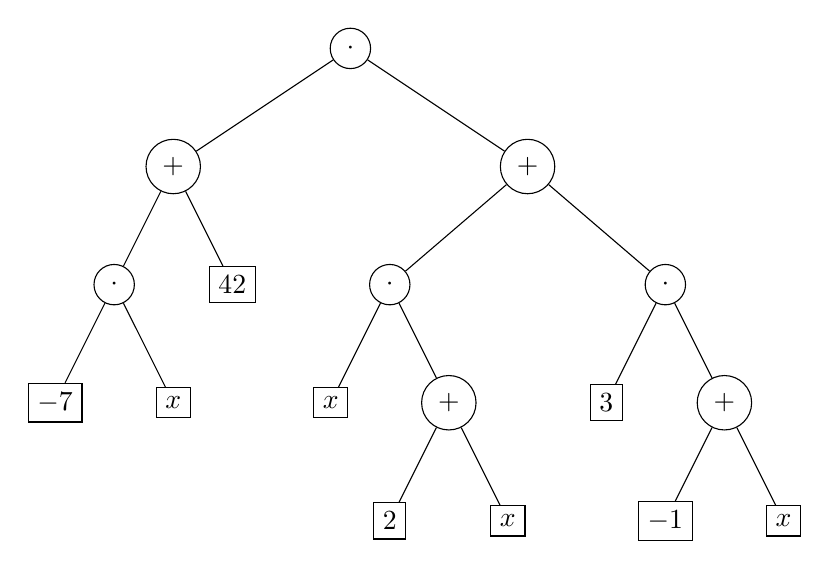
\begin{tikzpicture}
\node [circle,draw] {$\cdot$}
  child {
    node [circle,draw,xshift=-15mm] {$+$}
    child {
      node [circle,draw] {$\cdot$}
      child {node [draw]{$-7$}}
      child {node [draw]{$x$}}
    }
    child {node [draw] {$42$}}
  }
  child {
    node [circle,draw,xshift=15mm] (M) {$+$}
    child {
      node [circle,draw,xshift=-10mm]{$\cdot$}
      child {node [draw]{$x$}}
      child {
        node [circle,draw]{$+$}
        child {node [draw] {$2$}}
        child {node [draw] {$x$}}
        }
      }
    child {
      node [circle,draw,xshift=10mm]{$\cdot$}
      child {node [draw] {$3$}}
      child {
        node [circle,draw] {$+$}
        child {node [draw] {$-1$}}
        child {node [draw] {$x$}}
        }
    }
  };
\end{tikzpicture}
\end{center}
\caption{Il polinomio $P = \enclose{(-7)\cdot x + 42}\cdot(x\cdot (2+x) + 3\cdot(-1+x))$
rappresentato come albero di valutazione.}
\label{fig:49389}%
\end{figure}
Le espressioni polinomiali possono essere sommate e moltiplicate tra loro 
per ottenere nuove espressioni. 
Come comoda notazione si utilizzano le potenze intere per 
denotare un prodotto ripetuto $n$ volte: $x^n = x\cdots x$.

Diremo che due espressioni sono \emph{equivalenti} se è possibile trasformare 
una nell'altra utilizzando le proprietà valide negli anelli abeliani: 
proprietà associativa 
e commutativa per somma e prodotto, proprietà distributiva, elementi 
neutri $1\cdot x = x$, $0 + x = x$.
Inoltre se un ramo dell'espressione non contiene la variabile $x$ è possibile valutare 
(nell'anello $A$) le operazioni e sostituire l'intero ramo con il 
risultato di tali operazioni (e viceversa).

In particolare se abbiamo una qualunque espressione possiamo sviluppare tutti i prodotti
mediante la proprietà distributiva e poi riassociare i termini 
con le stesse potenze di $x$, ad esempio:
\begin{align*}
P &= \enclose{(-7)\cdot x+42}\cdot(x\cdot (2 + x)
+ 3\cdot(-1+x))\\
&= \enclose{(-7)\cdot x + 42}\cdot (2x+x^2-3+3x) \\
% (42-7x)  *  (-3 + 5x + x^2)
&= 126 + 231 x + 7 x^2 - 7 x^3
\end{align*}
In generale si otterrà una espressione polinomiale che diremo 
essere in \emph{forma canonica}:
\[
  P = a_0 + a_1 x + a_2 x^2 + \dots + a_n x^n
       = \sum_{k=0}^n a_k x^k.
\]
Dunque ogni espressione polinomiale è equivalente ad una 
espressione polinomiale in forma canonica. 

Se due espressioni polinomiali sono equivalenti 
diremo che rappresentano lo stesso \emph{polinomio}%
\mymargin{polinomio}%
\index{polinomio}.
Se $A$ è un anello denoteremo con 
$A[x]$ \index{$\KK[x]$}\index{$A[x]$}%
l'insieme di tutti i polinomi con coefficienti in $A$ e variabile $x$. 
Formalmente $A[x]$ è il quoziente dell'insieme 
di tutte le espressioni polinomiali rispetto alla relazione di equivalenza
che abbiamo appena definito. 
Possiamo fare la somma e il prodotto di polinomi e queste operazioni 
rendono $A[x]$ anch'esso un anello.

Più esplicitamente se $P$ e $Q$ sono polinomi in forma canonica
\[
  P = \sum_{k=0}^n a_k x^k, \qquad Q = \sum_{k=0}^m b_k x^k
\]
si avrà:
\[
  P + Q = \sum_{k=0}^{N} (a_k+b_k) \cdot x^k
\]
dove $N$ è il più grande tra $n$ e $m$ e si intende che $a_k=0$ per $k>n$ e 
$b_k=0$ per $k>m$.
Se $t\in A$ avremo:
\[
  t P = \sum_{k=0}^n (ta_k)\cdot x^k.
\]
Per quanto riguarda il prodotto si avrà invece:
\begin{align*}
  P\cdot Q
  &= \enclose{\sum_{k=0}^n a_k x^k}\cdot \enclose{\sum_{j=0}^n b_j x^j}
  = \enclose{\sum_{k=0}^n a_k \enclose{\sum_{j=0}^m b_j x^j} x^k} \\
  &= \enclose{\sum_{k=0}^n \sum_{j=0}^m a_k b_j x^{j+k}}
  = \sum_{s=0}^{m+n} \enclose{\sum_{j=0}^s a_j b_{s-j}} x^s.
\end{align*}

Le formule per la somma e il prodotto dei polinomi in forma canonica 
possono essere applicate ad ognuna delle proprietà di anello per dimostrare
che polinomi equivalenti hanno la stessa forma canonica e che quindi 
due espressioni polinomiali sono equivalenti se e solo se i coefficienti 
della loro forma canonica coincidono.
In pratica i polinomi a coefficienti in $A$ sono 
rappresentati dai coefficienti delle loro forme canoniche che 
non sono altro che sequenze finite:
\begin{align*}
  A[x] 
  &= \{\sum_{k=0}^n a_k x^k\colon a_k\in A, n\in \NN\}\\
  &\approx A^\NN_c 
  = \ENCLOSE{\vec a \in A^\NN\colon \ENCLOSE{k\in \NN\colon \vec a(k)\neq 0} \text{ è finito}}.  
\end{align*}

Se il polinomio $P$ si scrive in forma canonica
\[
  P = \sum_{k=0}^n a_k x^k
\]
se $n>0$ possiamo supporre che il coefficiente $a_n$ sia diverso da $0$ 
perché altrimenti potremmo rimuovere il termine corrispondente e ridurci 
ad una somma di $n-1$ termini. 
In tal caso diremo che il polinomio $P$ ha \emph{grado}%
\mymargin{grado}%
\index{grado} $n$.
\index{polinomio!grado}%
\index{grado!polinomio}% 
Se $n=0$ diremo anche che il polinomio è costante.
Se $n=0$ e $a_n=0$ diremo che $P$ è il polinomio \emph{nullo}.
I polinomi costanti non nulli hanno grado pari a $0$, mentre il polinomio nullo, 
per convenzione, diremo avere grado $-\infty$ (questa definizione ha senso se si pensa 
al grado di un polinomio come al più piccolo numero per cui tutti i coefficienti di
indice maggiore a lui sono nulli).

Finora abbiamo definito il polinomio come una classe di equivalenza di 
espressioni polinomiali. 
Se prendiamo una espressione $P$ e al posto della variabile $x$ 
mettiamo un elemento $a$ dell'anello $A$ (o di qualunque anello che estende 
$A$) allora possiamo valutare tutte le operazioni (somme e prodotti) ed 
ottenere un risultato nell'anello scelto: il risultato 
ottenuto si indica con $P(a)$ (stessa notazione utilizzata per le funzioni).
Se $P$ è un polinomio nella variabile $x$ la funzione $x\mapsto P(x)$ 
può essere chiamata \emph{funzione polinomiale}%
\mymargin{funzione polinomiale}%
\index{funzione!polinomiale} e si indica usualmente 
con con lo stesso nome $P$ dato al polinomio. Sarà il contesto a dirci 
se con $P$ si intende il polinomio (l'espressione) o la funzione.

Come già anticipato è utile tenere separato il concetto di polinomio da quello di 
funzione polinomiale in quanto lo stesso polinomio può essere valutato su diversi 
anelli (ad esempio nel corso di geometria si potrà sostituire
la variabile $x$ di un polinomio con una matrice, 
e nell'ultimo capitolo di questi appunti 
sostituiremo la $x$ con un operatore differenziale).

Proseguiremo con la trattazione dei polinomi 
nel capitolo~\ref{ch:ancora_polinomi}.

\subsection{coefficienti binomiali}
\label{ch:binomiale}

Capiterà spesso di imbattersi in alcuni polinomi particolari, che vengono 
a volte chiamati \emph{prodotti notevoli}%
\mymargin{prodotti notevoli}%
\index{prodotto!notevole}. 
Di fondamentale iportanza quelli di grado 2:
\[
  (x+1)\cdot(x-1) = x^2-1, \qquad (x+1)^2 = x^2+2x + 1.
\]
Ma anche quelli di grado $n$:
\[
  (x-1)\cdot \sum_{k=0}^{n-1} x^k
  = \sum_{k=0}^{n-1} x^{k+1} - \sum_{k=0}^n x^k = x^n - 1
\]
e, mettendo $-x$ al posto di $x$ e cambiando di segno:
\[
  (x+1)\cdot \sum_{k=0}^{n-1} (-1)^k x^k
  = 1 + (-1)^n x^n.
\]

Le potenze del binomio $x+1$ sono decisamente rilevanti. 
Se scriviamo il polinomio $(x+1)^n$ in forma canonica:
\[
  (x+1)^n = \sum_{k=0}^n a_k x^k  
\]
saremmo interessati a calcolare il valore
dei coefficienti $a_k$. 
Innanzitutto gli diamo un nome: questi coefficienti vengono chiamati 
\emph{coefficienti binomiali}%
\mymargin{coefficienti binomiali}%
\index{coefficienti binomiali}
\index{binomio!coefficienti}%
e si denotano nel modo seguente:%
\mynote{%
I coefficienti binomiali nell'ambito del calcolo combinatorio 
vengono anche chiamati \emph{combinazioni}
e denotati con il simbolo $C_{n,k} = {n \choose k}$.
La coincidenza tra le combinazioni e i coefficienti binomiali 
è espressa nel teorema~\ref{th:combinatoria}.
}%
\[
    a_k = {n \choose k}.
\]

Non è difficile convincersi che se sviluppiamo il binomio $(x+y)^n$
si ottengono gli stessi coefficienti dunque
in generale vale la seguente formula per la \emph{potenza del binomio}%
\mymargin{potenza del binomio}%
\index{potenza!del binomio}:
\index{binomio!potenza}% 
\begin{equation*}
  (x+y)^n = \sum_{k=0}^n {n \choose k} x^k y^{n-k}. 
\end{equation*}

Per determinare il valore effettivo dei coefficienti 
binomiali si utilizza usualmente il seguente.
  
\begin{theorem}[triangolo di Tartaglia]
\mymark{*}%
\label{th:tartaglia}%
Per ogni $n\in \NN$ e $k \in \NN$ con $1 \le k \le n$ si ha
\[
  {n+1 \choose k} =
      {n \choose k-1} + {n \choose k}
\]
mentre
\[
  {n+1 \choose 0} = 1 = {n+1 \choose n+1}
\]
\end{theorem}
  %
  \begin{proof}
  Infatti si ha 
  \begin{align*}
    \sum_{k=0}^{n+1} {n+1 \choose k} x^k
    &= (1+x)^{n+1} 
    = (1+x)\cdot \sum_{k=0}^n {n \choose k} x^k \\
    &= \sum_{k=0}^n {n\choose k} x^k 
    + \sum_{k=0}^n {n\choose k} x^{k+1}\\
    &= \sum_{k=0}^n {n\choose k} x^k 
    + \sum_{k=1}^{n+1} {n\choose k-1} x^{k}\\
    &= {n\choose 0} x^0 
      + \sum_{k=1}^n \Enclose{{n\choose k} + {n\choose k-1}} x^k
      + {n \choose n} x^{n+1}.
    \end{align*}
  Per l'unicità della forma canonica dei polinomi 
  i coefficienti corrispondenti devono essere uguali e quindi 
  troviamo
  \[
  {n+1 \choose 0} = {n \choose 0}, \qquad 
  {n+1 \choose k} = {n \choose k} + {n \choose k-1}, \qquad 
  {n+1 \choose n+1} = {n \choose n}.
  \]

  Si può facilmente verificare che  ${0 \choose 0} = 1$ 
  e questo conclude la dimostrazione.
  \end{proof}
  
  In base al teorema precedente i coefficienti binomiali si possono
  elencare come nella tabella~\ref{tab:binomiali}:
  ogni riga inizia e finisce con il numero $1$
  e ogni termine intermedio coincide con la somma dei
  due termini nella riga precedente sopra e
  a sinistra del numero considerato.
  
  \begin{table}
  \begin{tabular}{c|ccccccccc}
  $\displaystyle{n \choose k}$& 0 & 1 & 2 & 3 & 4 & 5 & 6 & $k$ &\\ \hline
    0 & 1 &   &   &   &   &   &   & &\\
    1 & 1 & 1 &   &   &   &   &   & &\\
    2 & 1 & 2 & 1 &   &   &   &   & &\\
    3 & 1 & 3 & 3 & 1 &   &   &   & &\\
    4 & 1 & 4 & 6 & 4 & 1 &   &   & &\\
    5 & 1 & 5 & 10& 10& 5 & 1 &   & &\\
    6 & 1 & 6 & 15& 20& 15& 6 & 1 & &\\
  $n$ &$\vdots$&&   &   &   &   &   & $\ddots$ &
  \end{tabular}
  \caption{Il triangolo di Tartaglia (o di Pascal):
  ogni numero è la somma dei due numeri che si trovano 
  nella riga precedente sopra e immediatamente a sinistra.}
  \label{tab:binomiali}
  \end{table}
  
  \begin{theorem}[formula per i coefficienti binomiali]
  \mymark{***}%
  Se $n\in \NN$ e $k\in \NN$, $k\le n$
  si ha 
  \[
  {n \choose k}  
  = \frac{n!}{k!(n-k)!}.  
  \]
  \end{theorem}
  %
  \begin{proof}
  Lo dimostriamo per induzione su $n$.
  Per $n=0$ sappiamo che ${0 \choose 0} = 1$ che 
  è ugule a $\frac{0!}{0!0!}$.
  Utilizziamo il teorema~\ref{th:tartaglia}.
  Se $k=0$ o $k=n$ sappiamo che ${n \choose k}=1$ che coincide 
  con la formula enunciata. 
  Per gli altri casi, supponendo per induzione che la formula sia 
  vera per un certo $n\in \NN$ si ha: 
  \begin{align*}
   {n+1 \choose k} 
   &= {n \choose k} + {n \choose k-1}
   =  \frac{n!}{k!(n-k)!} + \frac{n!}{(k-1)!(n-k+1)!} \\
   &= \frac{n!(n-k+1) + n! k}{k!(n-k+1)!}
   = \frac{n!(n+1)}{k!(n+1-k)!} \\
   &= \frac{(n+1)!}{k!(n+1-k)!}
  \end{align*}
  che è quanto dovevamo dimostrare.
\end{proof}

Si osservi che risulta, per ogni $n\in \NN$:
\[
  {n \choose 1} = {n \choose n-1} = n.
\]
  
\begin{exercise}
  Provare che
  \[
   \sum_{k=0}^n {n \choose k} = 2^n.
  \]
\end{exercise}  


\subsection{scomposizione dei polinomi}

\begin{theorem}[divisione di Euclide]
  \label{th:divisione_polinomi}%
  \index{divisione tra polinomi}%
  \index{polinomio!divisione}%
  \index{polinomio!algoritmo di Euclide}%
  \index{Euclide!algoritmo di divisione}%
  \index{algoritmo!di Euclide}%
  Se $\KK$ è un campo,
  dati due polinomi $P$ e $S$ in $\KK[x]$ con $S\neq 0$ è possibile
  trovare, in modo unico, due polinomi $Q$ (quoziente)
  e $R$ (resto) in $\KK[x]$ con $\deg R < \deg S$
  tali che:
  \[
    P = Q \cdot S + R.
  \]
  \end{theorem}
  %
  \begin{proof}
  \emph{Passo 1:} supponiamo che sia $\deg P < \deg S$.
  In questo caso basta prendere $Q=0$ e $R=P$.
  
  \emph{Passo 2:} supponiamo che sia $\deg P \ge \deg S$.
  Poniamo $N=\deg P$ e $M=\deg S$.
  Sia $a_N\neq 0$ il coefficiente del termine di grado massimo
  di $P$ e $b_M\neq 0$ il coefficiente di grado massimo
  del polinomio $S$.
  E' allora facile verificare che il polinomio
  \[
  \frac{a_N}{b_M} \cdot x^{N-M}\cdot S
  \]
  ha lo stesso grado di $P$ e il suo coefficiente di grado
  massimo è uguale ad $a_N$ in quanto è il prodotto di
  $a_N/b_M$ per $b_M$.
  Dunque il polinomio
  \[
   P_1 = P - \frac{a_N}{b_M} \cdot x^{N-M}\cdot S
  \]
  ha grado strettamente inferiore a $P$.
  Possiamo ora supporre, mediante un ragionamento induttivo
  su $\deg P - \deg S$
  che per il polinomio $P_1$ il risultato del teorema sia
  valido cioè
  che esistano, dei polinomio $Q_1$ e $R$
  con $\deg R < \deg S$ tali che
  \[
    P_1 = Q_1 \cdot S + R.
  \]
  Il caso base del ragionamento induttivo,
  $\deg P = \deg S$, è garantito dal passo 1.
  Avremo allora:
  \begin{align*}
    P &= P_1 + \frac{a_N}{b_M} x^{N-M}\cdot S\\
      &= Q_1 \cdot S + R_1 + \frac{a_N}{b_M} x^{N-M}\cdot S\\
      &= (\frac{a_N}{b_M} x^{N-M} + Q_1) \cdot S + R_1.
  \end{align*}
  Posto quindi
  \[
   Q = \frac{a_N}{b_N} x^{N-M} + Q_1
  \]
  il risultato è dimostrato.
  
  \emph{Passo 3:} dimostriamo che $Q$ e $R$ sono unici. Se infatti avvessimo 
  \[
    P = Q_1 S + R_1 = Q_2 S + R_2   
  \]
  con $\deg R_1<\deg S$ e $\deg R_2 < \deg S$ si avrebbe 
  \[
  (Q_2 - Q_1) S = R_1 - R_2.    
  \]
  Se fosse $Q_2 \neq Q_1$ il polinomio al lato sinistro avrebbe grado non inferiore al grado di 
  $S$ mentre il lato destro ha certamente grado minore di $S$.
  Dunque $Q_2=Q_1$ ma allora il lato sinistro è nullo e quindi anche il lato destro deve 
  esserlo: $R_2=R_1$.
  \end{proof}
  
  La dimostrazione del teorema precedente fornisce anche un
  algoritmo, chiamato \emph{algoritmo di Euclide},
  per eseguire la divisione (con resto) tra polinomi.
  Lo sperimentiamo nel seguente esercizio.
  
  \begin{exercise}
  Sia $P = x^4-3 x^2 + 2x + 1$ e $S = x^2-1$.
  Eseguire la divisione con resto cioè:
  trovare $Q$ ed $R$ con $\deg R < \deg S$ tali che
  \[
  P = Q \cdot S + R.
  \]
  \end{exercise}
  %
  \begin{proof}[Svolgimento.]
  Il rapporto tra i termini di grado massimo di
  $P$ e $S$ è $x^4/x^2 = x^2$.
  Dunque consideriamo come primo monomio $x^2$.
  Si ha
  \begin{align*}
    P_1
    &= P - x^2 \cdot S
    = x^4-3x^2+2x+1 - x^4+x^2 \\
    &= -2x^2+2x+1.
  \end{align*}
  Ripetiamo il procedimento con $P_1$ al posto di $P$.
  Il rapporto tra i termini di grado massimo di $P_1$ e $S$
  è il monomio $-2$. Si ha
  \[
    P_2 = P_1 - (-2) S = -2x^2 + 2x + 1 + 2x^2 - 2 = 2x -1.
  \]
  Visto che $\deg P_2 < \deg S$ la divisione termina e
  si pone $R = 2x-1$.
  Si ha quindi $Q = x^2 - 2$ (la somma dei monomi trovati)
  e risulta:
  \[
    P = (x^2 - 2)\cdot S + 2x -1.
  \]
  \end{proof}
  
  \begin{theorem}[Ruffini]
  \label{th:Ruffini}%
  \index{teorema!di Ruffini}%
  \index{Ruffini}%
  Sia $P\in \KK[x]$ un polinomio non nullo.
  Se $x_0 \in \KK$ è tale che $P(x_0)=0$
  allora esiste un polinomio $Q$ con $\deg Q = (\deg P) - 1$
  tale che
  \[
    P = (x-x_0)\cdot Q.
  \]
  \end{theorem}
  %
  \begin{proof}
  In base al teorema precedente si può fare la divisione tra
  $P$ e $S = x - x_0$ per ottenere un polinomio $Q$ e un resto
  $R$ con $\deg R < 1$ tali che
  \[
    P = (x-x_0)\cdot Q + R.
  \]
  Siccome $\deg R < 1$ si ha in effetti che $R=c\in \KK$
  è un polinomio costante e dunque
  \[
    P = (x-x_0) \cdot Q + c
  \]
  ma valutando $P$ in $x=x_0$ si scopre che
  \[
   P(x_0) = 0\cdot Q(x_0) + c = c
  \]
  dunque $c=P(x_0) = 0$.
  \end{proof}
  
  Possiamo ora chiederci se polinomi diversi corrispondono
  a funzioni polinomiali diverse.
  In generale questo non è vero, se ad esempio prendessimo
  come campo $\KK=\ZZ_2 = \ENCLOSE{0,1}$, un campo finito
  in cui poniamo $1+1=0$ scopriremmo che la funzione polinomiale
  $P(x) = x^2+x$ è identicamente nulla in quanto $0^2+0=0$
  e $1^2+1=1+1=0$ in questo campo.
  Ma nei casi che interessano a noi $\KK=\RR$ o $\KK=\CC$
  questo problema non si presenta e si potrà quindi identificare
  ogni polinomio con la corrispondente funzione polinomiale.
  Per avere questa garanzia ci servono i seguenti risultati.
  
  \begin{theorem}[principio di annullamento dei polinomi]
  \label{th:annullamento_polinomi}%
  \index{principio!di annullamento dei polinomi}%
  Sia $P\in \KK[x]$ un polinomio non nullo di grado $n$.
  Allora la funzione polinomiale associata a $P$
  si annulla in al più $n$ punti distinti di $\KK$.
  
  In particolare se un polinomio si annulla in infiniti
  punti distinti allora tale polinomio è certamente nullo.
  \end{theorem}
  %
  \begin{proof}
  Dimostriamo per induzione su $n$ che se un polinomio
  $P$ di grado non superiore a $n$ si annulla in $n+1$
  punti distinti $x_1, \dots, x_{n+1}\in \KK$ allora
  $P=0$.
  
  Se $n=0$ il polinomio $P$ è costante ma si annulla
  in un punto e quindi è il polinomio nullo.
  Se $n>0$ per il teorema di Ruffini applicato al
  punto $x_{n+1}$ sappiamo che esise un polinomio $Q$
  di grado inferiore ad $n$ per cui si ha
  \[
    P = (x-x_{n+1}) \cdot Q
  \]
  sostituendo $x=x_k$ con $k\le n$ si ha $x_k-x_{n+1}\neq 0$
  e quindi
  \[
    Q(x_k) = \frac{P(x_k)}{x_k-x_{n+1}} = 0.
  \]
  Dunque $Q$ si annulla nei punti $x_1, \dots, x_n$
  e, per ipotesi induttiva, scopriamo che $Q$ deve
  essere nullo. Di conseguenza anche $P$ è nullo.
  \end{proof}
  
  Se $\KK$ è un insieme infinito (come nei casi $\KK=\RR$ o $\KK=\CC$)
  si trova che
  se a due polinomi $P$, $Q$ corrisponde
  la stessa funzione polinomiale:
  \[
    P(x) = Q(x) \qquad \text{per ogni $x\in \KK$}
  \]
  allora $P$ e $Q$ sono lo stesso polinomio $P=Q$
  in quanto la differenza $P-Q$ si annulla in tutti i punti
  di $\KK$ e qualunque sia il suo grado, se $\KK$ è infinito,
  questo ci dice che $P-Q=0$. 
  
  Questo corollario viene spesso enunciato come segue.
  \begin{theorem}[principio di identità dei polinomi]
    Siano $a_k$ e $b_k$ coefficienti nel campo $\KK=\RR$ o $\KK=\CC$.
    Se per ogni $x\in \KK$ si ha 
    \[
       \sum_{k=1}^n a_k x^k = \sum_{k=1}^m b_k x^k
    \]
    allora $m=n$ e $a_k=b_k$ per ogni $k=0, \dots, n$.
  \end{theorem}
  %
  \begin{proof}
  Facendo la differenza dei due lati dell'uguaglianza si ottiene 
  che una espressione polinomiale si annulla identicamente. 
  Allora per il teorema~\ref{th:annullamento_polinomi} tale espressione 
  rappresenta il polinomio nullo e di conseguenza tutti i coefficienti, 
  che sono dati dalla differenza $a_k-b_k$, devono essere nulli.
  \end{proof}
  
\begin{example}
L'insieme $\ZZ_2={0,1}$ può essere reso un campo 
se si definisce la somma e il prodotto come sui 
numeri naturali prendendo però sempre il resto 
modulo $2$: $0+0=1+1=0$, $0+1=1+0=1$, $0\cdot 0
=1\cdot 0 = 0\cdot 1 = 0$, $1\cdot 1=1$.
Si può verificare che effettivamente $\ZZ_2$ 
è un campo.
Il polinomio $P = x^2+x$ risulta annullarsi sia 
per $x=0$ che per $x=1$, ma non è il polinomio nullo.
\end{example}

\section{cardinalità}
\label{sec:cardinali}

\begin{definition}[cardinalità]
  Diremo che due insiemi $A$ e $B$ hanno la stessa \emph{cardinalità}%
\mymargin{cardinalità}%
\index{cardinalità} 
  (oppure sono \emph{equipotenti}) 
  \index{equipotenza}%
  \index{insiemi!equipotenti}%
  \index{insieme!equipotente}%
  se esiste una funzione bigettiva $f\colon A \to B$.
  Scriveremo in tal caso:
  \[
    \# A = \# B.  
  \] 
  Se esiste una funzione iniettiva $f\colon A\to B$ significa che 
  $A$ ha la stessa cardinalità di un sottoinsieme di $B$ (in quanto $f\colon A \to f(A)$
  risulta essere bigettiva). Scriveremo in tal caso:
  \[
    \# A \le \#B.
  \]
\end{definition}

Intuitivamente se due insiemi hanno la stessa cardinalità 
significa che hanno lo stesso numero di elementi.
Ma la precedente definizione riesce a catturare tale concetto senza dover 
ricorrere al concetto di numero. 
Questo ha il vantaggio di rendere questa definizione applicabile 
a qualunque insieme, anche con \emph{infiniti} elementi.

Si osservi che non abbiamo dato una definizione di $\#A$ e quindi non stiamo 
definendo cos'è la cardinalità di un insieme ma stiamo soltanto definendo 
una relazione tra insiemi che 
denotiamo, impropriamente, utilizzando una uguaglianza: $\#A = \#B$.

E' ovvio che $\#A = \#A$ in quanto l'identità $\id_A$ è bigettiva.
E' anche chiaro che se $\#A = \#B$ e $\#B = \#C$ allora $\#A = \#C$ in quanto 
componendo tra loro due funzioni bigettive si ottiene ancora una funzione 
bigettiva. 
Infine se $\#A = \#B$ allora $\#A \le \#B$ (in quanto le funzioni bigettive 
sono iniettive) ed è chiaro che se $\#A \le \#B$ e $\#B \le \#C$ allora 
$\#A\le \#C$ (in quanto composizione di funzioni iniettive è iniettiva).

Possiamo definire il simbolo inverso $\#A \ge \#B$ 
come $\#B\le \#A$.
Ovviamente se $A\subset B$ si ha $\#A \le \#B$.
Se $B\neq \emptyset$ 
il seguente teorema ci dice che $\#A \ge \#B$ 
è equivalente a dire che 
esiste $f\colon A \to B$
surgettiva. 
%
\begin{theorem}\label{th:95444}
  Sia $B\neq \emptyset$.
  Esiste $f\colon A\to B$ surgettiva 
  se e solo se esiste $g\colon B\to A$ iniettiva.
\end{theorem}
% 
\begin{proof}
Da un lato se esiste $g\colon B\to A$ iniettiva, allora $g$ è una bigezione 
tra $B$ e $g(B)$. La funzione inversa $f\colon g(B) \to B$ 
\mynote{Questa funzione $f$ si chiama 
\emph{inversa sinistra}
\index{inversa!sinistra}%
di $g$ in quanto si ha $f(g(y))=y$ per ogni $y\in B$}
può essere estesa a tutto $A$ fissando un valore qualunque 
(questo si può fare se $B$ non è vuoto) nei punti di $A\setminus g(B)$
ottenendo quindi una funzione surgettiva da $A$ in $B$.
D'altro lato se esiste una funzione $f\colon A\to B$ surgettiva,
per ogni $b\in B$ l'insieme $f^{-1}(\ENCLOSE{b})$ non è mai 
vuoto e quindi è chiaro che debba esistere 
una funzione $g\colon B\to A$ tale che $g(b)$ è un qualunque elemento 
di tale insieme
\mynote{Questa funzione $g$ si chiama 
\emph{inversa destra} 
\index{inversa!destra}%
di $f$ 
in quanto $f(g(y))=y$ per ogni $y\in B$}
(qui si utilizza l'assioma~\ref{axiom:AC} discusso più sotto). 
Chiaramente $g$ è iniettiva.
\end{proof}

Nella dimostrazione del teorema precedente abbiamo utilizzato il seguente assioma 
della teoria degli insiemi che, sorprendentemente, non è conseguenza degli assiomi 
che abbiamo già introdotto finora.

\begin{axiom}[della scelta]%
  \label{axiom:AC}%
  \index{assioma!della scelta}%
  \index{scelta!assioma della}%
  \index{AC}%
  Sia $F\colon A \to \mathcal P(B)$
  una funzione tale che $F(a)\neq \emptyset$ 
  per ogni $a\in A$. Allora esiste una funzione
  $f\colon A \to B$ tale che $f(a)\in F(a)$
  per ogni $a\in A$.
\end{axiom}

L'assioma della scelta (denotato spesso con \emph{$AC$}%
\mymargin{$AC$}%
\index{AC}, \emph{axiom of choice})
è un assioma per certi versi controverso
e alcuni matematici preferiscono non utilizzarlo nelle loro dimostrazioni.
Il sistema formale che definisce la teoria degli insiemi senza 
introdurre l'assioma della scelta 
si chiama \emph{$ZF$}%
\mymargin{$ZF$}%
\index{ZF} (Zermelo-Fraenkel) mentre 
se si aggiunge l'assioma della scelta (choice) la teoria si chiama 
\emph{$ZFC$}%
\mymargin{$ZFC$}%
\index{ZFC}.

Grazie all'assioma della scelta è anche possibile dimostrare 
che dati due insiemi $A$ e $B$ le loro cardinalità
si possono confrontare: $\#A\le \#B$ oppure 
$\#B\le \#A$. 
La dimostrazione però diventa complicata e va oltre i nostri scopi.

\begin{theorem}
  \label{th:cardinale_totale}%
  Se $A$ e $B$ sono insiemi qualunque si ha $\#A\le \#B$ oppure $\#B\le \#A$.
\end{theorem}

Il seguente teorema dimostra invece la proprietà antisimmetrica 
della relazione tra cardinalità. 
E' probabilmente il primo vero teorema 
(con dimostrazione decisamente non banale) 
che andiamo a dimostrare.

\begin{theorem}[Cantor-Bernstein]%
  \label{th:cantor_bernstein}%
  \index{teorema!di Cantor-Bernstein}%
  \index{Cantor-Bernstein!teorema di}%
  Se $\#A \le \#B$ e $\#B \le \#A$ allora $\#A = \#B$.
\end{theorem}
%
\begin{figure}
  \centering
  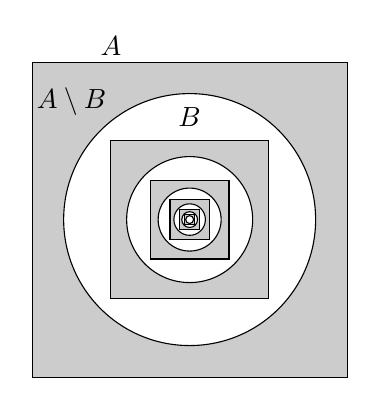
\begin{tikzpicture}
    \foreach \x in {1,0.5,0.25,0.25*0.5,0.25*0.25,0.25*0.25*0.5} {
      \path[draw,fill=black!20] (2*\x,2*\x)--(-2*\x,2*\x)--(-2*\x,-2*\x)--(2*\x,-2*\x)--cycle;
      \draw[fill=white] (0,0) circle (1.6*\x);
    };
    \node at (-1.0,2.2) {$A$};
    \node at (-1.5,1.5) {$A\setminus B$};
    \node at (0,1.3) {$B$};
%    \node at (-0.75,0.75) {$$};
  \end{tikzpicture}
  \caption{
  Nella dimostrazione del teorema di Cantor-Bernstein
  $A$ è rappresentato da un quadrato e $B$ da un cerchio contenuto
  in $A$. L'immagine di $A$ in $B$ è rappresentata da un quadrato contenuto
  in $B$ e così via. La parte ombreggiata è l'insieme $D$.
  }
  \label{fig:omotetia}
\end{figure}
%
\begin{proof}
Per ipotesi sappiamo che esiste
$g\colon B\to A$ iniettiva. 
Posto $B'=g(B)$ risulta che $g\colon B\to B'$ è bigettiva.
Ma allora dimostrare che esiste una bigezione tra $A$ e $B$ 
è equivalente a dimostrare che esiste una bigezione tra 
$A$ e $B'$. 
Dunque senza perdere di generalità, sostituendo $B'$ a $B$ 
possiamo supporre che sia $B\subset A$.

Essendo per ipotesi $\#A \le \#B$ esiste $f\colon A \to B$ iniettiva.
Intuitivamente l'idea è quella di definire l'insieme
\[
 D = (A\setminus B)  
 \cup f(A\setminus B) 
 \cup f(f(A\setminus B)) 
 \cup \dots
\]
e di definire la bigezione $\phi \colon A \to B$ 
utilizzando $f$ sull'insieme $D$ e lasciando fisso
il resto.

Per farlo in maniera rigorosa
consideriamo la famiglia di insiemi 
$\F = \{X \subset A \colon X \supset A \setminus B, f(X) \subset X\}$ 
e definiamo $D = \bigcap \F$.
Osserviamo che $A \in \F$ quindi $\F\neq \emptyset$.
Abbiamo in pratica definito $D$ come il più piccolo 
sottoinsieme di $A$ che viene mandato in se stesso da $f$.

E' facile verificare che $f(D) \subset D$ infatti dato $x\in D$ per ogni $X\in \F$ deve essere $x\in X$ ma allora $f(x) \in X$ (per come è definito $\F$), dunque $f(x) \in D$. 
In modo analogo si dimostra che $D\supset A\setminus B$ e dunque concludiamo che $D\in \F$.

Verifichiamo ora che $f(D)=D\cap B$. Da un lato se $x\in D$ allora
$f(x) \in f(D)\subset D$ e $f(x)\subset f(A)\subset B$ da cui $f(x) \in D\cap B$.
Dall'altro lato se $y\in D \cap B$ e non fosse $y \in f(D)$
allora potremmo considerare l'insieme $X=D\setminus\{y\}$
e osservare che $X\in \F$.
Infatti in primo luogo $X \supset A \setminus B$ in quanto $D$ ha questa proprietà e $y \in B$.
Inoltre dato qualunque $x \in X$ visto che $X\subset D$ allora
$f(x) \in f(D)$ e, per ipotesi,
$y\not \in f(D)$ dunque $f(x)\neq y$ da cui $f(x) \in X$.
Dunque $X\in \F$ ma allora dovrebbe essere $D\subset X$ mentre
per costruzione abbiamo $y\in D$ ma non in $X$.

% Avendo visto che $f(D)=D\cap B$ possiamo facilmente
% osservare che $f(A\setminus D) \subset A \setminus D$.
% Infatti $f(A\setminus D)\subset f(A)=B$ e quindi
% $f(A\setminus D)\cap D \subset D \cap B = f(D)$
% ma essendo $f$ iniettiva si deve avere
% $f(A\setminus D) \cap f(D)=\emptyset$.

Possiamo allora definire $\phi \colon A \to B$
\[
\phi(x) =
\begin{cases}
   f(x) & \text{se $x\in D$}, \\
   x & \text{altrimenti.}
\end{cases}
\]
Chiaramente $\phi$ è iniettiva in quanto $f$ è iniettiva e manda $D$ in $D$
e l'identità è iniettiva e manda $A\setminus D$ in $A\setminus D$.

Per dimostrare che $\phi$ è suriettiva consideriamo qualunque $y \in B$.
Se $y\not \in D$ allora $\phi(y)=y$.
Se invece $y\in D$ essendo $y\in D\cap B = f(D)$ esisterà $x\in D$ tale
che $\phi(x) = f(x) = y$.
\end{proof}

Ricordiamo il teorema~\ref{th:cardinali_finiti}
che ci dice che $A$ è un insieme finito se e solo se 
esiste $n\in\NN$ 
tale che $\#A = #[n]$ dove abbiamo posto $[n]=\ENCLOSE{k\in \NN, k<n}
=\ENCLOSE{0,\dots,n-1}$.
Ora possiamo osservare che $\#A=n$ è una abbreviazione di $\#A = \#[n]$.

La cardinalità di $\NN$ viene a volte indicata con il simbolo
\index{$\aleph_0$}%
\index{aleph}%
$\aleph_0$ dunque potremo scrivere  
\mynote{%
Il simbolo $\aleph$ è la prima lettera dell'alfabeto ebraico 
e si legge \emph{aleph}. \\
Ricordiamo (teorema~\ref{th:unicitaN}) che gli insiemi 
$\NN$ che soddisfano gli assiomi di Peano sono tutti tra loro isomorfi 
e quindi, in particolare, hanno tutti la stessa cardinalità.
Abbiamo già osservato (teorema~\ref{th:esistenza_naturali}) 
che se $A$ è un insieme infinito esiste $N\subset A$
che soddisfa gli assiomi di Peano. 
L'inclusione $N\to A$ è iniettiva e quindi $\aleph_0 = \# \NN \le \# A$
per qualunque $A$ infinito.
In questo senso $\NN$ è il \emph{più piccolo} insieme 
infinito dunque $\aleph_0$ è la più piccola 
cardinalità infinita.

Si potrebbe anche dimostrare che deve esistere una cardinalità $\aleph_1>\aleph_0$
che è la più piccola cardinalità maggiore di $\aleph_0$.
Sappiamo che $\# \mathcal P(\NN)>\# \NN$ ma curiosamente non è possibile dimostrare 
che $\aleph_1 = \# \mathcal P(\NN)$ (questa si chiama \emph{ipotesi del continuo}
\index{ipotesi!del continuo}%
\index{continuo!ipotesi del}%
in quanto vedremo nel teorema~\ref{th:cantor_secondo} che $\# \mathcal P(\NN)=\#\RR$
e l'insieme $\RR$ viene chiamato \emph{continuo} là dove $\NN$ 
viene chiamato \emph{discreto}).
Dunque l'ipotesi del continuo è un ulteriore assioma che potrebbe essere 
aggiunto agli assiomi della teoria degli insiemi: 
non esistono insiemi con cardinalità strettamente compresa tra 
le cardinalità di $\NN$ e di $\mathcal P(\NN)$.
}%
\[
    \# A = \aleph_0, \qquad
    \#A \le \aleph_0, \qquad
    \# A\ge \aleph_0
\]
per significare rispettivamente 
\[
  \# A = \# \NN, \qquad
  \# A \le \# \NN, \qquad
  \# A \ge \# \NN.  
\]
\end{definition}

Abbiamo già osservato che $\NN$ è un insieme infinito e dunque 
anche $\ZZ$, $\QQ$ e $\RR$ sono infiniti.
Per gli insiemi finiti se $A\subset B$ ma $A\neq B$ risulta $\#A < \# B$
in quanto $\#A - \#B = \#(B\setminus A) > 0$. 
Dobbiamo però osservare che lo stesso non vale per gli insiemi infiniti.
In effetti la funzione $s\colon \NN \to \NN$ definita da $s(x)=x+1$
risulta essere una bigezione tra $\NN$ e $\NN\setminus\ENCLOSE{0}$. 
Dunque $\#\NN = \#(\NN\setminus\ENCLOSE{0})$ 
nonostante la differenza tra i due insiemi $\ENCLOSE{0}$ abbia 
cardinalità $1$. 
Anche l'insieme dei numeri pari o l'insieme 
dei quadrati perfetti (come aveva notato già Galileo)
hanno la stessa cardinalità di $\NN$ in quanto le funzioni $n\mapsto 2n$
e la funzione $n\mapsto n^2$ sono iniettive.

Non è difficile trovare una funzione iniettiva da $\ZZ$ in $\NN$
(lo lasciamo per esercizio): questo dimostra che anche $\#\ZZ = \# \NN$.

Cantor dimostra addirittura che $\#\QQ = \#\NN$: 
per farlo utilizza il seguente.

\begin{theorem}[primo metodo diagonale di Cantor]
\label{th:Cantor_primo}%
\index{Cantor!primo metodo diagonale}%
L'insieme $\NN \times \NN$ ha la stessa cardinalità di $\NN$. Di conseguenza
\[
  \# \NN = \# \ZZ = \# \QQ.
  \]
\end{theorem}
%
\begin{proof}[Idea di dimostrazione]
  Numerare le caselle di una scacchiera infinita
  come in Figura~\ref{fig:cantor1}.
  
  Visto che è piuttosto facile trovare una funzione iniettiva 
  da $\QQ$ in $\NN \times \ZZ$ si deduce facilmente che $\#\QQ = \#\NN$.
\end{proof}

\begin{figure}
  \begin{tabular}{c|ccccccc}
   $m$ & $\ddots$ & $\ddots$ & $\ddots$ & $\ddots$ & $\ddots$ & $\ddots$\\
   $\vdots$ & $\ddots$ & $\ddots$ & $\ddots$ & $\ddots$ & $\ddots$ & $\ddots$\\
   3 & 9 & $\nwarrow$ & $\ddots$  & $\ddots$ & $\ddots$ & $\ddots$\\
   2 & 5 & 8 & 12 & $\ddots$  & $\ddots$ & $\ddots$\\
   1 & 2 & 4 & 7 & 11 & $\ddots$  & $\ddots$\\
   0 & 0 & 1 & 3 & 6 & 10 & $\ddots$ \\ \hline
     & 0 & 1 & 2 & 3 & 4 & $\dots$ & $n$
  \end{tabular}
  \caption{
    La numerazione diagonale delle caselle
    di una scacchiera infinita. Si potrebbe verificare
    che il numero presente nella casella di coordinate $(n,m)$
    si scrive come $f(n,m) = \frac{(n+m+1)(n+m)}{2}+m$
    ed è una funzione bigettiva $f\colon \NN\times\NN \to\NN$.}
  \label{fig:cantor1}
\end{figure}

A questo punto si potrebbe pensare che
tutti gli insiemi infiniti siano numerabili.
Invece preso un qualunque insieme (anche infinito)
esiste sempre un insieme con cardinalità maggiore,
come dimostrato nel seguente teorema che è un piccolo gioiello della logica.
In effetti il metodo utilizzato è assimilabile al paradosso del mentitore 
ed è la stessa idea usata nel paradosso di Russell (teorema~\ref{th:Russell}).
\mynote{L'insieme $\mathcal P(A)$ è l'insieme delle parti, 
definito a pag.~\pageref{def:insieme_parti}}%
%
\begin{theorem}[Cantor]%
\index{Cantor!cardinalità dell'insieme delle parti}%
\index{Teorema di!Cantor}%
\label{th:Cantor}%
  Se $A$ è un qualunque insieme allora $\# \mathcal P(A) > \# A$.
\end{theorem}
%
\begin{proof}
  E' chiaro che $\# A \le \#\mathcal P(A)$ in quanto 
  la funzione $f\colon A \to \mathcal P(A)$ definita da $f(x)=\ENCLOSE{x}$
  è ovviamente iniettiva.

  Supponiamo allora per assurdo che esista $f\colon A\to \mathcal P(A)$
  bigettiva e consideriamo l'insieme 
  \[
    C = \ENCLOSE{x\in A \colon x\not\in f(x)}.  
  \]
  Se $f$ fosse surgettiva dovrebbe esistere $c\in A$ tale che $f(c) = C$.
  Possiamo allora chiederci se $c\in C$ e scoprire che, 
  per definizione di $C$ la proposizione $c\in C$ è equivalente 
  a $c\not\in f(c) = C$. 
  Dunque $c\in C \iff c\not\in C$, che è assurdo.
\end{proof}
%
\begin{corollary}[non esiste l'insieme di tutti gli insiemi]
  Se esistesse un insieme $\mathcal U$ (universo) 
  tale che $\forall x\colon x \in U$, allora 
  si avrebbe $\mathcal \P(\mathcal U) \subset \mathcal U$
  contraddicendo il teorema precedente.
\end{corollary}
%
Per quanto riguarda l'insieme $\RR$ si
scopre in effetti che $\#\RR > \#\NN$
(sempre grazie a Cantor, teorema~\ref{th:cantor_secondo})
e si potrebbe dimostrare che effettivamente $\#\RR = \#\mathcal P(\NN)$.

\section{note storiche}

\label{nota:Peano}%
\index{Peano!Giuseppe}%
\emph{Giuseppe Peano} (1858--1932), matematico torinese, contribuì a porre 
i fondamenti della logica matematica. 
La notazione $\exists$ per il quantificatore universale si deve a lui.
La definizione originale di Peano prendeva $1$ come primo numero
naturale ma nella matematica moderna risulta più comodo includere anche $0$ 
tra i numeri naturali, così come si considera il vuoto tra gli insiemi.

\label{nota:Galileo}%
\index{Galileo!Galilei}%
\emph{Galileo Galilei} (1564--1642) osservò che i quadrati 
perfetti: $1,4,9,16,\dots$ sono da un lato una piccola parte 
di tutti i numeri naturali (questi numeri si distanziano 
sempre di più tra loro) ma d'altro canto sono tanti quanti i numeri naturali 
perché la corrispondenza $n\mapsto n^2$ è biunivoca.

\label{nota:Cantor}%
\index{Cantor!Georg}%
\label{nota:Russell}%
\index{Russell!Bertrand}%
\label{nota:Frege}%
\index{Frege!Gottlob}%
La teoria degli insiemi
è stata introdotta da \emph{Georg Cantor} (1845--1918) senza una vera formalizzazione logica
(oggi la chiameremmo \emph{teoria ingenua degli insiemi}).
\emph{Gottlob Frege} (1848--1925) fu il primo matematico che tentò di formalizzare 
la teoria degli insiemi di Cantor. 
Nel 1902 \emph{Bertrand Russell}, avendo letto il lavoro di Frege, 
gli invio una lettera che enunciava il paradosso da lui scovato:
``Mi trovo in completo accordo con lei in tutte le parti essenziali, in particolare
quando lei rifiuta ogni elemento psicologico dando un grande valore
all'ideografia %[Begriffsschrift]
per il fondamento della matematica e della logica formale [\dots] c'è solo
un punto dove ho incontrato una difficoltà [...]''.
La risposta di Frege (22 giugno 1902) è deprimente:
``La sua scoperta della contraddizione mi ha causato una grandissima sorpresa e,
direi, costernazione, perché ha scosso le basi su cui intendevo costruire l'aritmetica.''

\label{nota:Euclide}%
\label{nota:Hilbert}%
\index{Euclide}%
\index{assiomi!di Euclide}%
\index{Hilbert!David}%
\index{geometria euclidea}%
\emph{Euclide} (circa 300 a.C.) ha introdotto il metodo assiomatico in geometria. 
Il suo trattato ``gli Elementi'', è considerato il libro
che in assoluto ha avuto maggiore impatto nella storia della matematica.
Gli assiomi introdotti da Euclide corrispondono alle costruzioni geometriche fatte 
con riga e compasso.
Se consideriamo l'insieme dei punti che possono essere costruiti a partire da 
un insieme finito di punti dati, otteniamo un insieme denso che però 
non è completo. 
E' ben noto, infatti, che tramite riga e compasso non è possibile 
fare la \emph{trisezione dell'angolo} (cioè dividere 
un angolo generico in tre parti uguali)
né la \emph{duplicazione del cubo}
(cioè costruire il lato di un cubo il cui volume sia il doppio di un cubo di dato lato)
né la \emph{quadratura del cerchio} (cioè costruire il lato di un quadrato
con la stessa area di un cerchio di dato raggio).
I primi due problemi richiedono la costruzione delle radici cubiche, mentre 
il terzo problema richiede la costruzione di $\sqrt\pi$.
Tramite la teoria di Galois si è dimostrato che tramite costruzioni con riga e 
compasso si possono costruire solo quei numeri che si possono esprimere 
a partire dai numeri interi utilizzando, oltre alle quattro operazioni, 
l'estrazione di radice quadrata. 
E' facile costruire, ad esempio, la diagonale di un quadrato di dato lato: 
questo corrisponde alla costruzione di $\sqrt 2$.
Ovvio invece che i numeri trascendenti (come $\sqrt\pi$) non possono essere costruiti, visto 
che le operazioni ammissibili non ci fanno uscire dall'insieme dei numeri algebrici.
La costruzione di un poligono regolare inscritto in un cerchio di dato raggio 
è equivalente alla costruzione delle radici complesse $n$-esime dell'unità, ed 
è quindi legato alla costruibilità di particolari numeri algebrici. 
Solo grazie all'apporto di Gauss (1777-1855) c'è stato un avanzamento rispetto alle conoscenze di Euclide 
su quali fossero i poligoni regolari costruibili.
Sorprendentemente 
mentre i poligoni regolari con $7$, $9$, $11$ e $13$ lati non sono costruibili 
con riga e compasso, il poligono regolare con $17$ lati è costruibile
(Gauss-Wentzel). 

Tutta questa discussione dovrebbe rendere chiaro che non è ovvio come si possa 
definire lo spazio geometrico in modo rigoroso 
in modo che risulti essere completo. 
In effetti solo nel 1900 \emph{David Hilbert} (1862--1943) ha dato una definizione assiomatica rigorosa
della geometria euclidea. 
La proprietà di completezza viene catturata da Hilbert mediante un assioma di massimalità:
lo spazio euclideo è un insieme di punti che soddisfano certi assiomi 
(gli usuali postulati di Euclide risistemati da Hilbert) e inoltre 
è il più grande insieme di punti con tali proprietà. 
Dunque deve contenere i limiti delle successioni di Cauchy 
(oppure i punti di separazione degli insiemi lineari separati, 
se pensiamo alla continuità dell'ordinamento invece che alla completezza) 
perché altrimenti tali punti potrebbero essere aggiunti allo spazio senza 
violare gli altri assiomi ma violando quindi la massimalità.


\label{nota:Dedekind}
\index{Dedekind!Richard}%
Richard Dedekind (1831--1916) per spiegare
le motivazioni che lo hanno portato a trovare una 
definizione rigorosa dei numeri reali,
scrive:
``Viene spesso sostenuto che il calcolo differenziale 
tratta le grandezze continue e, 
tuttavia, non viene mai data una spiegazione 
di questa continuità; perfino le esposizioni 
più rigorose del calcolo differenziale non basano
le loro dimostrazioni sulla continuità ma, 
in maniera più o meno consapevole, si appellano o 
a nozioni geometriche o suggerite dalla geometria,
oppure, dipendono da teoremi che non 
non sono stati dimostrati in modo 
puramente aritmetico.''